%\documentclass[onecolumn]{IEEEtranTIE}
\documentclass[journal]{IEEEtranTICPS}
\usepackage{graphicx}
\usepackage{cite}
\usepackage{picinpar}
\usepackage{amsmath}
\usepackage{url}
\usepackage{comment}
\usepackage{tikz}
\usepackage{flushend}
\usepackage[latin1]{inputenc}
\usepackage{colortbl}
\usepackage{soul}
%\usepackage[table,xcdraw]{xcolor}  % For cell colors
\usepackage{array} 
\usepackage{multirow}
\usepackage{pifont}
\usepackage{color}
\usepackage{alltt}
\usepackage[hidelinks]{hyperref}
\usepackage{enumerate}
\usepackage{siunitx}
\usepackage{breakurl}
\usepackage{caption}
\usepackage{epstopdf}
\usepackage{pbox}
\usepackage{booktabs} % For formal tables
\usepackage{amssymb,amsfonts} % For mathematical symbols and fonts
\usepackage{pgf-pie}
\usepackage{pgfplots}
\pgfplotsset{compat=1.18}
\usepackage{tabularx} % For more flexible table handling
\usepackage{makecell} % For multi-line cells in tables
\usepackage{tabularray} % For tables with adjustable column widths and better spacing
\usepackage{multicol} % For content that spans multiple columns
\usetikzlibrary{shapes.geometric, positioning, arrows}

% Define TikZ styles
\tikzset{
    startstop/.style={
        rectangle, rounded corners, minimum width=2.5cm,
        minimum height=1cm, text centered, draw=black, fill=red!30
    },
    process/.style={
        rectangle, minimum width=2.5cm, minimum height=1cm,
        text centered, draw=black, fill=blue!30
    },
    arrow/.style={
        thick,->,>=stealth
    }
}


\newtheorem{definition}{Definition}

\begin{document}

\title{A Survey of Anomaly Detection in  Cyber-Physical Systems}
\author{
	\vskip 1em
	
	Danial Abshari, Meera Sridhar \\
        dabshari@uncc.edu, msridhar@uncc.edu
	

}


\maketitle
	
\begin{abstract}
In our increasingly interconnected world, Cyber-Physical Systems (CPS) play a crucial role in industries like healthcare, transportation, and manufacturing by combining physical processes with computing power. These systems, however, face many challenges, especially regarding security and system faults. Anomalies in CPS may indicate unexpected problems, from sensor malfunctions to cyber-attacks, and must be detected to prevent failures that can cause harm or disrupt services. This paper provides an overview of the different ways researchers have approached anomaly detection in CPS. We categorize and compare methods like machine learning, deep learning, mathematical models, invariant, and hybrid techniques. Our goal is to help readers understand the strengths and weaknesses of these methods and how they can be used to create safer, more reliable CPS. By identifying the gaps in current solutions, we aim to encourage future research that will make CPS more secure and adaptive in our increasingly automated world.
\end{abstract}

\begin{IEEEkeywords}
Anomaly Detection, Cyber-Physical Systems (CPSs), Industrial Control Systems (ICSs), Security Threats, Real-time Monitoring
\end{IEEEkeywords}


\documentclass[../main.tex]{subfiles}
\graphicspath{{../images/}}
\makeatletter
\def\input@path{{../images/}}
\makeatother
\begin{document}
\section{Introduction}
\begin{figure}
\centering
\begin{tikzpicture}
\node[inner sep=0pt] (ws) at (0, 0) {
\includegraphics[height=.4\textwidth, trim={10cm 0 10cm 0},clip]{world_space.png}};
\node[inner sep=0pt] (cs) at (6,0) {\includegraphics[height=.4\textwidth, trim={10cm 1cm 10cm 4cm},clip]{conf_space.png}};
\end{tikzpicture}
\vspace{-5pt}
\label{fig:pbrm_intro}
\caption{\textbf{Left}: Shows world space obstacles as grey spheres. Robots start and goal configuration is colored red and green, respectively. Configurations along the computed path are colored transparent blue. \textbf{Right:} Mapped world space scenario to configuration space. Obstacle region is the grey mesh. Red spheres are collision-free regions computed by the neural SCDF. The optimized shortest path in the convex corridor is the blue curve.}
\vspace{-25pt}
\end{figure}
Motion planning is the problem of finding a collision-free trajectory that connects a given start and goal configuration. The planning takes place in the configuration space of the robot. For single body robots, like mobile robots or drones, the configuration space and the world space are usually the same. This simplifies the planning, since explicit obstacle representations are available which enables geometrical tools like separating hyperplanes, smallest distance to obstacles etc., to be used when designing motion planning algorithms. For multi-body robots like manipulators, the situation is completely different. The world space obstacles are usually mapped to non-convex regions, and to make the problem even harder, the mapping is usually not known. Forming explicit representations of the obstacle region in the configuration space is usually too expensive or intractable. Despite all of this, sampling based planners are used with great success, which mainly is due to their use of implicit representations of the obstacle region. The basic idea is to construct a graph in the configuration space that covers and connects the collision-free region. From this graph, a path can be extracted that connects a given start and goal configuration. The approach is computationally expensive, since the graph is constructed with the smallest geometrical building block available, points, which represents a collision-check. Furthermore, the extracted paths from the graph are non-smooth and jagged due to the stochastic nature of the approach. This adds an additional post-processing step to the process, where the paths are shortcutted and smoothened, before the path can be used for tracking. Clearly a lot of time is invested to form this graph and produce smooth paths. Thus, if the obstacles start to move, then all of this work is done in no use, since all points that make up this graph need to be re-verified, which is simply too time consuming to be done in real time.
\\\\
In this work, we want to address the existing drawbacks of the sampling based planners. Our main contribution is an improved motion planner where each vertex in the graph covers a collision-free region in the form of a sphere instead of a point and where the edges are formed with neighboring intersecting spheres. This representation has the advantage of instead of returning piecewise linear paths, returning a sequence of overlapping spheres, i.e. a convex corridor, that connects a given start and goal configuration, illustrated in Figure \ref{fig:pbrm_intro}. This convex corridor allows us to use convex optimization to produce smooth trajectories, instead of computationally expensive post-processing methods. The representation further allows us to estimate the coverage of the collision-free space, which gives us awareness and feedback in the offline roadmap construction phase. Finally, our representation is simple to adapt to moving obstacles, simply requery for the new radii and recheck for intersections. 
\\\\
The spherical collision-free regions are formed using a signed distance function (SDF), which is a function that returns the smallest distance from an arbitrary point to the boundary of an obstacle. As the name implies, the distance is signed, thus if the point is inside the obstacle it is negative otherwise positive. If the distance is positive, a sphere with radius equal to the distance is guaranteed to cover a collision-free region. Using an SDF in motion planning is not new, but what is novel about our approach is that we express the distance in the configuration space instead of the world space and by doing so allows us to form these convex collision-free regions. We refer to the resulting SDF as a signed configuration distance function (SCDF). Computing an SCDF analytically is non-trivial, our approach is therefore to parameterize the SCDF with a deep neural network and learn the mapping by supervised learning. Our resulting neural SCDF can compute distances for different parameter values of obstacle shapes and we also show how multiple distances can be combined, thus making our approach flexible.
\section{Related work}
Motion planning algorithms can roughly be divided into three families, grid-based, sampling based and optimization based methods. Grid-based methods (GBM) discretize the planning space from which a graph is then compiled. A standard search method is A$^\star$ \citep{a_star}, which is classified as an \textit{informed} search method, since it employs a heuristic function to speed up the search. A$^\star$ guarantees to return an optimal path at the level of discretization used. GBMs usually discretize the planning space by a regular lattice and this limits the GBMs to problems with low dimensionality due to the curse of dimensionality. Thus, GBMs are usually limited to single-body robots where the degrees of freedom (DOF) are low. To overcome the inherent scaling problem with the GBMs, stochastic methods are usually used for multi-body robots. These methods are termed as sampling-based methods (SBM) and core members within this family are the rapidly-exploring random trees (RRT) \citep{rrt} and the probabilistic roadmap (PRM) \citep{prm}. RRT grows a tree from the start configuration and explores the collision-free region in a rapid way until it is able to connect to the goal region. RRT is usually improved by bi-directional planning \citep{rrt_connect}, i.e. an additional tree is grown from the goal configuration and the trees are tested for connection after any tree has been expanded. RRT is a single-query method, thus it searches for a path from scratch each time it is queried. Contrary to this, PRM is a multi-query method, which solves for multiple queries without starting from scratch. PRM does this by creating a roadmap (graph) that covers the collision-free space as an offline step. The graph is then used to solve for multiple queries. PRMs are used in cases where the environment does not change since the extra offline step is too computationally costly and needs to be re-done if the environment is changed. In our work, we address this inherent issue by using a different roadmap representation. Our vertices in the graph cover a collision-free region in the form of spheres and we form the edges by checking for intersecting spheres. If something in the environment changes, we recompute the spheres radii and recheck the intersections, without relying on collision detection. We use a trained neural network to compute the sphere radius, therefore querying for the radius can be done fast, hence our representation enables the PRM for dynamic environments.
\\\\
In the recent decades, optimization based methods (OBM) \citep{chomp, schulman, itomp, stomp} have been introduced as an alternative to SBM for multi-body robots. Like the SBM, the OBMs scale well to higher dimensional problems and produce smoother motion. It is common to use a SDF in the optimization since it is a smooth function, thus enabling gradient-based methods. However, the standard way of expressing the SDF is in world space. The distance therefore needs to be mapped to the configuration space by the forward kinematics. This mapping makes the optimization problem a non-linear program (NLP), which is computationally expensive to solve. Recently, a different approach has been proposed. In \cite{mp_gcs} motion planning is formulated as a convex optimization problem by using the graph of convex sets framework \citep{gcs}. The underlying idea is to decompose the collision-free space into intersecting convex sets from which a convex optimization problem is formulated. In cases where an explicit representation of the obstacles in the configuration space exists, like for single-body robots, creating collision-free convex regions can be done fast \citep{iris}. For multi-body robots, this is non-trivial. Existing work does this successfully \citep{iris_nlp, iris_c} by an optimization based approach, but the methods are still too time consuming to be used in the presence of moving obstacles. Our approach is instead to use deep learning to learn an SDF expressed in the configuration space. With this, we can query for shortest distances to the collision boundary, which allows us to expand spherical regions which are collision-free. Our approach is fast and therefore enables our suggested roadmap planner to be used in dynamic environments.
\\\\
Recent research has focused on learning collision detection \citep{fk_kernel_distance, diffco, graphdistnet} by predicting the signed distance between the robot links and the surrounding obstacles in the world space. The learned SDF is used in trajectory optimization but since the distance is expressed in the world space, the problem becomes an NLP and therefore takes a long time to solve. We take a novel approach and suggest to instead express the signed distance in the configuration space. This allows us to improve the PRM at the same time as it enables convex optimization for trajectory optimization, which runs faster and is more reliable than NLP solvers. In \cite{cspf} a learned signed distance function in the configuration space is proposed similar to our approach. However, their approach is restricted to point cloud representations, while we propose to represent the obstacles as parameterized geometric shapes, e.g. spheres. Furthermore, we also show how to use our learned SCDF to improve an existing roadmap planner.
\section{Problem formulation}
A robot is located in the world space, $\W \subset \R^3 $. The unique location of the robot is given by its configuration $\q \in \C$, where $\C$ is the configuration space. The set of points covered by the robots bodies at a certain configuration is expressed as $\B(\q) \subset \W$. The robot is surrounded by $\NrObst$ obstacles $\O = \bigcup_{i=1}^{\NrObst} \O_i$, where  $\O_i \subset \W$. The representation of the obstacle in the configuration space is the set $\C\O_i = \{\q \in \C \: |\: \B(\q) \cap \O_i \neq \emptyset \}$. The obstacle space is formed as $\Co = \bigcup_{i=1}^{\NrObst} \C \O_i$. The complement is referred to as the free space, $\Cf = \C \setminus \Co$. The path planning problem is a tuple, ($\Cf$, $\qStart$, $\qGoal$), where we want to connect a query pair, consisting of a start, $\qStart$, and goal configuration, $\qGoal$, with a geometric path, $\q(s): [0, 1] \mapsto \Cf$, such that $\q(0)=\qStart$ and $\q(1)=\qGoal$, or report correctly when such a path does not exist.
\end{document}

%\section{what is your method for collect your paper}
%\section{Overview of Cyber-Physical System}
\section{Overview of CPS and ICS}\label{sec:overview}

\subsection{CPS and ICS}
CPS combine computers and physical processes, working together through embedded computers and networks to monitor, control, and integrate these processes smoothly \cite{2,140,147}. CPS tightly link software and hardware, allowing systems to handle tasks like real-time data processing, autonomous control, and quick adjustments\cite{3}. These systems, as described by several scholars, are known for their ability to work reliably and adaptively in various environments, needing new methods that combine physical actions and computer models\cite{1}. CPS uses embedded computing, sensors, and network communication to go beyond traditional control systems, enabling smart and software-driven operations in areas like autonomous vehicles, space exploration, medical devices, and industrial automation\cite{5,208}. 

CPS is vital in developing the Internet of Things (IoT), offering and using online data-accessing and data-processing services \cite{202}. This connection and interaction between physical and cyber parts highlight the importance of their integration, not just their combination\cite{2}. The complex nature of CPS requires a broad approach that combines knowledge from system science, engineering, and computer science to create strong, reliable, and efficient systems\cite{4}. By linking physical processes and computer control, CPS opens new possibilities for improved human-machine interaction and advanced control mechanisms, showing the ongoing progress and integration of technology in various fields\cite{6}.

Industrial Control Systems (ICS), on the other hand, are a collective term that encompasses various types of control systems and associated instrumentation used for industrial process control \cite{148,149}. These systems include Supervisory Control and Data Acquisition (SCADA) systems, Distributed Control Systems (DCS), and other configurations such as Programmable Logic Controllers (PLC) \cite{150,151,152,153,154}. ICS are integral to the operations of critical infrastructures and industrial sectors such as power generation, water treatment, and manufacturing \cite{155,156}. They consist of numerous control loops, human-machine interfaces, and remote diagnostics tools, and are built using an array of network protocols to achieve various industrial objectives like manufacturing and transportation of matter or energy\cite{7}.

An ICS encompasses various control systems and instrumentation used for industrial process control, including SCADA systems, DCS, and PLCs. These systems are designed to manage large-scale, complex industrial processes, ensuring operational efficiency and safety. ICS are often interconnected with corporate and Internet networks, which increases their vulnerability to cyber threats\cite{8,157,158,159}. Typically, ICS involves numerous field devices such as sensors, actuators, Remote Terminal Units (RTUs), and PLCs, which interact with physical processes. Additionally, ICS includes supervisory devices like SCADA servers, Human Machine Interfaces (HMIs), and engineering workstations, all of which facilitate the management and operation of industrial processes\cite{9,160}. The architecture of ICS is often based on the Purdue Model, which divides the network into logical segments with different functionalities, including the Enterprise Zone (IT network), the Demilitarized Zone (DMZ), the Control Zone (OT network), and the Safety Zone\cite{10,161}.

Originally, ICS focused on SCADA and PLC systems, but with technological advancements, they have evolved to incorporate complex computer-based control systems. These systems are now integral in managing processes across various industries such as electricity, water, oil and gas, chemical, transportation, and manufacturing\cite{11,162}.

\subsection{ICS vs. CPS}
While ICS are focused primarily on the control and automation of industrial processes, CPS represent a broader concept that integrates computation with physical processes. CPS involves a tight coupling between computational elements and physical entities, often through embedded systems and sensors, to monitor and control physical environments. Unlike traditional ICS, CPS encompasses a wider range of applications beyond industrial control, including smart grids, autonomous vehicles, and smart buildings. Both ICS and CPS share the goal of enhancing efficiency and functionality, but CPS extends this integration to more diverse and interconnected domains, creating additional cybersecurity challenges due to its broader scope\cite{7, 163,164,165}.
ICS can be considered a subset of CPS, tailored to industrial environments with specific requirements for safety, reliability, and availability. CPS applications extend beyond industrial control to areas such as smart grids, autonomous vehicles, and healthcare systems\cite{8,205}.
While both ICS and CPS involve the interaction of physical and digital components, CPS encompasses a wider range of applications and is characterized by more complex interactions between computational and physical elements. The paper's focus on ICS highlights the specific challenges and security considerations in industrial environments, particularly concerning sequence attacks and the need for specialized intrusion detection mechanisms\cite{9}.
ICS primarily focuses on the management and control of industrial processes through interconnected devices and systems that operate physical processes, emphasizing real-time operational reliability and safety. CPS, on the other hand, extends beyond traditional ICS by integrating computation, networking, and physical processes more cohesively, often incorporating advanced control strategies and data analytics to optimize performance\cite{10}.
CPS extends beyond industrial applications to include areas like smart grids, autonomous automotive systems, medical monitoring, and robotics. While ICSs are a subset of CPS focusing on industrial applications, CPS represents a broader paradigm that combines cyber capabilities with physical processes across diverse fields, emphasizing seamless integration and interaction between the computational and physical elements\cite{11}.
In contrast, CPS focuses on seamless integration and coordination between computational and physical elements across various fields, not limited to industrial processes. CPS applications often involve more complex interactions and require sophisticated algorithms to manage the interplay between digital and physical worlds\cite{12}.

\begin{comment}
\section{CPS Security Challenges}
\begin{figure*}
\centering
\includegraphics[width=0.95\textwidth]{CPS-Survey (4)/images/cps-security-challenges.png}
\caption{Overview of CPS Security Challenges and Classification}
\label{fig:overview}
\end{figure*}
Cyber-Physical Systems (CPS) face a wide range of security challenges due to their combination of digital and physical components. These systems, which are used in areas like healthcare, transportation, and critical infrastructure, must handle threats from both cyber and physical domains. The complexity of these systems makes them difficult to protect. To better understand these security issues, we can group them into four themes: system-level vulnerabilities, threats and attack types, security measures and responses, and external factors such as regulations, privacy concerns, and the human element.

\subsection{System-Level Vulnerabilities and Constraints}

CPS often have significant limitations that affect their security. One of the main challenges is the resource constraints that many devices in a CPS system face. These devices, such as sensors and actuators, usually have limited computational power, memory, and energy. This makes it difficult to apply traditional security techniques like complex encryption or advanced intrusion detection systems. Since many CPS are designed for long-term use and operate continuously, they cannot afford to stop or slow down for security updates. For example, in healthcare or industrial control systems, CPS must work in real time. This means that any security feature that adds delays could interfere with critical operations and potentially cause harm \cite{30,34,36}.

Another issue is the cross-domain complexity of CPS. These systems integrate both physical components (such as machines, robots, and sensors) with cyber components (like networks and software). This integration creates new challenges because attacks can target either the cyber or physical aspects of the system. An attacker might try to disrupt the software or attack physical parts of the system, such as tampering with a sensor, which could cause the system to malfunction. Unlike traditional IT systems, the consequences of an attack in CPS are not limited to data breaches—they can lead to physical damage or even threats to human safety \cite{31,34}.

The problem is worsened by the fact that many CPS rely on legacy systems. These older systems were not designed with modern cybersecurity threats in mind. Upgrading them is often complicated or even impossible without interrupting their operations. Many of these systems were built to last for decades, so they still use outdated protocols and hardware that can be easily exploited by attackers. Applying security patches to these systems is not always possible, especially when updating them might require long downtimes, which are unacceptable for critical operations like power grids or healthcare equipment \cite{40,42}.

Another important challenge in securing CPS is scalability. As CPS expand into larger networks, such as smart cities or large industrial plants, it becomes harder to secure all the devices in the system. A typical CPS can include thousands of sensors, actuators, and controllers, all connected through networks. Managing security across such a large number of devices without slowing down operations is a major challenge. As the system grows, the security solution must also be able to scale up to handle the increased complexity without causing delays or failures \cite{36,38}.

Finally, CPS systems are often interconnected, which introduces the risk of cascading effects. If one part of the system is attacked, it can affect other parts of the system. For example, if a hacker attacks a single component in a power grid, it could cause a blackout that affects an entire city. This interconnectedness means that even a small attack can have widespread consequences, making it crucial to protect every part of the system equally well \cite{37,41}.

\subsection{Threats and Attack Vectors}

CPS faces a wide variety of threats, including both traditional cyber-attacks and physical attacks. One of the main challenges in securing CPS is the threat diversity. CPS can be attacked through both digital means, like malware, denial of service (DoS) attacks, or hacking, and physical means, like tampering with devices or sabotaging equipment. For example, attackers can hack into the control systems of a CPS and manipulate sensor data, causing the system to make wrong decisions. They could also physically tamper with a sensor to feed incorrect information into the system, leading to malfunctions. These attacks can cause both digital and physical harm, which makes securing CPS more difficult than traditional IT systems \cite{30,34,40}.

In addition to the variety of attacks, CPS also faces advanced threats that are harder to detect and defend against. These threats include sophisticated attacks like zero-day vulnerabilities, which exploit unknown weaknesses in the system before they can be patched. Attackers can also coordinate multiple attacks at once, targeting different parts of the system to cause widespread damage. These advanced threats often avoid triggering traditional security alarms, making them particularly dangerous in CPS environments where the consequences of a successful attack can be severe, such as equipment failure or threats to human safety \cite{34,36,37}.

Another important issue in CPS security is the threat posed by insider threats. Unlike external hackers, insiders already have authorized access to the system, which makes their actions harder to detect. These threats can come from disgruntled employees, contractors, or anyone who has access to the system. Insider threats can also be unintentional, such as when an employee accidentally introduces vulnerabilities by misconfiguring a device or using weak security practices. Protecting against insider threats requires strong access control, monitoring, and proper training to ensure that employees do not accidentally or intentionally harm the system \cite{35,39}.

\subsection{Security Measures and Responses}

Securing CPS requires unique security measures and strategies. One of the main challenges in protecting CPS is the need for fast and accurate detection and response systems. Traditional security tools, such as firewalls and network-based intrusion detection systems, are not enough for CPS environments. In CPS, attacks can affect both digital and physical parts of the system, so security systems must monitor for unusual behavior in the physical components, like sensors or actuators, as well as the cyber components. This means that new kinds of detection methods are needed, which can recognize when something is wrong not just in the network traffic, but also in the physical operation of the system \cite{30,33}.

Another key aspect of CPS security is physical threats. CPS must be designed to continue operating even during an attack. These systems need to be able to detect a problem quickly, isolate the affected part of the system, and continue working without causing harm. For example, in a smart grid, if one part of the system fails due to a cyber-attack, the other parts of the grid should continue working to prevent a large-scale blackout. Building resilience into CPS is critical because these systems often control essential services, and any downtime could have serious consequences \cite{33,41}.

However, one of the biggest challenges in CPS security is the efficiency tradeoff. Implementing strong security features, such as encryption or multi-factor authentication, can slow down the system. This is a problem in CPS environments that require real-time responses, like autonomous vehicles or emergency systems. In these cases, even a small delay caused by security processes can have dangerous consequences. For example, if an autonomous vehicle takes too long to process data because of a security check, it could fail to avoid an accident. Therefore, CPS security solutions must be lightweight and efficient, providing protection without introducing significant delays \cite{30,31,33}.

\subsection{Regulatory, Privacy, and Human Factors}

In addition to technical challenges, CPS security is also influenced by external factors like government regulations, privacy concerns, and human involvement. One major issue is the lack of standardized regulations. While some industries, like the electric power sector, have developed cybersecurity standards (such as the North American Electric Reliability Corporation (NERC) standards), many other CPS sectors do not have clear and enforceable security policies. Without standardized regulations, different CPS systems may be held to different levels of security, leaving some critical systems vulnerable to attack. Moreover, many regulations are outdated and have not kept pace with new technological developments, meaning that they may not fully address modern threats \cite{30,32,42}.

Another critical concern in CPS is data integrity and privacy. CPS collect vast amounts of data, including sensitive personal information in applications like healthcare or smart cities. Ensuring that this data is protected from unauthorized access and tampering is crucial. If an attacker gains access to control data or sensor readings, they could alter the system's behavior and cause real-world harm. At the same time, CPS must also ensure the privacy of users, especially in systems that handle personal information, such as medical devices or smart home systems. Protecting privacy while maintaining system functionality is a delicate balance that designers must carefully manage \cite{31,36,38}.

Finally, there are significant educational gaps in CPS security. Many engineers, operators, and employees who manage CPS systems are not trained in the specific security threats that CPS face. Without specialized training and awareness, even simple security problems can go undetected, increasing the risk of attacks. Many organizations do not prioritize security training for their staff, which leads to a false sense of security. Addressing these educational gaps is critical to improving the overall security posture of CPS, as well-trained personnel can help prevent attacks and ensure that systems are properly protected \cite{39,43}.
    
\end{comment}

\begin{comment}
    
\section{CPS Security Challenges}
\begin{figure*}
\centering
\includegraphics[width=0.95\textwidth]{/images/cps-security-challenges.png}
\caption{Overview of CPS Security Challenges and Their Classifications}
\label{fig:overview}
\end{figure*}

Cyber-Physical Systems (CPS) are inherently complex due to their combination of digital and physical components, which interact in real-time environments across sectors such as healthcare, transportation, and critical infrastructure. This convergence exposes CPS to a unique blend of vulnerabilities and challenges, which we can broadly group into four categories: system-level vulnerabilities, threats and attack vectors, security measures and responses, and external factors like regulations, privacy, and human involvement. This section provides an integrated analysis of these challenges and explores possible solutions.

\subsection{System-Level Vulnerabilities and Constraints}

CPS face significant system-level vulnerabilities that stem from the resource limitations of their components, the cross-domain complexity of their architecture, and the continued use of legacy systems. Devices in CPS environments, such as sensors and actuators, often have constrained computational power, memory, and energy resources, making it difficult to implement standard security mechanisms like encryption and intrusion detection \cite{30,34,36}. These constraints are further compounded by the need for CPS to operate continuously without downtime, particularly in sectors where real-time operation is critical, such as healthcare and industrial control systems \cite{31,36}. As a result, these systems cannot afford delays due to complex security updates or processes. To tackle these limitations, lightweight security solutions such as elliptic curve cryptography (ECC) and efficient anomaly detection techniques are increasingly adopted to balance the need for security with performance demands \cite{30,34}.

The cross-domain nature of CPS adds another layer of complexity to their security. Unlike traditional IT systems, CPS integrate both physical components—such as machines, robots, and sensors—with cyber elements, including networks and software. This tight coupling of the physical and cyber domains creates vulnerabilities that can be exploited by attackers in multiple ways \cite{31,34}. Attacks on CPS can target either the digital or the physical components; for instance, cyberattacks can manipulate sensor readings, while physical attacks can directly affect actuators or other hardware. Such attacks can lead to not only data breaches but also physical damage or significant threats to human safety \cite{30,34,40}.

Legacy systems pose additional challenges. Many CPS environments, particularly in critical infrastructure like power generation and healthcare, rely on legacy hardware and outdated protocols that were not designed with modern cybersecurity threats in mind \cite{40,42}. Updating or replacing these systems is often cost-prohibitive and operationally risky, leading to continued reliance on technology that lacks essential security capabilities. To mitigate the risks associated with these legacy systems, practices such as network segmentation and virtual patching are often used to create temporary security barriers \cite{40,42}.

The interconnectedness and scale of CPS also lead to challenges related to scalability and cascading effects. In large-scale CPS networks—such as smart cities or extensive industrial operations—thousands of devices are interconnected, increasing the attack surface. If a single vulnerable component is compromised, it can trigger cascading failures that affect the entire system \cite{36,38}. For instance, a compromised sensor in a power grid could lead to widespread blackouts, as was observed in the 2003 Northeast blackout, where a failure in a single monitoring tool had far-reaching consequences. Hierarchical security management, where local control points are established to manage smaller segments of the network, is one approach that can help mitigate these risks by isolating failures and reducing overall system vulnerability \cite{37,41}.

\subsection{Threats and Attack Vectors}

CPS are exposed to a broad spectrum of threats, from traditional cyberattacks to physical sabotage, due to the diverse ways in which these systems operate and interact. One of the critical security challenges lies in the range and diversity of potential attack vectors. Digital attacks, such as malware, denial of service (DoS) attacks, and advanced persistent threats (APTs), can manipulate data or disrupt system operations \cite{30,34,40}. Meanwhile, physical threats—such as tampering with sensors or other hardware—can compromise the integrity of the physical components of the system \cite{30,34}. This dual nature of threats makes CPS security inherently more complex compared to traditional IT systems.

Advanced threats, such as zero-day vulnerabilities, present a particularly serious risk to CPS because these vulnerabilities are often unknown to developers and security professionals, allowing attackers to exploit them before they are patched \cite{34,36,37}. Moreover, attackers are increasingly leveraging AI to identify vulnerabilities or automate coordinated attacks, further complicating defense mechanisms. Such attacks are difficult to detect because they may bypass conventional security measures, leading to potentially catastrophic outcomes, especially in critical systems like autonomous vehicles or industrial automation \cite{34,36}.

Insider threats add an additional dimension to the risk landscape of CPS. Insiders, such as employees or contractors, already have legitimate access to the system, making their actions difficult to detect and mitigate \cite{35,39}. These threats may be malicious or unintentional; for instance, a well-meaning employee could inadvertently misconfigure a device, introducing vulnerabilities. Mitigating these threats requires implementing robust access controls, such as multi-factor authentication (MFA) and role-based access control (RBAC), and using user behavior analytics (UBA) to detect abnormal activities that might indicate an insider threat \cite{35,39}.

\subsection{Security Measures and Responses}

Effective CPS security demands a comprehensive approach that integrates multiple protective measures across both the cyber and physical domains. Traditional security tools, such as firewalls and network-based intrusion detection systems, are insufficient on their own, as CPS require defenses that span both digital data flows and physical operations \cite{30,33}. An emerging approach to enhance CPS security involves using hybrid intrusion detection systems that combine machine learning-based anomaly detection with traditional signature-based techniques. These hybrid systems are particularly effective at identifying both known and emerging threats, providing a more holistic defense against complex attack scenarios \cite{30,33}.

Another essential aspect of securing CPS is ensuring resilience in the face of attacks. CPS must be capable of detecting and isolating security breaches swiftly while continuing to operate without causing harm \cite{33,41}. For example, in a smart grid, if one segment is compromised, other parts of the grid must maintain functionality to prevent a large-scale blackout. Resilience can be built into CPS through redundancy, failover mechanisms, and segmentation, allowing the system to withstand localized attacks without experiencing total failure \cite{33,41}.

The need for real-time responsiveness is another critical factor in CPS security. Implementing advanced security measures, such as encryption or multifactor authentication, can sometimes introduce latency, which can be unacceptable in systems requiring immediate response, such as healthcare devices or autonomous vehicles \cite{30,31,33}. Recent advances, like homomorphic encryption—enabling operations on encrypted data without decryption—and edge computing—processing data closer to the source—can offer solutions that enhance security while maintaining the necessary performance levels \cite{30,31,33}.

\subsection{Regulatory, Privacy, and Human Factors}

Beyond the technical challenges, CPS security is also influenced by regulatory, privacy, and human factors. The regulatory landscape for CPS is fragmented, with some sectors, such as electric power, adopting rigorous standards like the North American Electric Reliability Corporation (NERC) guidelines, while others lack comprehensive regulations \cite{30,32,42}. This inconsistency creates gaps in the security posture of different CPS sectors. Developing a unified international regulatory framework—drawing on models like ISO/IEC 27001 but tailored for CPS environments—could help establish a standardized level of security across industries.

Data integrity and privacy are also critical concerns. CPS often collect significant amounts of sensitive data, especially in applications like healthcare and smart cities \cite{31,36,38}. Ensuring this data remains secure from unauthorized access is crucial to preventing attackers from manipulating system behavior. At the same time, privacy must be maintained, particularly where personal user data is involved. Designers need to strike a delicate balance between functionality and privacy by integrating privacy-by-design principles into CPS development \cite{31,36}.

Human factors, particularly the lack of specialized security training among CPS operators and engineers, pose additional challenges. Many employees responsible for managing CPS do not have sufficient training to recognize or mitigate security threats effectively \cite{39,43}. Programs like the NIST Cybersecurity Workforce Framework can provide organizations with a structure to identify skill gaps and improve security awareness through training and education. Enhancing workforce competence is crucial for preventing unintentional security breaches and ensuring that CPS are properly managed and protected \cite{39,43}.

The security of CPS is shaped by a multitude of interrelated challenges that include technical limitations, complex attack vectors, the need for specialized security measures, and broader regulatory and human factors. Addressing these challenges requires an integrated approach that combines technological innovation, strategic policy-making, and investment in human capital. Such a comprehensive strategy will be essential to secure CPS as they continue to expand and play an increasingly critical role in our interconnected world.
\begin{table*}[h]
\centering
\caption{Overview of CPS Security Challenges, Impacts, and Mitigation Strategies}
\label{tab:cps_challenges}
\begin{tabular}{|p{4cm}|p{5cm}|p{5cm}|}
\hline
\textbf{Security Challenge} & \textbf{Impact} & \textbf{Mitigation Strategies} \\ \hline
Resource Constraints & Difficulty in applying strong security measures such as encryption due to limited computational capacity. & Use of lightweight cryptographic algorithms (e.g., ECC) and efficient anomaly detection techniques. \\ \hline
Legacy Systems & High vulnerability due to outdated protocols and hardware, leading to increased security risks. & Network segmentation, virtual patching, and incremental replacement of legacy components. \\ \hline
Cross-Domain Complexity & Integrated physical and cyber components create multiple attack surfaces, leading to increased risk of cyber-physical attacks. & Hybrid security approaches that monitor both physical and digital components simultaneously. \\ \hline
Scalability Issues & Difficulty in managing large numbers of interconnected devices, leading to cascading failure risks. & Hierarchical security management and segmentation to isolate failures and reduce overall risk. \\ \hline
Insider Threats & Harder to detect due to existing system privileges, posing risks of malicious or accidental attacks. & Multi-factor authentication (MFA), role-based access control (RBAC), and user behavior analytics (UBA). \\ \hline
Advanced Threats (e.g., Zero-day) & Vulnerabilities that are exploited before they can be patched, leading to potential system compromises. & Proactive threat modeling, rapid patch management, and machine learning-based detection systems. \\ \hline
\end{tabular}
\end{table*}





\begin{figure}
\centering
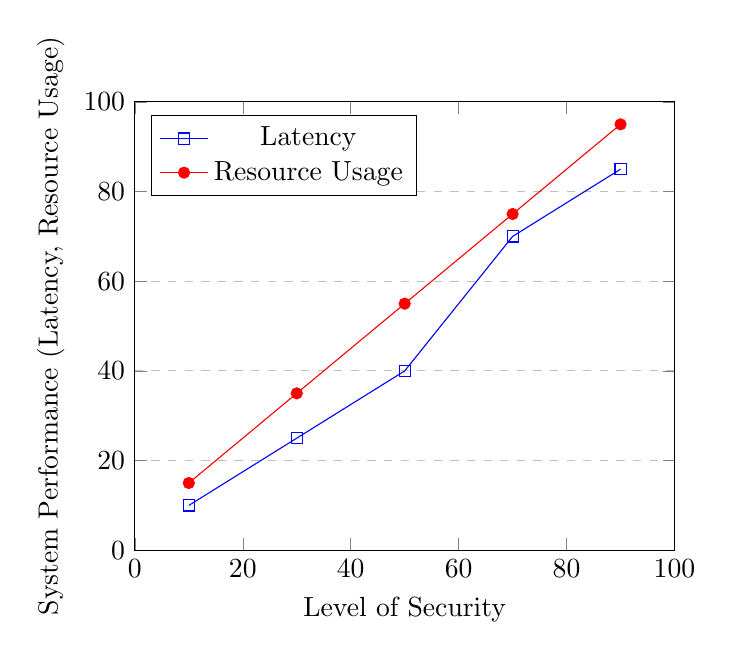
\begin{tikzpicture}
\begin{axis}[
    xlabel={Level of Security},
    ylabel={System Performance (Latency, Resource Usage)},
    xmin=0, xmax=100,
    ymin=0, ymax=100,
    legend pos=north west,
    ymajorgrids=true,
    grid style=dashed,
]
\addplot[
    color=blue,
    mark=square,
    ]
    coordinates {
    (10,10)(30,25)(50,40)(70,70)(90,85)
    };
\addlegendentry{Latency}

\addplot[
    color=red,
    mark=*,
    ]
    coordinates {
    (10,15)(30,35)(50,55)(70,75)(90,95)
    };
\addlegendentry{Resource Usage}

\end{axis}
\end{tikzpicture}
\caption{Impact of Security Measures on CPS Performance}
\label{fig:security_performance}
\end{figure}



\begin{table*}[h]
\centering
\caption{Overview of CPS Security Challenges, Impacts, and Mitigation Strategies}
\label{tab:cps_challenges}
\begin{tabular}{|p{4cm}|p{5cm}|p{5cm}|}
\hline
\textbf{Security Challenge} & \textbf{Impact} & \textbf{Mitigation Strategies} \\ \hline
Resource Constraints & Difficulty in applying strong security measures such as encryption due to limited computational capacity. & Use of lightweight cryptographic algorithms (e.g., ECC) and efficient anomaly detection techniques. \\ \hline
Legacy Systems & High vulnerability due to outdated protocols and hardware, leading to increased security risks. & Network segmentation, virtual patching, and incremental replacement of legacy components. \\ \hline
Cross-Domain Complexity & Integrated physical and cyber components create multiple attack surfaces, leading to increased risk of cyber-physical attacks. & Hybrid security approaches that monitor both physical and digital components simultaneously. \\ \hline
Scalability Issues & Difficulty in managing large numbers of interconnected devices, leading to cascading failure risks. & Hierarchical security management and segmentation to isolate failures and reduce overall risk. \\ \hline
Insider Threats & Harder to detect due to existing system privileges, posing risks of malicious or accidental attacks. & Multi-factor authentication (MFA), role-based access control (RBAC), and user behavior analytics (UBA). \\ \hline
Advanced Threats (e.g., Zero-day) & Vulnerabilities that are exploited before they can be patched, leading to potential system compromises. & Proactive threat modeling, rapid patch management, and machine learning-based detection systems. \\ \hline
\end{tabular}
\end{table*}



\usepackage{pgfplots}

\begin{figure}[h]
\centering
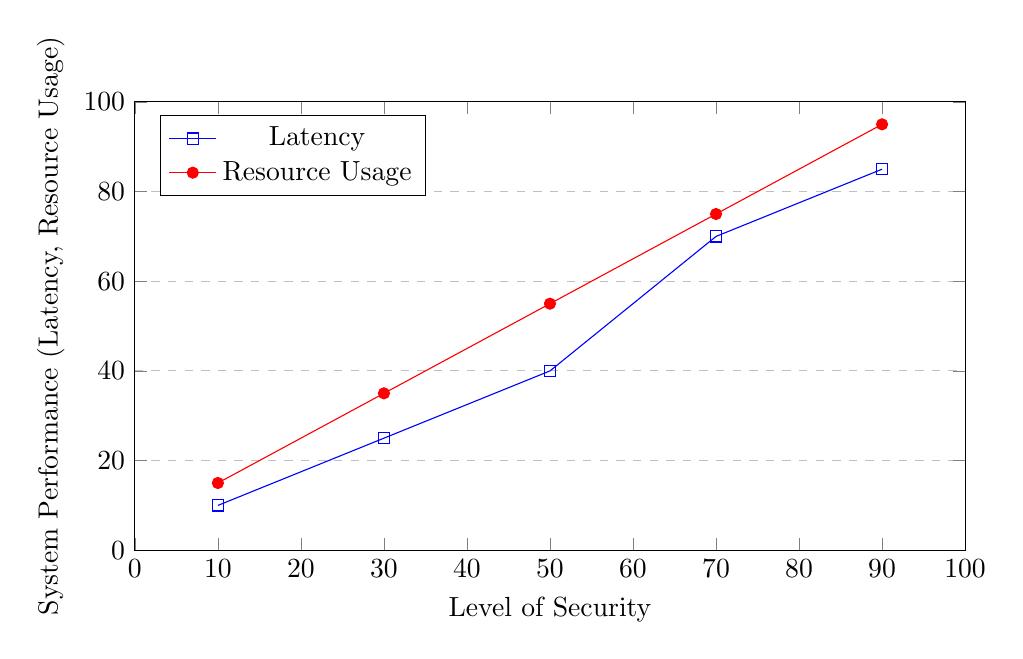
\begin{tikzpicture}
\begin{axis}[
    width=\linewidth,
    height=0.6\linewidth,
    xlabel={Level of Security},
    ylabel={System Performance (Latency, Resource Usage)},
    xmin=0, xmax=100,
    ymin=0, ymax=100,
    legend pos=north west,
    ymajorgrids=true,
    grid style=dashed,
]
% Plot for Latency
\addplot[
    color=blue,
    mark=square,
    ]
    coordinates {
    (10,10)(30,25)(50,40)(70,70)(90,85)
    };
\addlegendentry{Latency}

% Plot for Resource Usage
\addplot[
    color=red,
    mark=*,
    ]
    coordinates {
    (10,15)(30,35)(50,55)(70,75)(90,95)
    };
\addlegendentry{Resource Usage}

\end{axis}
\end{tikzpicture}
\caption{Impact of Security Measures on CPS Performance}
\label{fig:security_performance}
\end{figure}




\usetikzlibrary{shapes.geometric, arrows}

\tikzstyle{startstop} = [rectangle, rounded corners, minimum width=3cm, minimum height=1cm,text centered, draw=black, fill=red!30]
\tikzstyle{process} = [rectangle, minimum width=3cm, minimum height=1cm, text centered, draw=black, fill=orange!30]
\tikzstyle{decision} = [diamond, minimum width=3cm, minimum height=1cm, text centered, draw=black, fill=green!30]
\tikzstyle{arrow} = [thick,->,>=stealth]

\begin{figure*}[h]
\centering
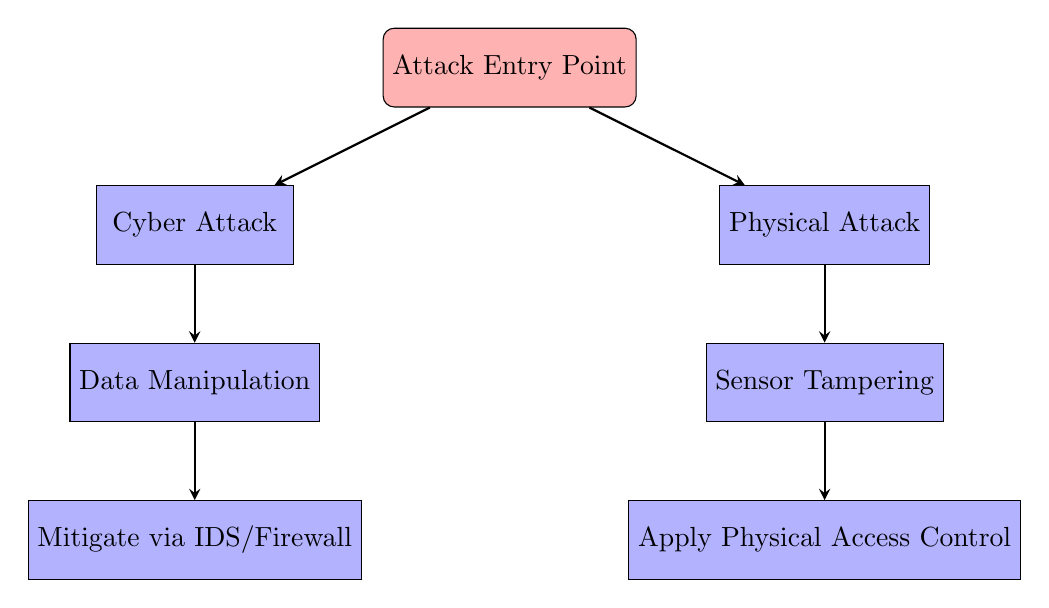
\begin{tikzpicture}[node distance=2cm]

% Nodes
\node (start) [startstop] {Attack Entry Point};
\node (cyber) [process, below of=start, xshift=-4cm] {Cyber Attack};
\node (physical) [process, below of=start, xshift=4cm] {Physical Attack};
\node (databreach) [process, below of=cyber] {Data Manipulation};
\node (tampering) [process, below of=physical] {Sensor Tampering};
\node (response1) [process, below of=databreach] {Mitigate via IDS/Firewall};
\node (response2) [process, below of=tampering] {Apply Physical Access Control};

% Arrows
\draw [arrow] (start) -- (cyber);
\draw [arrow] (start) -- (physical);
\draw [arrow] (cyber) -- (databreach);
\draw [arrow] (physical) -- (tampering);
\draw [arrow] (databreach) -- (response1);
\draw [arrow] (tampering) -- (response2);

\end{tikzpicture}
\caption{Attack Vectors and Response Pathways in CPS}
\label{fig:attack_pathways}
\end{figure*}




\usetikzlibrary{shapes, arrows, positioning}

\begin{figure*}[h]
\centering
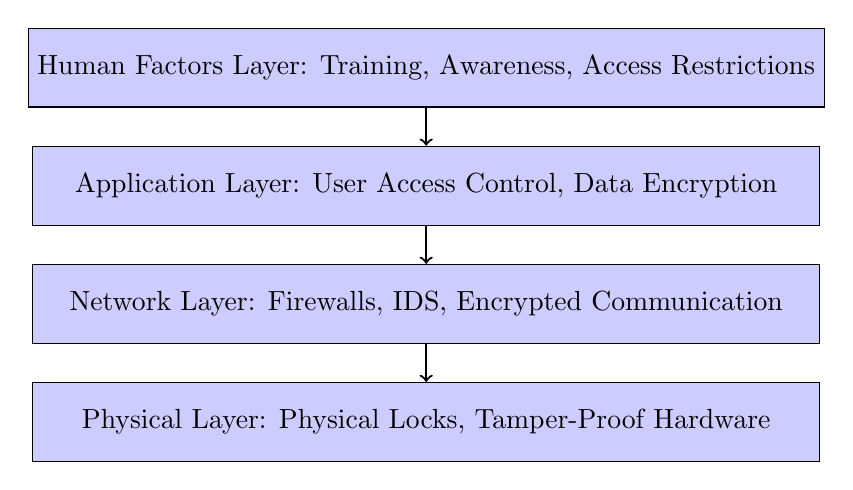
\begin{tikzpicture}[
    layer/.style={rectangle, draw=black, fill=blue!20, text centered, minimum width=10cm, minimum height=1cm},
    yscale=1.5
]

% Layers
\node[layer] (human) at (0,4) {Human Factors Layer: Training, Awareness, Access Restrictions};
\node[layer] (app) at (0,3) {Application Layer: User Access Control, Data Encryption};
\node[layer] (network) at (0,2) {Network Layer: Firewalls, IDS, Encrypted Communication};
\node[layer] (physical) at (0,1) {Physical Layer: Physical Locks, Tamper-Proof Hardware};

% Arrows
\draw[->, thick] (human.south) -- (app.north);
\draw[->, thick] (app.south) -- (network.north);
\draw[->, thick] (network.south) -- (physical.north);

\end{tikzpicture}
\caption{Security Layers in CPS Architecture}
\label{fig:security_layers}
\end{figure*}
\end{comment}

\section{CPS Security Challenges}\label{sec:challenges}
\begin{figure*}
\centering
\includegraphics[width=1\textwidth]{images/Schema.png}
\caption{Overview of CPS Security Challenges and Their Classifications}
\label{fig:overview-cps-challenges}
\end{figure*}


CPS face a wide range of security challenges due to their combination of digital and physical components. These systems, which are used in areas like healthcare, transportation, and critical infrastructure, must handle threats from both cyber and physical domains. The complexity of these systems makes them difficult to protect. To better understand these security issues, we can group them into four themes: system-level vulnerabilities, threats and attack types, security measures and responses, and external factors such as regulations, privacy concerns, and the human element \cite{166,167,168,169,170,171,172,173,174,175,176,177,178,179,180,181,182,183,184,185,186,187}. This section provides an integrated analysis of these challenges and explores possible solutions.

\subsection{System-Level Vulnerabilities and Constraints}

CPS face significant system-level vulnerabilities that stem from the resource limitations of their components, the cross-domain complexity of their architecture, and the continued use of legacy systems. Devices in CPS environments, such as sensors and actuators, often have constrained computational power, memory, and energy resources, making it difficult to implement standard security mechanisms like encryption and intrusion detection \cite{30,34,36}. These constraints are further compounded by the need for CPS to operate continuously without downtime, particularly in sectors where real-time operation is critical, such as healthcare and ICS\cite{31,36}. As a result, these systems cannot afford delays due to complex security updates or processes. To tackle these limitations, lightweight security solutions such as elliptic curve cryptography (ECC) and efficient anomaly detection techniques are increasingly adopted to balance the need for security with performance demands \cite{30,34}.

The cross-domain nature of CPS adds another layer of complexity to their security. Unlike traditional IT systems, CPS integrate both physical components such as machines, robots, and sensors with cyber elements, including networks and software \cite{209}. This tight coupling of the physical and cyber domains creates vulnerabilities that can be exploited by attackers in multiple ways \cite{31,34}. Attacks on CPS can target either the digital or the physical components; for instance, cyberattacks can manipulate sensor readings, while physical attacks can directly affect actuators or other hardware. Such attacks can lead to not only data breaches but also physical damage or significant threats to human safety \cite{30,34,40}.

Legacy systems pose additional challenges. Many CPS environments, particularly in critical infrastructure like power generation and healthcare, rely on legacy hardware and outdated protocols that were not designed with modern cybersecurity threats in mind \cite{40,42}. Updating or replacing these systems is often cost-prohibitive and operationally risky, leading to continued reliance on technology that lacks essential security capabilities. To mitigate the risks associated with these legacy systems, practices such as network segmentation and virtual patching are often used to create temporary security barriers \cite{40,42}.

The interconnectedness and scale of CPS also lead to challenges related to scalability and cascading effects. In large scale CPS networks such as smart cities or extensive industrial operations thousands of devices are interconnected, increasing the attack surface. If a single vulnerable component is compromised, it can trigger cascading failures that affect the entire system \cite{36,38}. For instance, a compromised sensor in a power grid could lead to widespread blackouts, as was observed in the 2003 Northeast blackout, where a failure in a single monitoring tool had far-reaching consequences \cite{37,41}. Hierarchical security management, where local control points are established to manage smaller segments of the network, is one approach that can help mitigate these risks by isolating failures and reducing overall system vulnerability \cite{37,41}.

\subsection{Threats and Attack Vectors}

CPS are exposed to a broad spectrum of threats, from traditional cyberattacks to physical sabotage, due to the diverse ways in which these systems operate and interact. One of the critical security challenges lies in the range and diversity of potential attack vectors. Digital attacks, such as malware, denial of service (DoS) attacks, and advanced persistent threats (APTs), can manipulate data or disrupt system operations \cite{30,34,40,201}. Meanwhile, physical threats such as tampering with sensors or other hardware can compromise the integrity of the physical components of the system \cite{30,34}. This dual nature of threats makes CPS security inherently more complex compared to traditional IT systems.

\begin{comment}
\begin{figure}[h]
\centering
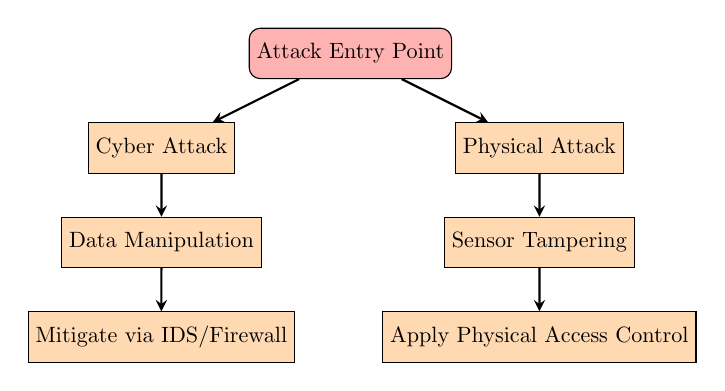
\begin{tikzpicture}[node distance=1.5cm, scale=0.8, every node/.style={transform shape}]
\tikzstyle{startstop} = [rectangle, rounded corners, minimum width=2.2cm, minimum height=0.8cm, text centered, draw=black, fill=red!30]
\tikzstyle{process} = [rectangle, minimum width=2.2cm, minimum height=0.8cm, text centered, draw=black, fill=orange!30]
\tikzstyle{arrow} = [thick,->,>=stealth]

% Nodes
\node (start) [startstop] {Attack Entry Point};
\node (cyber) [process, below of=start, xshift=-3cm] {Cyber Attack};
\node (physical) [process, below of=start, xshift=3cm] {Physical Attack};
\node (databreach) [process, below of=cyber] {Data Manipulation};
\node (tampering) [process, below of=physical] {Sensor Tampering};
\node (response1) [process, below of=databreach] {Mitigate via IDS/Firewall};
\node (response2) [process, below of=tampering] {Apply Physical Access Control};

% Arrows
\draw [arrow] (start) -- (cyber);
\draw [arrow] (start) -- (physical);
\draw [arrow] (cyber) -- (databreach);
\draw [arrow] (physical) -- (tampering);
\draw [arrow] (databreach) -- (response1);
\draw [arrow] (tampering) -- (response2);

\end{tikzpicture}
\caption{Attack Vectors and Response Pathways in CPS}
\label{fig:attack_pathways}
\end{figure}
\end{comment}


\begin{figure}[h]
\centering
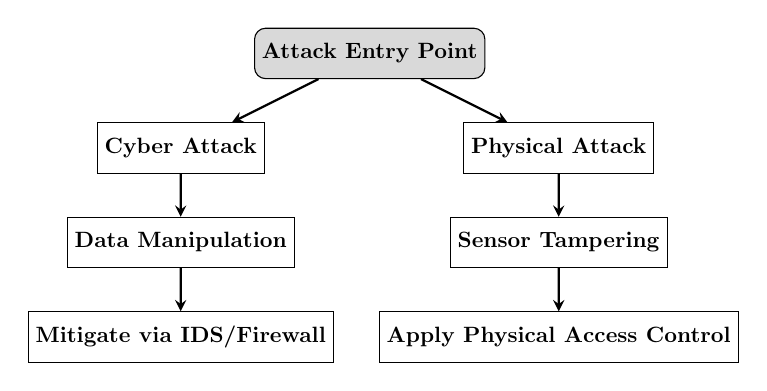
\begin{tikzpicture}[node distance=1.5cm, scale=0.8, every node/.style={transform shape}]
\tikzstyle{startstop} = [rectangle, rounded corners, minimum width=2.2cm, minimum height=0.8cm, text centered, draw=black, fill=gray!30]
\tikzstyle{process} = [rectangle, minimum width=2.2cm, minimum height=0.8cm, text centered, draw=black, fill=white]
\tikzstyle{arrow} = [thick,->,>=stealth, draw=black]

% Nodes
\node (start) [startstop] {\textbf{Attack Entry Point}};
\node (cyber) [process, below of=start, xshift=-3cm] {\textbf{Cyber Attack}};
\node (physical) [process, below of=start, xshift=3cm] {\textbf{Physical Attack}};
\node (databreach) [process, below of=cyber] {\textbf{Data Manipulation}};
\node (tampering) [process, below of=physical] {\textbf{Sensor Tampering}};
\node (response1) [process, below of=databreach] {\textbf{Mitigate via IDS/Firewall}};
\node (response2) [process, below of=tampering] {\textbf{Apply Physical Access Control}};

% Arrows
\draw [arrow] (start) -- (cyber);
\draw [arrow] (start) -- (physical);
\draw [arrow] (cyber) -- (databreach);
\draw [arrow] (physical) -- (tampering);
\draw [arrow] (databreach) -- (response1);
\draw [arrow] (tampering) -- (response2);

\end{tikzpicture}
\caption{The figure depicts typical attack entry points and the corresponding mitigation strategies in CPS, showcasing both digital and physical threat vectors.}
\label{fig:attack_pathways}
\end{figure}





Advanced threats, such as zero-day vulnerabilities, present a particularly serious risk to CPS because these vulnerabilities are often unknown to developers and security professionals \cite{203}, allowing attackers to exploit them before they are patched \cite{34,36,37}. Moreover, attackers are increasingly leveraging AI to identify vulnerabilities or automate coordinated attacks, further complicating defense mechanisms. Such attacks are difficult to detect because they may bypass conventional security measures, leading to potentially catastrophic outcomes, especially in critical systems like autonomous vehicles or industrial automation \cite{34,36}.

Insider threats add an additional dimension to the risk landscape of CPS. Insiders, such as employees or contractors, already have legitimate access to the system, making their actions difficult to detect and mitigate \cite{35,39}. These threats may be malicious or unintentional; for instance, a well-meaning employee could inadvertently misconfigure a device, introducing vulnerabilities. Mitigating these threats requires implementing robust access controls, such as multi-factor authentication (MFA) and role-based access control (RBAC), and using user behavior analytics (UBA) to detect abnormal activities that might indicate an insider threat \cite{35,39}.

Figure \ref{fig:attack_pathways} illustrates the typical attack entry points in CPS, categorizing them into cyber attacks and physical attacks, along with corresponding mitigation strategies that address digital threats through IDS/Firewalls and physical threats via access control measures.
\subsection{Security Measures and Responses}

Effective CPS security demands a comprehensive approach that integrates multiple protective measures across both the cyber and physical domains. Traditional security tools, such as firewalls and network-based intrusion detection systems, are insufficient on their own, as CPS require defenses that span both digital data flows and physical operations \cite{30,33}. An emerging approach to enhance CPS security involves using hybrid intrusion detection systems that combine machine learning-based anomaly detection with traditional signature-based techniques. These hybrid systems are particularly effective at identifying both known and emerging threats, providing a more holistic defense against complex attack scenarios \cite{30,33}.

Another essential aspect of securing CPS is ensuring resilience in the face of attacks. CPS must be capable of detecting and isolating security breaches swiftly while continuing to operate without causing harm \cite{33,41}. For example, in a smart grid, if one segment is compromised, other parts of the grid must maintain functionality to prevent a large-scale blackout. Resilience can be built into CPS through redundancy, failover mechanisms, and segmentation, allowing the system to withstand localized attacks without experiencing total failure \cite{33,41}.

\begin{figure}[h]
\centering
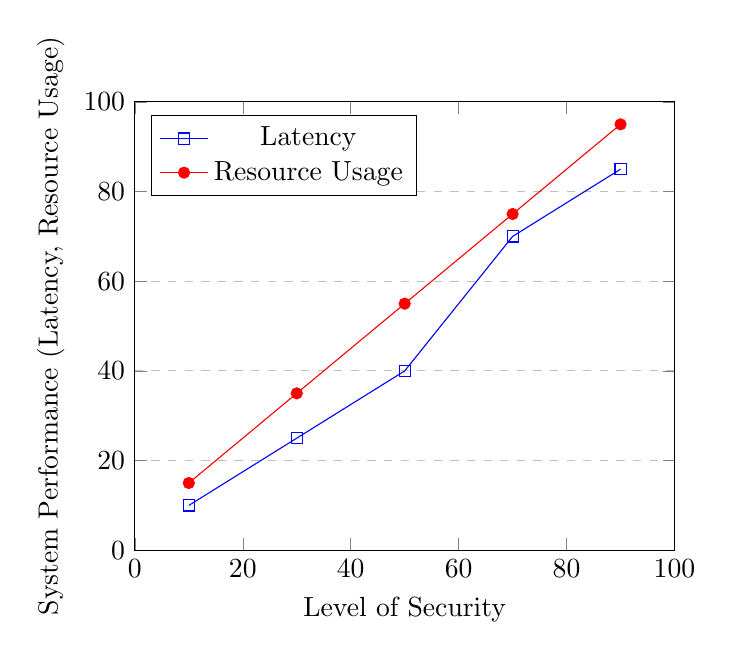
\begin{tikzpicture}
\begin{axis}[
    xlabel={Level of Security},
    ylabel={System Performance (Latency, Resource Usage)},
    xmin=0, xmax=100,
    ymin=0, ymax=100,
    legend pos=north west,
    ymajorgrids=true,
    grid style=dashed,
]
\addplot[
    color=blue,
    mark=square,
    ]
    coordinates {
    (10,10)(30,25)(50,40)(70,70)(90,85)
    };
\addlegendentry{Latency}

\addplot[
    color=red,
    mark=*,
    ]
    coordinates {
    (10,15)(30,35)(50,55)(70,75)(90,95)
    };
\addlegendentry{Resource Usage}

\end{axis}
\end{tikzpicture}
\caption{Impact of Security Measures on CPS Performance}
\label{fig:security_performance}
\end{figure}

The need for real-time responsiveness is another critical factor in CPS security. Implementing advanced security measures, such as encryption or multifactor authentication, can sometimes introduce latency, which can be unacceptable in systems requiring immediate response, such as healthcare devices or autonomous vehicles \cite{30,31,33}. Figure~\ref{fig:security_performance} illustrates how increasing levels of security impact key performance metrics like latency and resource usage, highlighting the importance of balancing security with operational efficiency. Recent advances, like homomorphic encryption enabling operations on encrypted data without decryption and edge computing processing data closer to the source can offer solutions that enhance security while maintaining the necessary performance levels \cite{30,31,33}.

\subsection{Regulatory, Privacy, and Human Factors}

Beyond the technical challenges, CPS security is also influenced by regulatory, privacy, and human factors. The regulatory landscape for CPS is fragmented, with some sectors, such as electric power, adopting rigorous standards like the North American Electric Reliability Corporation (NERC) guidelines, while others lack comprehensive regulations \cite{30,32,42}. This inconsistency creates gaps in the security posture of different CPS sectors. Developing a unified international regulatory framework drawing on models like ISO/IEC 27001 but tailored for CPS environments could help establish a standardized level of security across industries.
\begin{comment}
    
\begin{figure}[h]
\centering
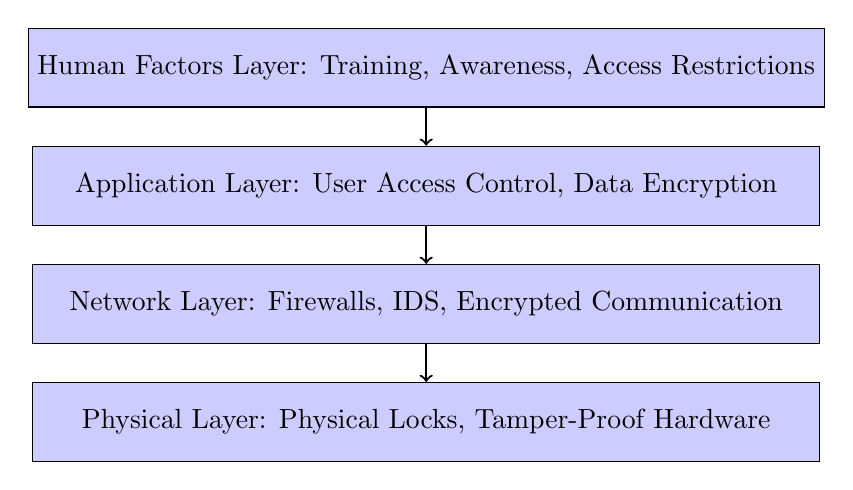
\begin{tikzpicture}[
    layer/.style={rectangle, draw=black, fill=blue!20, text centered, minimum width=10cm, minimum height=1cm},
    yscale=1.5
]

% Layers
\node[layer] (human) at (0,4) {Human Factors Layer: Training, Awareness, Access Restrictions};
\node[layer] (app) at (0,3) {Application Layer: User Access Control, Data Encryption};
\node[layer] (network) at (0,2) {Network Layer: Firewalls, IDS, Encrypted Communication};
\node[layer] (physical) at (0,1) {Physical Layer: Physical Locks, Tamper-Proof Hardware};

% Arrows
\draw[->, thick] (human.south) -- (app.north);
\draw[->, thick] (app.south) -- (network.north);
\draw[->, thick] (network.south) -- (physical.north);

\end{tikzpicture}
\caption{Security Layers in CPS Architecture}
\label{fig:security_layers}
\end{figure}
\end{comment}

\begin{comment}
\begin{table}[h]
\centering
\caption{Some Impact and Mitigation Strategies of CPS Security Challenges}
\label{tab:cps_challenges}
\begin{tabular}{|p{1.5cm}|p{3cm}|p{3cm}|}
\hline
\textbf{Security Challenge} & \textbf{Impact} & \textbf{Mitigation Strategies} \\ \midrule
Resource Constraints & Difficulty in applying strong security measures such as encryption due to limited computational capacity. & Use of lightweight cryptographic algorithms (e.g., ECC) and efficient anomaly detection techniques \cite{30,34,36}. \\ \midrule
Legacy Systems & High vulnerability due to outdated protocols and hardware, leading to increased security risks. & Network segmentation, virtual patching, and incremental replacement of legacy components \cite{40,42}. \\ \midrule
Cross-Domain Complexity & Integrated physical and cyber components create multiple attack surfaces, leading to increased risk of cyber-physical attacks. & Hybrid security approaches that monitor both physical and digital components simultaneously \cite{31,34}. \\ \midrule
Scalability Issues & Difficulty in managing large numbers of interconnected devices, leading to cascading failure risks. & Hierarchical security management and segmentation to isolate failures and reduce overall risk \cite{36,38}. \\ \midrule
Insider Threats & Harder to detect due to existing system privileges, posing risks of malicious or accidental attacks. & Multi-factor authentication (MFA), role-based access control (RBAC), and user behavior analytics (UBA) \cite{35,39}. \\ \midrule
Advanced Threats (e.g., Zero-day) & Vulnerabilities that are exploited before they can be patched, leading to potential system compromises. & Proactive threat modeling, rapid patch management, and machine learning-based detection systems \cite{34,36,37}. \\ \midrule
\end{tabular}
\end{table}
\end{comment}



\begin{table*}[h]
\centering
\caption{Some Impact and Mitigation Strategies of CPS Security Challenges}
\label{tab:cps_challenges}
\renewcommand{\arraystretch}{1.3}
\begin{tabularx}{\textwidth}{@{}p{2.5cm}X X@{}}
\toprule
\textbf{Security Challenge} & \textbf{Impact} & \textbf{Mitigation Strategies} \\
\midrule
Resource Constraints & Difficulty in applying strong security measures such as encryption due to limited computational capacity. & Use of lightweight cryptographic algorithms (e.g., ECC) and efficient anomaly detection techniques \cite{30,34,36} \\
\addlinespace
\rowcolor[HTML]{EFEFEF}
Legacy Systems & High vulnerability due to outdated protocols and hardware, leading to increased security risks. & Network segmentation, virtual patching, and incremental replacement of legacy components \cite{40,42} \\
\addlinespace

Cross-Domain Complexity & Integrated physical and cyber components create multiple attack surfaces, leading to increased risk of cyber-physical attacks. & Hybrid security approaches that monitor both physical and digital components simultaneously \cite{31,34} \\
\addlinespace
\rowcolor[HTML]{EFEFEF}
Scalability Issues & Difficulty in managing large numbers of interconnected devices, leading to cascading failure risks. & Hierarchical security management and segmentation to isolate failures and reduce overall risk \cite{36,38} \\
\addlinespace
Insider Threats & Harder to detect due to existing system privileges, posing risks of malicious or accidental attacks. & Multi-factor authentication (MFA), role-based access control (RBAC), and user behavior analytics (UBA) \cite{35,39} \\
\addlinespace
\rowcolor[HTML]{EFEFEF}
Advanced Threats& Vulnerabilities that are exploited before they can be patched, leading to potential system compromises. & Proactive threat modeling, rapid patch management, and machine learning-based detection systems \cite{34,36,37} \\
\bottomrule
\end{tabularx}
\end{table*}

\begin{comment}
\begin{table*}[htbp]
\centering
\caption{Some Impact and Mitigation Strategies of CPS Security Challenges}
\label{tab:cps_challenges}
\renewcommand{\arraystretch}{1.3}  % Increase vertical spacing
\begin{tabular}{|p{2.5cm}|p{5cm}|p{5cm}|}
\hline
\rowcolor{gray!10}  % Add light gray background to header
\textbf{Security Challenge} & \textbf{Impact} & \textbf{Mitigation Strategies} \\
\hline
\textbf{Resource Constraints} & 
Difficulty in applying strong security measures such as encryption due to limited computational capacity. & 
Use of lightweight cryptographic algorithms (e.g., ECC) and efficient anomaly detection techniques \cite{30,34,36}. \\
\hline
\rowcolor{gray!5}  % Alternate row color
\textbf{Legacy Systems} & 
High vulnerability due to outdated protocols and hardware, leading to increased security risks. & 
Network segmentation, virtual patching, and incremental replacement of legacy components \cite{40,42}. \\
\hline
\textbf{Cross-Domain Complexity} & 
Integrated physical and cyber components create multiple attack surfaces, leading to increased risk of cyber-physical attacks. & 
Hybrid security approaches that monitor both physical and digital components simultaneously \cite{31,34}. \\
\hline
\rowcolor{gray!5}  % Alternate row color
\textbf{Scalability Issues} & 
Difficulty in managing large numbers of interconnected devices, leading to cascading failure risks. & 
Hierarchical security management and segmentation to isolate failures and reduce overall risk \cite{36,38}. \\
\hline
\textbf{Insider Threats} & 
Harder to detect due to existing system privileges, posing risks of malicious or accidental attacks. & 
Multi-factor authentication (MFA), role-based access control (RBAC), and user behavior analytics (UBA) \cite{35,39}. \\
\hline
\rowcolor{gray!5}  % Alternate row color
\textbf{Advanced Threats} \newline (e.g., Zero-day) & 
Vulnerabilities that are exploited before they can be patched, leading to potential system compromises. & 
Proactive threat modeling, rapid patch management, and machine learning-based detection systems \cite{34,36,37}. \\
\hline
\end{tabular}
\end{table*}

    
\end{comment}


Data integrity and privacy are also critical concerns. CPS often collect significant amounts of sensitive data, especially in applications like healthcare and smart cities \cite{31,36,38}. Ensuring this data remains secure from unauthorized access is crucial to preventing attackers from manipulating system behavior. At the same time, privacy must be maintained, particularly where personal user data is involved. Designers need to strike a delicate balance between functionality and privacy by integrating privacy-by-design principles into CPS development \cite{31,36}.

Human factors, particularly the lack of specialized security training among CPS operators and engineers, pose additional challenges. Many employees responsible for managing CPS do not have sufficient training to recognize or mitigate security threats effectively \cite{39,43}. Programs like the NIST Cybersecurity Workforce Framework can provide organizations with a structure to identify skill gaps and improve security awareness through training and education. Enhancing workforce competence is crucial for preventing unintentional security breaches and ensuring that CPS are properly managed and protected \cite{39,43}.

Table \ref{tab:cps_challenges} provides some examples of CPS security challenges, illustrating their impacts and mitigation strategies, such as the use of lightweight cryptographic algorithms for addressing resource constraints and hybrid security approaches for managing cross-domain complexity.

The security of CPS is shaped by a multitude of interrelated challenges that include technical limitations, complex attack vectors, the need for specialized security measures, and broader regulatory and human factors. Addressing these challenges requires an integrated approach that combines technological innovation, strategic policy-making, and investment in human capital \cite{188,189,190,191,192,193}. Such a comprehensive strategy will be essential to secure CPS as they continue to expand and play an increasingly critical role in our interconnected world. Diagram \ref{fig:overview-cps-challenges} provides a structured overview of the primary security challenges in CPS, categorized into system vulnerabilities, attack vectors, mitigation measures, and external factors.

%\section{Invariant Rules}

\begin{definition}
Invariant rules are defined as physical conditions that must be satisfied for any given state of an Industrial Control System (ICS). These rules are derived from the operational data of the ICS and describe the expected relationships between sensor readings and actuator states. If these conditions are violated, it indicates a deviation from normal operation, which can be used to detect anomalies in the system. The rules help identify whether the system is operating within its normal parameters or if any unusual activities could signify faults or cyber-attacks\cite{21}. Invariants are stable relationships or dependencies between different components of a system that remain consistent under normal operating conditions. Detecting these invariants is crucial for monitoring system health and identifying anomalies when these relationships break\cite{23}.
\end{definition}
The proposed framework introduces a novel, systematic approach to automatically generating invariant rules from data logs of Industrial Control Systems (ICS) to enhance anomaly detection. Invariant rules, which define the normal operational conditions of ICS by specifying physical relationships between sensors and actuators, are essential for identifying deviations that could signify faults or cyber-attacks. Traditionally, these rules are manually defined by system engineers based on design specifications, a process that is both costly and prone to errors, especially in complex systems. To overcome these limitations, our framework leverages machine learning and data mining techniques to automatically derive invariant rules directly from historical operational data logs.

The process begins with data collection, where sensor measurements and actuator states are recorded over time during the normal operation of the ICS. This data is then processed to generate "predicates," or conditions that describe specific states or relationships within the system. Predicates for actuator states are straightforward, while predicates for continuous sensor readings are generated using two strategies: a distribution-driven strategy that models sensor reading updates using Gaussian Mixture Models (GMMs) to identify hidden control states, and an event-driven strategy that identifies critical sensor values that trigger changes in actuator states.

Once the predicates are generated, the framework converts each data log entry into an "itemset"—a collection of satisfied predicates—and applies association rule mining to discover meaningful invariant rules. These rules are defined as those that meet a minimum support condition, ensuring they are statistically significant, and are non-redundant, providing unique information that is not captured by other rules. To optimize the number of generated rules while minimizing false positives, the framework incorporates a parameter tuning process using a validation dataset. This process fine-tunes the parameters to balance rule generation with the expected false positive rate, ensuring the model is both effective and efficient for real-time anomaly detection.

The generated rules are then applied to real-time operational data to detect anomalies, with each data entry checked against the rules. Violations indicate potential anomalies, prompting further investigation or immediate response. This data-driven approach is validated through case studies on two real-world ICS testbeds, demonstrating significantly improved anomaly detection performance over traditional design-based and residual error-based models. The framework not only automates the rule generation process but also provides a robust, scalable solution for enhancing ICS security, capable of adapting to the evolving nature of industrial environments and threats.\cite{21}(invariant and detection)

$$**************************$$

ARTINALI is a dynamic invariant detection approach specifically designed to enhance the security of Cyber-Physical Systems (CPS) by incorporating time as a fundamental property alongside data and events. The process begins with the instrumentation of the CPS source code to monitor and log key events, data variables, and time information. Events, such as system calls or significant operations like reading a sensor value or sending a network packet, are identified and logged during normal (attack-free) operation. The collected logs provide detailed execution traces, including event types, data states, and timestamps, which are essential for the subsequent invariant mining process.

ARTINALI mines three types of invariants from these execution traces: Data per Event (D|E), Event per Time (E|T), and Data per Time (D|T). The D|E invariants capture the relationships between data variables and specific events by grouping the system logs by event and applying frequent item set mining to identify common data patterns associated with each event. For instance, if a variable like \texttt{temperature} always falls within a certain range during a specific event like ``sensor\_read,'' a D|E invariant would specify this range for that event. E|T invariants are then derived to understand the timing relationships between events. This involves identifying sequences of events and calculating the typical time intervals between them. For example, an E|T invariant might state that the event ``send\_data'' should always follow ``sensor\_read'' within a specific time window, such as 5 to 10 seconds. Finally, ARTINALI combines the D|E and E|T invariants to infer D|T invariants, which describe how data values change over time in relation to events. This process involves calculating the conditional probabilities of data values occurring within specific time intervals between events, providing a comprehensive understanding of the temporal data relationships.

The mined invariants are then used to configure an Intrusion Detection System (IDS) that continuously monitors the CPS for deviations from these learned invariants. During runtime, if an event occurs outside its typical time window, if a data variable takes on an unexpected value, or if there is any deviation from the established patterns, the IDS flags a potential intrusion or anomaly. For example, in a smart meter system, if the event ``send\_data'' occurs much later than the expected time following ``process\_data,'' or if the power consumption data suddenly falls outside its normal range, the IDS would detect these deviations as potential security threats. By dynamically detecting invariants that consider the interplay between data, events, and time, ARTINALI significantly reduces false positives and negatives, providing a robust framework for real-time CPS security\cite{22}.

\textbf{Different. }The ARTINALI paper differentiates itself from other research in the field of Cyber-Physical System (CPS) security by introducing a novel approach that incorporates time as a first-class property alongside data and events for dynamic invariant detection. Unlike traditional methods that focus solely on data or event relationships, ARTINALI mines multi-dimensional invariants by considering data, events, and time simultaneously, providing a more comprehensive model of system behavior. This integration significantly reduces false positives and negatives, enhancing the accuracy of intrusion detection systems (IDS) for CPS. The paper demonstrates ARTINALI's effectiveness on real-world CPS platforms, such as smart meters and smart medical devices, showing substantial improvements over existing tools. By effectively capturing the complex interactions within CPS and improving real-time monitoring capabilities, ARTINALI offers a robust framework for detecting sophisticated attacks, laying a foundation for future advancements in CPS security.

$$************************$$

illiad detects invariants in cyber-physical systems (CPS) through a systematic approach that combines data-driven and model-based methodologies to monitor the system's normal operating conditions and identify anomalies. The first step in the process involves collecting and preparing data from various sensors and devices within the CPS. In a typical example, such as a microgrid with a solar panel, battery storage system, and local load, sensors would gather time-series data on variables like solar power output, battery state of charge (SOC), and load power consumption. This data is then preprocessed to address missing values and noise, ensuring it is normalized and consistent for further analysis.

The next step is to define the invariants and dependencies within the system. Invariants are stable relationships between components that remain consistent under normal operating conditions. For instance, in the microgrid example, an invariant might be the relationship between battery SOC, solar power output, and load power. If solar power output is high and load power is low, it is expected that the battery charges, leading to an increase in SOC. illiad aims to detect these kinds of relationships to monitor the system's health.

To detect these invariants, illiad utilizes a hybrid approach combining three primary techniques: Autoregressive Models with Exogenous Inputs (ARX), Latent Factor Analysis (LFA), and Kalman Filter-Based State Estimation. ARX models predict a time series, such as battery SOC, based on its own past values and the past values of other related series, like solar power and load power. If the prediction error of an ARX model remains consistently low, illiad infers a stable invariant relationship between the components. Latent Factor Analysis is then employed to uncover hidden relationships that may not be directly observable but are inferred through latent variables influencing multiple observed variables. For example, a latent factor might represent an underlying environmental condition, such as sunlight availability, affecting both solar power output and load power. Finally, Kalman Filters are used for dynamic state estimation, combining current measurements with previous state estimates to predict the system's state. If Kalman filters accurately estimate the state over time, a strong invariant relationship is inferred.

Once these models have been applied, illiad integrates the results to construct an invariant graph, where each node represents a system component and each edge represents an inferred invariant relationship. The system selects the strongest relationships—those with the least prediction error—from the ARX, LFA, and Kalman Filter models. Thresholds are applied to ensure that only meaningful, stable relationships are included as invariants in the graph. For example, if ARX predicts battery SOC with less than a 5\% error but LFA has a 10\% error, ARX would be selected as the basis for the invariant. The final invariant graph provides a comprehensive view of the system's normal operating conditions.

illiad continuously monitors these invariant relationships in real-time to detect any deviations that might indicate anomalies. An anomaly is detected when a relationship deviates beyond acceptable limits, indicating a possible fault or failure in the system. For example, if the battery SOC decreases unexpectedly despite high solar power and low load power, this could signal a malfunctioning battery. When an anomaly is detected, illiad issues an alert, highlighting the broken invariant and pinpointing the component potentially causing the issue.

To facilitate real-time monitoring and quick response, illiad includes a visual dashboard that displays the invariant graph and highlights any broken invariants as they occur. This interactive dashboard allows operators to drill down into specific components, view historical data, and make informed decisions for troubleshooting and maintenance. By integrating data-driven and model-based approaches, illiad provides a robust framework for detecting invariants, monitoring system health, and promptly identifying anomalies in complex cyber-physical systems\cite{23}.

$$**********************$$

To detect invariants in Cyber-Physical Systems (CPS), they propose a method that combines machine learning with mutation testing. The objective is to learn invariants that define correct CPS behavior and identify deviations indicating faults or malicious activity.

The process begins with collecting two types of sensor data traces: \textit{positive traces}, representing normal behavior, and \textit{negative traces}, representing abnormal behavior. While positive traces are obtained from normal operations, generating negative traces requires simulating faults or security breaches. This is achieved through \textit{mutation testing}, where small changes (mutations) are introduced to the CPS software, simulating faults. Running the mutated software on the CPS or a simulator generates sensor data that serves as negative samples.

Next, they use these traces to train a machine learning model, specifically a Support Vector Machine (SVM), to classify system behavior. The SVM learns to distinguish between normal and abnormal states based on features extracted from the sensor data, such as sensor readings over time. The output is a set of \textit{learned invariants}—conditions that must hold for the system to be considered in a normal state. For example, an invariant might require that a water tank's level remains between specific thresholds.

To ensure these invariants are accurate and reliable, they apply \textit{verification techniques} like statistical model checking and symbolic execution. Statistical model checking provides probabilistic guarantees by analyzing system executions, while symbolic execution verifies invariants against all possible code paths. Together, these techniques validate the learned invariants, ensuring they effectively monitor and control the CPS for safe operation.

This integrated approach leverages the strengths of machine learning, software testing, and formal methods to robustly detect and verify invariants, enhancing the safety and security of CPS in critical applications\cite{24}.

$$*******************************$$

The invariants in the study were detected using \textit{association rule mining}, a data-driven approach that automates the discovery of relationships between system components. The method was applied to data collected from the Secure Water Treatment (SWaT) testbed, a scaled-down version of a water treatment plant designed for cybersecurity research. The dataset contained 11 days of sensor and actuator data, with the first seven days representing normal operations and the remaining days including a series of cyber and physical attacks. This extensive dataset, comprising over 3 million rows, provided the basis for mining relationships between system components.

Before applying the mining algorithm, the data needed to be preprocessed. Sensor and actuator values were numerical and often contained values with several decimal places, making it difficult to generate rules directly. To address this, the researchers categorized the data into discrete ranges, such as "High," "Low," "On," and "Off," based on the operational thresholds of the system. This process transformed the continuous data into categorical data, which is more suitable for association rule mining. By converting the data in this way, the study ensured that the rules generated would be interpretable and aligned with the operational states of the water treatment system.

The researchers then applied the \textit{Apriori algorithm}, a widely used technique in association rule mining, to the preprocessed dataset. The algorithm identifies frequent itemsets—combinations of sensor and actuator states that appear together frequently—and from these itemsets, it generates rules that describe the relationships between different system components. Each rule is evaluated based on its \textit{support}, which measures how often the combination occurs in the dataset, and its \textit{confidence}, which indicates the likelihood that the rule holds true. In total, the algorithm generated approximately 11,500 rules, providing a comprehensive set of constraints that describe the normal behavior of the system.

Once the rules were generated, they were validated by comparing them to known physical invariants derived from the system's design. These known invariants, which were manually defined, served as a benchmark to assess the accuracy of the automatically generated rules. For example, one known invariant is that when a motorized valve (MV101) is open, the flow indicator (FIT101) should display a high value. The Apriori algorithm successfully detected this relationship, with a confidence value of 100\%, indicating that the rule was always observed to be true in the dataset. In contrast, the reverse condition—that FIT101 should not be high when MV101 is closed—had a confidence value of only 0.49\%, further confirming the validity of the automatically generated rules.

While the method successfully detected pairwise relationships between sensors and actuators, it is currently limited in its ability to capture more complex, multi-component interactions that are common in Cyber-Physical Systems (CPS). For example, the behavior of one process may depend on the state of multiple sensors and actuators across different stages of the system. Additionally, the current approach does not account for time-based dependencies, meaning it does not consider how system states evolve over time. Addressing these limitations will be important for future work to improve the accuracy and applicability of the method for detecting cyber-attacks in CPS environments\cite{25}.

$$**************************************$$

The detection of invariants in the proposed approach is carried out using a systematic method called \textit{Design to Invariants (D2I)}. This method derives invariants directly from the design and behavior of the physical process in an Industrial Control System (ICS). The process starts by modeling the ICS using \textit{hybrid automata}, which are formal models capable of representing both the discrete and continuous dynamics of system components. For example, in a water treatment plant, components like pumps and valves are modeled as having discrete states (such as open or closed), while components like tanks are modeled with continuous states (such as varying water levels). The hybrid automaton provides the foundation for understanding how these components behave individually and in combination.

The next step extends the hybrid automata model to better represent the interactions between discrete and continuous states through the use of \textit{state markers} and \textit{invariant multi-graphs}. The state markers define key points in the behavior of continuous components—such as high and low water levels in a tank—that help track the system's evolution. By establishing relationships between these states and the operations of discrete components (such as valves and pumps), \textit{invariants} are derived. These invariants are boolean conditions that must always hold true for the system to be considered operating normally. For instance, an invariant might specify that if a valve is open, the flow rate through a pipe should fall within a particular range. These conditions can be \textit{state-specific}, applying only when the system is in a particular configuration, or \textit{state-agnostic}, applying universally throughout the system's operation.

Once derived, the invariants are \textit{coded and installed in the Programmable Logic Controllers (PLCs)} that manage the physical processes within the ICS. These PLCs continuously monitor the system's state by checking sensor data and actuator operations against the established invariants. When an invariant is violated—meaning the boolean condition returns false—it serves as an indicator of anomalous behavior, which may be due to a cyber attack or a component failure. The invariants act as real-time checks on the system's physical state, ensuring that the ICS behaves as expected according to the system's design.

For example, in a water treatment plant, an invariant might state that when a valve is open and a pump is running, the water level in a connected tank should decrease. If the water level remains constant despite the pump operating, the invariant would be violated, signaling a potential issue. This could indicate a cyber attack, such as a compromised valve that is being falsely reported as open, or a mechanical failure.

The invariants also play a critical role in \textit{detecting cyber attacks}. They capture the expected physical relationships between system components, so if an attacker compromises one or more components, such as by preventing a valve from opening while simultaneously sending false sensor data to the PLC, the violation of an invariant would trigger an alert. Even sophisticated attacks, like \textit{multi-point attacks} that manipulate multiple system elements, can be detected when the combined behavior of the components does not conform to the expected invariants.

In summary, the D2I method systematically derives and installs process-based invariants in the ICS control logic, allowing the system to be continuously monitored for anomalies. By comparing real-time operations against the physical and logical constraints defined by the invariants, the system is able to detect cyber attacks or malfunctions that would otherwise go unnoticed. This approach provides a robust and efficient method for securing ICS operations without relying on statistical anomaly detection or machine learning, making it particularly well-suited for critical infrastructure systems\cite{26}.

$$**************************************$$

Invariants in Cyber-Physical Systems (CPS) are essential to ensuring system correctness, stability, and fault tolerance. The process of detecting and using invariants involves a systematic approach to integrate the cyber, physical, and network components into a cohesive system. This section outlines the step-by-step process of detecting and applying invariants in CPS using a simplified smart grid example, where power management between energy sources and loads is controlled by a cyber algorithm.

The first step is to define the core components of the CPS, which include the cyber, physical, and network domains. In our example, the \textit{cyber component} consists of software algorithms responsible for monitoring power usage and controlling distribution, the \textit{physical component} includes the energy sources (e.g., solar panels) and loads (e.g., homes or devices), and the \textit{network component} represents the communication between these elements. These components need to work together in a coordinated way to maintain system stability and functionality.

The next step is to identify the \textit{cyber invariant}, which ensures the correctness of the software algorithm managing power distribution. A key invariant in this context could be that the total power produced by the energy sources must always be equal to or greater than the total power requested by the loads. Mathematically, this can be expressed as:
\[
P_{\text{produced}} \geq P_{\text{requested}}.
\]
This condition ensures that the system does not attempt to allocate more power than is available, preventing potential instability or power outages.

The \textit{physical invariant} is detected using a Lyapunov-like function to model the stability of the physical components. In our example, the physical system's stability is tracked by monitoring the energy levels and ensuring they remain within a stable range. A Lyapunov-like function, such as 
\[
V(\omega) = \frac{1}{2} J (\omega - \omega_0)^2,
\]
where \( \omega_0 \) is the nominal frequency (e.g., 60 Hz), can represent how far the system deviates from its stable state. For the system to be stable, the derivative of this function must be non-positive, ensuring that the system's energy either remains constant or decreases over time. This helps detect whether the physical system is on the verge of instability.

The \textit{network invariant} ensures that communication delays between components do not disrupt the system's operation. In the smart grid example, an important network invariant is that the time delay between sending power commands and receiving acknowledgments must remain below a threshold \( T_{\text{max}} \). If communication delays exceed this threshold, it could result in outdated or incorrect power commands, potentially leading to instability in the physical system. Therefore, the network invariant is expressed as:
\[
\Delta t_{\text{message}} \leq T_{\text{max}},
\]
and the system must ensure that this condition is met.

After identifying individual invariants for the cyber, physical, and network components, the next step is to \textit{compose these invariants} into a system-wide invariant. This system-wide invariant governs the overall operation of the CPS, ensuring that each component functions within its safe bounds without interfering with others. The combined invariant could be expressed as:
\[
P_{\text{produced}} \geq P_{\text{requested}} \quad \land \quad \frac{dV}{dt} \leq 0 \quad \land \quad \Delta t_{\text{message}} \leq T_{\text{max}}.
\]
This ensures that the cyber system only requests power within the limits of production, the physical system remains stable, and the network delivers commands in a timely manner.

Once the system-wide invariant is defined, the next step involves testing the system under various simulated conditions. For example, the smart grid system might be subjected to power spikes or delays in communication to see if the invariants hold. If any of the invariants are violated during simulation, this would indicate potential instability, requiring corrective actions. For instance, if the cyber invariant is violated (e.g., power demand exceeds supply), the system may reduce power consumption or activate backup generators to restore balance. Similarly, if the physical invariant is violated due to frequency instability, the system could adjust power flows or reduce the load to regain stability.

Finally, if any invariant is violated during real-time operation, the system must take \textit{corrective action} to restore stability. For example, if the cyber invariant fails due to over-demand, the system might reduce power requests or shift to alternative energy sources. If the physical invariant is violated (e.g., frequency instability), the system could temporarily cut power to non-critical loads or adjust power flow. If the network invariant fails due to excessive delays, alternative communication channels might be used, or power dispatch commands could be paused until the network stabilizes.

In conclusion, detecting and applying invariants is crucial for maintaining the stability and correctness of a CPS. Invariants, particularly those based on Lyapunov-like functions for the physical domain and axiomatic proofs for the cyber domain, provide a robust framework for monitoring and ensuring the overall stability of the system. By integrating these invariants, system designers can effectively manage complex CPS environments like smart grids and ensure they operate safely and reliably\cite{27}.


$$**************************************$$

The detection of invariants is a systematic process that ensures stability and correctness in cyber-physical systems (CPS) composed of computational, physical, and networking subsystems. The process begins by analyzing the distinct stability requirements of each subsystem—cyber, physical, and network—since each has its own specific conditions for stability and correctness. The key challenge is to find a unified set of invariants that bridge these subsystems, ensuring that the entire system can function as a cohesive unit. This involves defining logical predicates, or invariants, that remain true throughout the execution of the system, even as it switches between different operating modes.

For the physical subsystem, the paper uses \textit{Lyapunov-like functions} to define stability. Lyapunov functions are traditionally employed to analyze the stability of continuous dynamic systems, and in cases where a true Lyapunov function cannot be found, a Lyapunov-like function is used as a substitute. This function must be positive definite, radially unbounded, and non-increasing to ensure that the system remains stable. The authors apply these functions to switched systems, where each operational mode has its own Lyapunov-like function. The stability of the system is maintained if the value of the function forms a non-increasing series at the switching points between modes.

On the cyber side, the authors define \textit{cyber invariants} that guarantee the correctness of computational processes. These invariants are rooted in the concept of non-interference, which ensures that the actions in one part of the system do not interfere with the stability of other subsystems. Non-interference is crucial for composing the proofs across the cyber, physical, and networking subsystems. By proving that actions in the cyber component do not invalidate the physical system's stability, the authors ensure that the invariants can be applied across the entire CPS, creating a cohesive framework that governs the system's behavior.

The paper then integrates the cyber and physical invariants to create a unified invariant that can govern the entire system. This invariant combines the cyber correctness and physical stability into a common framework, ensuring that the CPS operates as a whole without interference between the subsystems. The authors validate these unified invariants through simulations, which test the system under different operating conditions and verify that the Lyapunov-like functions decrease over time, indicating stability. If the functions show a non-increasing behavior during switching events, the system remains stable.

Finally, to ensure the system-wide stability, the authors rely on \textit{non-interference} between the subsystems. This means that each invariant must hold true independently while ensuring that actions in one subsystem do not interfere with the invariants of another. By ensuring non-interference and composing the invariants from each subsystem, the authors achieve a unified invariant that guarantees overall system stability and correctness, even in complex distributed environments with switching dynamics\cite{29}.

$$**************************************$$

In the approach described in the paper, detecting invariants involves a systematic process that integrates machine learning and statistical validation to model and monitor the behavior of a Cyber-Physical System (CPS). The process begins with the collection of system data through simulations of both normal and abnormal behavior. The normal system behavior is simulated by running the system under normal operating conditions, where sensor data traces, such as water levels in a water treatment system, are recorded. To generate abnormal behavior, mutations are systematically introduced into the software components of the CPS, particularly in the programmable logic controllers (PLCs), simulating subtle faults or cyber-attacks. These mutations result in abnormal system traces, such as an unintended overflow of a water tank. This step produces a large dataset of normal and abnormal traces, which form the foundation for learning invariants.

In the second step, these raw traces are transformed into feature vectors, representing snapshots of sensor readings at two different points in time. For example, in a water tank system, a feature vector may represent the water level at two distinct time intervals. The feature vectors derived from normal system traces are labeled as "normal," while those from mutant-induced abnormal traces are labeled as "abnormal." This conversion of raw data into feature vectors allows the system's behavior to be systematically analyzed. By collecting both normal and abnormal traces, the system now has labeled data that can be used for training a supervised machine learning model.

Next, a supervised learning algorithm, such as a Support Vector Machine (SVM), is applied to the labeled feature vectors to learn a model that can distinguish between normal and abnormal behaviors. The SVM identifies patterns in the feature vectors that characterize normal behavior, such as stable water levels within a safe range. The trained SVM becomes a classifier capable of predicting whether a new feature vector, derived from live sensor data, corresponds to normal or abnormal behavior. For instance, if the water level in a tank rises beyond an expected threshold due to a faulty pump, the SVM classifier would flag this as abnormal. This step allows the system to "learn" the invariant properties of the CPS—those properties that should always hold true under normal conditions.

Once the classifier has been trained, it undergoes validation through statistical model checking to ensure that it accurately captures the system's normal behavior and can be considered a valid invariant. Statistical model checking is used to assess whether the classifier's predictions are statistically reliable by observing additional normal traces and applying a hypothesis test, such as the Sequential Probability Ratio Test (SPRT). If the classifier consistently labels normal behavior correctly with high confidence, it is validated as an invariant—an assertion about the system that holds in all normal operating conditions.

Detect Attack.
Finally, the validated invariant can be deployed to monitor the system in real-time. The CPS is continuously checked against the learned invariant, and any deviation from the expected behavior, such as sensor readings indicating abnormal water levels or pump actions, triggers an alert. In this way, the learned invariant becomes a powerful tool for detecting attacks or faults in the system. For example, if a network attack causes the sensor readings to be manipulated, resulting in an incorrect actuator response, the invariant would detect the inconsistency and flag it for further investigation. This method provides a robust, automated means of monitoring CPS for potential security threats or malfunctions, leveraging machine learning to understand the system's normal behavior and statistical techniques to validate its correctness\cite{28}.



%\section{Anomalies}
\subsection{Definition}
Anomalies in cyber-physical systems (CPS) are deviations from normal operational behavior that may indicate security threats, system malfunctions, or faults. These deviations can take various forms, including unexpected changes in sensor readings, unusual network traffic patterns, irregular actuator behavior, deviations in control commands, unauthorized access attempts, and anomalous packet structures\cite{14,20}.

Anomalies can broadly be categorized into two types: attacks and faults. Attacks encompass various malicious activities such as denial-of-service (DoS) attacks, man-in-the-middle (MITM) attacks, packet injection, unauthorized protocol use, and dictionary attacks targeting web interfaces\cite{13,15}. Faults, on the other hand, arise from unexpected issues within the system, such as sensor and actuator malfunctions, which can disrupt normal operations and degrade system performance\cite{15,18}.

Detecting these anomalies is crucial due to the integration of heterogeneous technologies and the interaction between cyber and physical components in CPS\cite{16}. The challenge lies in identifying these deviations amidst the complex and dynamic nature of these systems. Anomalies can signal a range of issues, from benign system errors to sophisticated cyberattacks, making their timely detection essential for maintaining the integrity, availability, and confidentiality of CPS\cite{17,19}.
\section{Anomaly Detection}\label{sec:anomaly-detection}

Anomaly detection plays a crucial role in CPS as it helps identify irregular behaviors that deviate from the system's normal operations. Anomalies can often be a result of malicious attacks targeting the system, and these deviations from the expected behavior can have significant consequences. In the context of CPS, an anomaly can potentially lead to system failures, financial losses, and even endanger human lives. Therefore, ensuring the safety and security of CPS by effectively detecting and addressing anomalies is vital for the system's stability and reliability.
\begin{definition}
Anomalies in CPS are deviations from normal operational behavior that may indicate security threats, system malfunctions, or faults. These deviations can take various forms, including unexpected changes in sensor readings, unusual network traffic patterns, irregular actuator behavior, deviations in control commands, unauthorized access attempts, and anomalous packet structures\cite{14,20}.
Anomalies can broadly be categorized into two types: attacks and faults. Attacks encompass various malicious activities such as denial-of-service (DoS) attacks, man-in-the-middle (MITM) attacks, packet injection, unauthorized protocol use, and dictionary attacks targeting web interfaces\cite{13,15}. Faults, on the other hand, arise from unexpected issues within the system, such as sensor and actuator malfunctions, which can disrupt normal operations and degrade system performance\cite{15,18}.
Detecting these anomalies is important due to the integration of heterogeneous technologies and the interaction between cyber and physical components in CPS\cite{16}. The challenge lies in identifying these deviations amidst the complex and dynamic nature of these systems. Anomalies can signal a range of issues, from benign system errors to sophisticated cyberattacks, making their timely detection essential for maintaining the integrity, availability, and confidentiality of CPS\cite{17,19}.
\end{definition}
The IoT is an important part of CPS, though many people mistakenly use the two terms as if they are the same. In fact, IoT is a type of CPS. Both involve physical devices connected to computers, but IoT specifically refers to devices that are linked together and share data over a network. Just like CPS, IoT systems can experience anomalies, which are unusual behaviors caused by things like system errors or even attacks. Some researchers focus on finding and fixing these anomalies in IoT systems to keep them safe and working properly.

In recent years, many research papers have introduced new methods for detecting anomalies in CPS. These methods are diverse, and each paper presents a different approach. For this survey, we have chosen the most important papers in the field. Although each paper uses a unique method, we have classified them into a few main groups.

Some papers use machine learning techniques, which rely on algorithms to recognize patterns and detect anomalies. Others use deep learning methods, often based on neural networks, to detect anomalies by learning complex patterns in the data. There are also papers that combine machine learning and deep learning to improve detection accuracy. Another group of papers relies on mathematical approaches, such as statistics, probability, and formal methods, to detect unusual behaviors. Some methods are based on invariants, which identify anomalies by checking whether the system follows certain rules. Additionally, hybrid methods combine multiple approaches from the mentioned groups for better detection.

Most papers fit into one of these groups, but occasionally, researchers propose new methods that do not belong to any of these categories. These papers are placed in the others group, although they are not very common.

\begin{figure*}
    \centering
    \includegraphics[width=1\linewidth]{images/schema2.png}
    \caption{General View of Anomaly Detection}
    \label{fig:general-view}
\end{figure*}
\subsection{Machine Learning Approaches for Anomaly Detection}

Anomaly detection in CPS using machine learning follows several important steps to ensure unusual behaviors are detected accurately. These steps generally involve gathering data, cleaning it, selecting key features, choosing the best machine learning models, and finally testing the models to make sure they can reliably detect anomalies. Each stage is designed to handle the large volumes of data generated by CPS and helps to detect problems early.

\subsubsection{Data Collection and Preprocessing}

The first step in machine learning-based anomaly detection is data collection. This involves gathering data from various CPS components like sensors, logs, or network traffic. For instance, in an energy grid, data might be collected from transformers, power lines, and smart meters to ensure all critical parts of the system are monitored. Having access to this data makes it possible to detect early signs of malfunction or attack, which is crucial for preventing system failures \cite{44}.

In IoT networks, large volumes of data are gathered from interconnected devices such as sensors, cameras, or smart home systems. This data includes network traffic, device activity logs, and sensor readings, all of which are critical for detecting potential security threats. Real-time data collection helps establish a baseline for normal operations, which is essential for distinguishing between typical behaviors and suspicious activities \cite{84}.

In many studies, a systematic approach has been used to detect anomalies in CPS using machine learning techniques. The process begins with a clear definition of potential attack scenarios that could threaten the integrity of CPS, particularly focusing on a water treatment facility. They categorize ten distinct types of attacks, such as inflow manipulations, outflow disruptions, and tank level alterations, each designed to exploit specific vulnerabilities within the system. For instance, one attack scenario involves changing the inflow sensor reading to zero, thereby misleading the system into thinking that no water is entering the facility \cite{92}.

Following the generation of training data, the authors proceed to preprocess the data by normalizing sensor readings to ensure consistency across the dataset. They label the data according to whether the system's state is normal or indicative of an attack, facilitating the application of supervised machine learning techniques.

After collecting the data, preprocessing is performed to clean and prepare the data for analysis. This might involve dealing with missing data, removing outliers, and transforming the data into a common format. Techniques like mean imputation are used to fill missing values, while outliers that could distort the results are removed. For instance, in IoT systems, preprocessing might include converting different types of sensor data into numerical formats to standardize them \cite{84, 85}. Additionally, dimensionality reduction methods like Principal Component Analysis (PCA) are often applied to simplify the dataset while keeping the most critical information \cite{44}.

\subsubsection{Feature Engineering and Time Series Analysis}

Once the data is clean, feature engineering is used to extract key information from the raw data. In CPS, time-series analysis is particularly important since the systems continuously generate data over time. For example, in smart grids, features like average power consumption or voltage spikes over time help distinguish between normal and abnormal behavior \cite{44, 66}. Domain-specific knowledge plays a big role here, as it helps to create features that are especially useful for the system in question.

In ICS, a method combines machine learning and fuzzy logic to detect anomalies. Fuzzy logic helps reduce false alarms by evaluating how severe the anomaly is, ensuring that important issues are flagged while less critical ones are minimized \cite{89}.

\subsubsection{Model Selection: Supervised, Unsupervised, and Semi-Supervised Learning}

Choosing the right machine learning model is essential. If there are labeled datasets available (i.e., when normal and abnormal behaviors are known), supervised models like Support Vector Machines (SVM) or Random Forests are commonly used. These models learn from the labeled data and can effectively classify new data as normal or anomalous \cite{85}.

In IoT networks, Random Forest and Decision Tree algorithms are widely applied for supervised anomaly detection. These models rely on labeled datasets to differentiate between normal and abnormal behaviors in real-time, ensuring quick detection of anomalies such as denial-of-service (DoS) attacks or unauthorized access \cite{84}.

The training phase in the aforementioned CPS attack detection study involves feeding the labeled dataset into nine different classifiers, including Support Vector Machines (SVM), Random Forests (RF), Decision Trees, and Bayesian Networks. These classifiers are trained to detect specific types of attacks, such as inflow manipulation or tank level alteration, by learning the behaviors associated with normal and attack states \cite{92}.

However, in cases where labeled data is limited, unsupervised learning techniques are used. These models, such as K-Means clustering or Gaussian Mixture Models (GMM), can detect anomalies without predefined labels by identifying outliers based on patterns in the data. For example, in smart grids, unsupervised models can help detect irregularities in real-time sensor readings, signaling potential system faults \cite{66}.

Semi-supervised learning is applied when datasets contain a mix of labeled and unlabeled data. Techniques such as self-training or consistency regularization can enhance anomaly detection in complex environments where obtaining labels for all anomalies is challenging \cite{44}.

\subsubsection{Handling Imbalanced Datasets}

An important challenge in CPS is the imbalance between normal data and rare anomalies. Traditional models may fail to detect rare but critical anomalies because they are too focused on the more common normal data. The Causality-Guided Counterfactual Debiasing Framework (CDF) addresses this by using causal graphs to identify and remove bias in model predictions, making anomaly detection more accurate \cite{90}.

\subsubsection{Real-Time Detection and Evaluation}

Once trained, machine learning models are evaluated using metrics like precision, recall, F1 score, and the Area Under the Curve (AUC-ROC) to assess how well they detect anomalies while minimizing false positives. This step ensures the model works reliably before being deployed for real-time monitoring.

For example, logistic regression models have been used to detect faults in smart grids by monitoring data from Phasor Measurement Units (PMUs). This real-time detection helps prevent large-scale failures in power systems by identifying issues early on \cite{66}. Similarly, Random Forest models have been deployed in IoT systems to detect cyberattacks in real-time using a fog computing architecture, which allows for faster anomaly detection \cite{78, 85}.

In Cyber Manufacturing Systems (CMS), machine learning models have been used to detect anomalies in data such as acoustic signals and images collected from machines like 3D printers and CNC mills. These models analyze deviations from normal patterns in physical data, allowing for real-time detection of cyberattacks or system malfunctions \cite{52}.

The models used in the aforementioned CPS attack detection study are deployed for continuous monitoring. Incoming data from sensors and actuators is analyzed in real-time, with significant deviations from normal behavior flagged as potential attacks. Additionally, the classifiers can classify the type of attack, allowing for a more targeted response to the detected threats \cite{92}.

\subsubsection{Improving Robustness}

To ensure machine learning models are reliable, they are tested under both normal and adverse conditions, such as noisy data or deliberate cyberattacks. For instance, in safety-critical CPS such as Artificial Pancreas Systems (APS), adding domain knowledge has been shown to reduce robustness errors by up to 54.2\%. This makes the models more reliable in detecting anomalies, even when the input data is slightly distorted \cite{63}.

By combining machine learning techniques with domain-specific knowledge and rigorous evaluation, these methods offer a reliable approach to safeguarding CPS. Whether applied in smart grids, IoT systems, or industrial settings, machine learning enhances real-time anomaly detection, improving the security and resilience of CPS.


\begin{comment}
\subsection{Deep Learning Approaches}

Deep learning has become a powerful tool for anomaly detection in Cyber-Physical Systems (CPS), enabling the detection of complex patterns in multivariate time-series data. These models can capture both spatial and temporal dependencies, making them ideal for real-time monitoring of highly dynamic environments. Various deep learning methods, such as generative models, autoencoders, graph-based networks, and hybrid approaches, offer significant improvements in detecting subtle or rare anomalies.

\subsubsection{Generative Models for Anomaly Detection}

Generative models are frequently used in anomaly detection due to their ability to model the underlying distribution of normal data and identify deviations from it. One notable approach is the MTS-DVGAN model, which combines deep generative models with contrastive learning to detect anomalies in multivariate time-series data. The model uses an LSTM-based encoder to learn latent representations of CPS data and generates reconstructed versions of the input. By comparing the reconstruction and discrimination losses, the model identifies anomalies when the deviation between real and reconstructed data becomes significant. The integration of contrastive learning further enhances the model's ability to distinguish between normal and abnormal behavior, making it particularly effective in scenarios where anomalies are close to normal data distributions \cite{87}.

Similarly, the ATTAIN system integrates generative modeling with a digital twin for real-time anomaly detection. A digital twin—a virtual representation of the CPS—learns from historical and real-time data to predict system behavior. The system compares predicted values with real-time sensor data, flagging deviations as potential anomalies. A Generative Adversarial Network (GAN) further strengthens this process by generating synthetic attack scenarios, improving the system's ability to detect complex and emerging threats \cite{68}.

\subsubsection{Autoencoders for Real-Time Anomaly Detection}

Autoencoders are widely used for anomaly detection in CPS, particularly because of their ability to learn the normal behavior of a system and detect deviations through reconstruction errors. A prominent example is the 1D Convolutional Autoencoder (1D-ConvAE) used in decentralized real-time anomaly detection systems for CPS production environments. This model is trained on normal system data, learning to recreate typical data patterns. During live operations, if the data significantly deviates from these learned patterns, the system flags it as an anomaly. Decentralizing the detection process ensures faster responses, as each component of the CPS monitors itself without relying on a central unit \cite{50}.

Another example is the RmsAnomaly model, which captures both temporal dependencies and inter-sensor correlations. RmsAnomaly constructs signature matrices from multivariate time-series data, allowing it to capture the relationships between different sensors. A convolutional autoencoder processes this data, comparing the original and reconstructed data to detect anomalies. The model employs an adaptive threshold mechanism that adjusts based on the training data, improving detection accuracy while minimizing false positives \cite{46}.

In complex CPS environments, models such as BiGRU-VAE combine Bidirectional Gated Recurrent Units (BiGRU) with Variational Autoencoders (VAE) to enhance anomaly detection. The BiGRU captures both past and future dependencies, while the VAE maps data into a latent space to learn normal patterns. Reconstruction errors serve as the basis for anomaly detection, with high accuracy demonstrated in critical infrastructure systems like the Secure Water Treatment (SWaT) dataset. This approach is particularly effective for real-time monitoring of time-series data in CPS, where early detection of anomalies is crucial for preventing system failures or cyberattacks \cite{57}.

\subsubsection{Hybrid Deep Learning Approaches}

Hybrid deep learning models combine different architectures and techniques to improve anomaly detection. The Adaptive-Correlation-Aware Unsupervised Deep Learning (ACUDL) model is one such hybrid approach, which combines traditional autoencoders with graph-based learning. ACUDL builds an initial correlation graph using K-Nearest Neighbors (KNN), dynamically updating the graph as the system evolves. The model uses a Dual-Autoencoder (D-AE) structure to extract both non-correlated and correlated features, with a Gaussian Mixture Model (GMM) used for probabilistic anomaly scoring. This dynamic, hybrid approach ensures that the system adapts to changing relationships between sensors and devices, making it highly suited to noisy and evolving environments \cite{91}.

Another example of hybrid models is the method using multipath neural networks to monitor the performance of autoencoders in Intrusion Detection Systems (IDS). This model continuously evaluates the reconstruction errors of autoencoders, using a Wilcoxon-Mann-Whitney test to detect deviations in neural network confidence levels. The combination of multipath neural networks and statistical analysis allows for the detection of subtle anomalies, such as spoofing attacks, that might be missed by more straightforward models \cite{88}.

\subsubsection{Graph-Based Neural Networks for Anomaly Detection}

In scenarios where CPS are structured as interconnected devices or networks, Graph Neural Networks (GNNs) offer a powerful method for detecting anomalies. GNNs excel at capturing both spatial and temporal dependencies between nodes (devices) and their relationships, making them particularly well-suited for Industrial IoT (IIoT) systems.

Graph Convolutional Networks (GCNs) and Graph Attention Networks (GATs) are commonly used in these settings to aggregate data from nodes and their neighbors, detecting point, contextual, and collective anomalies. GNNs enable the detection of complex patterns in IIoT environments, where device behavior may only be abnormal in relation to other devices or in specific contexts. By learning the graph structure, GNNs can identify anomalies in real-time, improving the resilience and security of industrial networks \cite{73}.

\subsubsection{Deep Learning for IoT and Network-Based Anomaly Detection}

Deep learning models are also extensively used in Internet of Things (IoT) and network-based anomaly detection, where real-time monitoring of network traffic is critical for identifying potential cyberattacks. Convolutional Neural Networks (CNNs) have been successfully applied to detect attacks like Distributed Denial of Service (DDoS) or ransomware in IoT environments. These models process large volumes of network traffic data, learning to distinguish normal traffic from anomalous patterns based on features like packet size and protocol types. Once trained, CNNs can continuously monitor network traffic, raising alerts when deviations from normal behavior are detected, ensuring robust security for IoT networks \cite{81}.

The proposed anomaly detection method for IoT networks involves a comprehensive, step-by-step process that leverages the capabilities of deep neural networks (DNN) to accurately identify malicious activity in network traffic. The process starts by capturing network traffic using tools like tcpdump or Wireshark, which intercept and log data flowing through the IoT environment. The traffic data is preprocessed and relevant features, such as IP addresses, packet lengths, and protocols, are extracted and normalized. A DNN model is then trained on the processed data, learning to classify traffic as benign or anomalous. This approach ensures accurate detection of cyber threats in IoT networks, including zero-day attacks and Distributed Denial of Service (DDoS) attacks \cite{80}.

\subsubsection{Long Short-Term Memory (LSTM) Neural Networks for Time-Series Anomaly Detection}

In the methodology, the anomaly detection process for CPS begins with understanding the normal behavior of the system through time-series data. Anomalies, or deviations from this behavior, are critical to detect as they often indicate faults or failures in the system. Given that many CPS have complex internal dynamics, traditional methods may fail to account for time-dependent anomalies. To address this, Long Short-Term Memory (LSTM) neural networks are employed due to their ability to model temporal sequences and capture long-term dependencies. LSTMs excel at learning from past data to make predictions about the future state of the system, allowing for more accurate anomaly detection in systems where current behavior depends on historical states. Once trained, the LSTM network is deployed to monitor CPS in real-time, comparing predicted outputs with actual system observations to identify deviations \cite{47}.

\subsubsection{Few-Shot Learning with Siamese Networks}

The anomaly detection method presented in \cite{58} uses a few-shot learning approach based on Siamese Convolutional Neural Networks (CNN), addressing the challenge of limited labeled data. This method is particularly effective for detecting anomalies in industrial environments where obtaining large labeled datasets of abnormal events is impractical. By focusing on relative-feature representation, the Siamese network identifies novel types of anomalies, even with a few labeled examples. The network calculates the distance between input samples and leverages this information for anomaly detection, making it highly adaptable for real-time industrial monitoring.

\subsubsection{ABATe: Real-Time Contextual Anomaly Detection}

ABATe is another methodology for detecting anomalies in CPS by leveraging neural networks to abstract system behavior into context vectors. These vectors represent the relationships between system states and transitions, enabling the model to detect both point anomalies and contextual anomalies in real-time. By clustering similar system states and calculating context vectors, ABATe can evaluate transitions between states and flag significant deviations from normal behavior \cite{49}. This approach is particularly suited for domain-independent CPS applications, ranging from automotive systems to sewage treatment plants.

\subsubsection{Zone Partitioning and Cross-Zone Neural Networks}

In an industrial CPS, zone partitioning is used to divide the system into multiple zones, each monitoring specific crucial states. Each zone has a neural network trained to predict the normal behavior of these states. The system detects anomalies by cross-referencing data between different zones. This multi-zone approach is highly resilient, as it allows the system to detect anomalies by comparing predictions across different zones, even if one zone is compromised \cite{59}.













\subsection{Machine Learning and Deep Learning Approaches}

In modern Cyber-Physical Systems (CPS) and Internet of Things (IoT) environments, leveraging both machine learning and deep learning approaches has proven to be an effective strategy for anomaly detection. By combining the strengths of these two methodologies, systems can detect a wide range of anomalies, from subtle data deviations to sophisticated cyber-attacks. This section explores hybrid approaches where machine learning and deep learning techniques work in tandem to ensure comprehensive and reliable anomaly detection.

\subsubsection{Semi-Supervised Approaches}

Semi-supervised learning, which leverages both labeled and unlabeled data, is one of the key methods for combining machine learning and deep learning. CPS-GUARD exemplifies this approach by using deep autoencoders trained solely on normal data. The autoencoders learn to reconstruct normal system behavior, minimizing reconstruction error (RE) for typical operations. During deployment, CPS-GUARD employs an outlier-aware thresholding technique, using isolation forests to account for rare but legitimate behaviors, ensuring a dynamic and adaptable RE threshold. Anomalous events—such as system malfunctions or cyber intrusions—are flagged when the RE exceeds this threshold. This method is particularly effective in dynamic CPS and IoT environments, where unseen attack patterns can be detected without needing labeled attack data \cite{86}.

\subsubsection{Integrating Machine Learning with Adversarial Robustness}

Another hybrid approach integrates machine learning anomaly detection with robustness against adversarial attacks, which is increasingly important in security-critical CPS. One example employs Artificial Neural Networks (ANN) trained on datasets like Bot-IoT and Modbus, capturing both normal and attack activities. To evaluate the robustness of the ANN models, adversarial samples are generated using the Fast Gradient Sign Method (FGSM), which introduces small perturbations in the data to trick the model into misclassification. The study highlights that adversarial attacks severely degrade the performance of deep learning models, exposing vulnerabilities in anomaly detection. To counter this, adversarial training is introduced, where the model is retrained using both clean and adversarial samples, significantly enhancing its ability to detect anomalous behavior even in the presence of adversarial manipulation \cite{67}.

\subsubsection{Combining Siamese Networks with Probabilistic Models}

In another innovative approach, deep learning models are combined with probabilistic techniques for anomaly detection in CPS. This method integrates a Siamese Convolutional Neural Network (SCNN) with Kalman Filtering (KF) and Gaussian Mixture Models (GMM) to enhance detection accuracy. The SCNN employs few-shot learning to detect anomalies with limited labeled data by measuring the Euclidean distance between feature vectors of normal and query data. To refine this detection, Kalman Filtering performs state estimation by tracking system dynamics over time, verifying whether detected anomalies are consistent with system trends. This hybrid system demonstrates high accuracy in reducing false positives, especially when detecting subtle or evolving anomalies in multi-domain CPS environments \cite{71}.

\subsubsection{Deep Learning and Machine Learning in IoT Data Streams}

Anomaly detection in IoT environments often requires both machine learning and deep learning to handle the high-dimensional, continuous nature of IoT data streams. These systems typically start with preprocessing steps, such as data normalization and noise reduction, followed by windowing techniques like sliding or fading windows to break the data into manageable segments. Once the data is prepared, models such as Support Vector Machines (SVM), Autoencoders, or Long Short-Term Memory (LSTM) networks are applied to detect anomalous patterns.

Supervised learning models, such as decision trees and SVMs, are effective when labeled data is available, while unsupervised techniques, like K-means clustering or Local Outlier Factor (LOF), work well in environments without labeled data. Deep learning models, especially Autoencoders, excel in reconstructing normal behavior and identifying anomalies based on reconstruction error, while LSTM models capture temporal dependencies to detect unexpected deviations in time-series data. By combining these approaches, IoT systems can monitor and detect anomalies in real-time, minimizing false positives and maintaining high detection accuracy \cite{79}.

\subsubsection{Systematic Machine Learning and Deep Learning Integration}

A systematic integration of machine learning and deep learning is applied to IoT environments through models such as Random Forest (RF) and Artificial Neural Networks (ANN). In a study using the Distributed Smart Space Orchestration System (DS2OS) dataset, various machine learning algorithms were trained to detect anomalies such as Denial of Service (DoS) attacks, Malicious Control, and Data Type Probing. Logistic Regression (LR), Support Vector Machines (SVM), and Decision Trees (DT) were evaluated alongside deep learning methods like ANN. Among the tested models, Random Forest emerged as the most effective, achieving an accuracy of 99.4\% in detecting anomalies. The study demonstrates how machine learning models can be highly effective in identifying both known and previously unseen anomalies in IoT environments, providing strong security measures \cite{76}.

The process typically begins with extensive data collection, followed by preprocessing steps like handling missing values and transforming categorical features into numerical formats. Once the data is ready, a variety of models are applied, and the best-performing model is selected based on metrics such as accuracy, precision, recall, and F1 score. Random Forest, in particular, demonstrated superior performance, with its ability to detect complex anomalies in real-world IoT environments, underscoring the effectiveness of combining traditional machine learning with deep learning methods in IoT anomaly detection \cite{76}.

\subsubsection{Hybrid Few-Shot Learning with Real-Time Anomaly Detection}

For scenarios where labeled data is scarce, hybrid models combining few-shot learning with machine learning are highly effective. In one such method, Siamese Neural Networks are used to detect anomalies with minimal labeled data. This approach reduces the reliance on large labeled datasets by calculating the similarity between new data and reference data. Kalman Filters further enhance accuracy by tracking system state changes over time, providing a probabilistic measure of anomaly likelihood. This hybrid system ensures robust real-time anomaly detection with minimal false positives in highly dynamic CPS environments \cite{71}.

\subsection{Mathematical Approaches}

Mathematical models play a pivotal role in anomaly detection for Cyber-Physical Systems (CPS), enabling the precise identification of abnormal patterns through formal, statistical, and probabilistic methods. These approaches allow for a structured understanding of system behavior, providing clear and interpretable methods for detecting anomalies in real time.

\subsubsection{Graph-Based Methods}

Graph-based approaches are effective in capturing the relationships between interconnected devices and system components. In the paper on **IoT Anomaly Detection via Device Interaction Graph**, the authors propose a Device Interaction Graph (DIG) to model interactions between IoT devices. Each device is represented as a node, and interactions are modeled as directed edges. The system uses Conditional Probability Tables (CPTs) to map normal interaction patterns between devices and detect anomalies by monitoring deviations from these patterns. Real-time events are compared to expected device behavior using the DIG, and abnormal behaviors are identified through significant deviations in the associated probabilities. For instance, if a light turns on without a presence sensor detecting any movement, the system flags this as a contextual anomaly. Additionally, DIG enables the detection of collective anomalies, where multiple abnormal events form a suspicious chain of interactions. This graph-based approach provides a strong foundation for monitoring complex IoT environments by focusing on the relationships between device behaviors\cite{74}.

\subsubsection{Bayesian Inference and Probabilistic Models}

Bayesian inference is a powerful tool for anomaly detection, offering a probabilistic framework to model system behavior under uncertainty. One application of Bayesian methods involves using a **damped harmonic oscillator model** to describe the normal behavior of mechanical systems. In this approach, Bayesian inference is employed to estimate unknown system parameters—such as frequency or damping—from observed data. By combining prior knowledge with real-time sensor data, the system generates a posterior probability distribution for these parameters. If the estimated parameters deviate significantly from their expected values, an anomaly is detected. This probabilistic approach allows for early detection of deviations with minimal data, making it ideal for real-time applications in CPS\cite{51}.

Similarly, **Bayesian networks** have been employed for anomaly detection in CPS by modeling causal relationships between system variables. In this method, physical and cyber data are aligned temporally, and the Bayesian network learns the normal interaction patterns between variables. During operation, anomalies are detected by calculating the probability of the observed state given the states of related variables. If the probability falls below a predefined threshold, the event is flagged as an anomaly. This approach enables the detection of both cyber and physical anomalies without requiring labeled data, making it suitable for unsupervised learning in complex CPS environments\cite{56}.

\subsubsection{Digital Twins and Statistical Methods}

Digital twins provide a virtual replica of physical systems, enabling real-time comparison between expected and actual system behavior. In one framework, the **Digital Twin-based CPS** continuously collects data from both the physical system and its digital twin, comparing real-time sensor data to predicted values generated by the twin. A Gaussian Mixture Model (GMM) captures the multimodal behavior of the system, detecting discrepancies between the physical and digital system outputs. If these discrepancies persist, they are classified as anomalies using conformal prediction methods and Martingale tests. By integrating statistical methods with digital twins, this approach offers a comprehensive mechanism for real-time anomaly detection and classification, allowing for effective responses to system faults or sensor inaccuracies\cite{61}.

\subsubsection{Kalman Filters and Ensemble Methods}

Kalman filters and ensemble methods are well-suited for tracking the dynamic state of CPS, particularly in detecting anomalies in control systems. One approach employs the **Ensemble Kalman Filter (EnKF)** in conjunction with GPU parallel processing to monitor large-scale power grids. The EnKF generates an ensemble of possible system states using historical data, predicting the system's behavior in real time. Anomalies are detected by comparing predicted states with real-time measurements, and significant deviations trigger further analysis. The system differentiates between random errors and False Data Injection (FDI) attacks by applying statistical tests such as the Chi-Square test. This method is highly scalable and provides accurate, real-time detection of cyber-attacks in complex systems\cite{72}.

A multi-sensor fusion strategy also leverages Kalman filters and optimization techniques for anomaly detection in CPS. Multiple sensors monitor system states and generate local estimates, which are then fused at a central monitoring center using convex optimization. By aggregating sensor data, the system improves the accuracy and speed of anomaly detection, especially in bandwidth-limited environments. This multi-sensor approach provides a robust defense against FDI attacks by enabling early detection and mitigation\cite{53}.

\subsubsection{Causality and Information-Theoretic Approaches}

Transfer entropy, an information-theoretic measure, is used to capture causal relationships between system components in CPS. In one method, transfer entropy quantifies the information flow between sensor measurements, identifying stable cause-effect relationships during normal operation. When an attack occurs—such as a Denial of Service (DoS) or data injection attack—these relationships are disrupted, resulting in a significant deviation in transfer entropy values. This method does not require prior knowledge of specific attacks, making it a versatile and robust solution for detecting anomalies across different types of cyber-attacks\cite{69}.

\subsubsection{Formal Methods}

Signal Temporal Logic (STL) provides a formal method for specifying and detecting anomalies based on temporal constraints in CPS. In this approach, the system's normal behavior is modeled by inferring an STL formula from data collected during normal operations. This formula describes the expected relationships between system variables over time, capturing temporal dependencies such as "if a temperature exceeds 70°C for more than 10 seconds, an alarm must be triggered." The system monitors real-time behavior by comparing it to the STL formula, using a robustness metric to measure how closely the current behavior matches the expected behavior. If the robustness metric turns negative, indicating a violation of the STL formula, the system flags the anomaly. This formal method is particularly useful for detecting time-bound anomalies in critical infrastructure systems like train braking systems or power grids\cite{19}.

\subsubsection{Event-Based Anomaly Detection}

Event-based anomaly detection models the relationships between physical events and system control logic. In the **Orpheus framework**, real-time CPS events are monitored and mapped to control program state transitions using an event-aware finite-state automaton (eFSA). The system ensures that each state transition corresponds to a valid physical event, such as turning on a valve when water levels reach a threshold. If the program attempts to execute a transition without the corresponding event, Orpheus flags the anomaly. This method effectively detects data-oriented attacks by ensuring that program control flow remains consistent with real-world events, providing a robust defense against subtle cyber-attacks\cite{65}.




\subsection{Hybrid Approaches}

Hybrid approaches to anomaly detection in Cyber-Physical Systems (CPS) and IoT environments combine multiple methodologies to improve detection accuracy and robustness. These approaches integrate techniques from machine learning, statistical analysis, and threshold-based methods to address the diverse and dynamic nature of CPS, where both cyber and physical anomalies may arise.

\subsubsection{CPS-GUARD: Hybrid Machine Learning-Based Anomaly Detection}

CPS-GUARD uses a hybrid anomaly detection approach, combining deep learning with a threshold-based mechanism for detecting cyber-attacks and physical anomalies in CPS and IoT environments. The system leverages deep autoencoders trained on normal data to identify typical system behavior, creating a baseline for comparison. When new data is introduced, the system calculates a reconstruction error (RE) by comparing the original data with its reconstruction. If the RE exceeds a predefined threshold, the data is flagged as anomalous. This method allows CPS-GUARD to detect both known and unknown attacks by combining a machine learning-based baseline model with a dynamic thresholding mechanism for improved accuracy\cite{86}.

\subsubsection{Ensemble Learning for Hybrid Anomaly Detection}

A robust hybrid method developed for CPS uses Ensemble Learning (EL) to combine signature-based, threshold-based, and behavior-based detection mechanisms. The signature-based component quickly identifies known threats, while threshold-based detection monitors physical parameters like temperature and pressure, triggering alerts when values exceed safe limits. The EL approach uses various machine learning algorithms—such as Logistic Regression, Support Vector Machines (SVM), and K-Nearest Neighbors (KNN)—to detect more subtle anomalies in system behavior. By combining the outputs of these models, EL reduces both false positives and false negatives, enhancing overall detection accuracy in critical CPS environments\cite{70}.

\subsubsection{Cyber-Physical Anomalies Detection Using Bayesian Networks}

This method integrates cyber and physical data to detect anomalies using a hybrid of unsupervised behavior-based detectors and Bayesian Networks. The system collects data from both the network (cyber) and sensors (physical), analyzing them independently before combining their outputs. The Bayesian Network consolidates these results to assess the likelihood of different types of anomalies, whether cyber-attacks, physical faults, or a combination of both. This approach is particularly effective for localizing anomalies within specific subsystems, allowing for targeted interventions in complex industrial environments\cite{48}.

\subsubsection{IoT Anomaly Detection Using Hybrid Approaches}

In IoT environments, hybrid anomaly detection methods combine statistical models with machine learning techniques to handle the complexity and volume of data generated by interconnected devices. For instance, models like Seasonal Autoregressive Integrated Moving Average (SARIMA) capture short-term patterns, while Long Short-Term Memory (LSTM) networks model long-term dependencies. By combining these models, the system dynamically adjusts to both immediate and prolonged deviations from normal behavior. This integration allows for the detection of both cyber-attacks and physical system faults, reducing the likelihood of false alarms in real-time IoT networks\cite{60}.

\subsubsection{Graph-Based and Transformer Hybrid Models for IoT Systems}

Graph Learning with Transformer Anomaly detection (GTA) is a hybrid framework designed for detecting anomalies in IoT environments. It first constructs a graph that captures the dependencies between sensors, followed by the application of a transformer model to forecast normal behavior. By combining graph-based learning with transformers, GTA is highly effective in identifying both subtle and extreme anomalies in IoT systems, especially in scenarios where sensor dependencies are complex and dynamic. This method outperforms traditional models by leveraging both temporal and spatial relationships within the data\cite{75}.

\subsubsection{Neural System Identification with Bayesian Filtering (NSIBF)}

NSIBF is a hybrid method that integrates Neural Networks and Bayesian Filtering for real-time anomaly detection in CPS. The system first learns normal behavior using a neural network that predicts sensor readings based on historical data. Bayesian Filtering is then applied to track deviations from expected behavior by comparing actual sensor readings with predicted values. By combining predictive modeling with uncertainty tracking, NSIBF effectively handles noisy data and provides early detection of anomalies. This method has been shown to outperform traditional approaches in scenarios with high levels of system noise and uncertainty\cite{45}.

\subsubsection{Hybrid Detection in Cyber-Physical Systems}

In industrial CPS, hybrid detection methods combine both machine learning and rule-based models to address diverse anomaly sources. A hybrid approach using Gaussian Mixture Models (GMM) and Kalman Filters (KF) models the distribution of normal system behavior and dynamically adjusts thresholds based on real-time data. This combination allows for precise anomaly detection, even in complex environments where subtle deviations might indicate a potential failure or cyber-attack. By merging statistical models with real-time state estimation, this hybrid method ensures high accuracy in anomaly detection and low false-positive rates\cite{17}.



\subsection{Invariant-Based Anomaly Detection}

\begin{definition}
Invariant rules are defined as physical conditions that must be satisfied for any given state of an Industrial Control System (ICS). These rules, derived from operational data, describe the expected relationships between sensor readings and actuator states. A deviation from these conditions signals an anomaly, which could indicate system faults or cyber-attacks. Invariants represent stable relationships or dependencies between different components of a system that remain consistent under normal operating conditions. Monitoring these invariants is crucial for detecting anomalies when these relationships break\cite{21, 23}.
\end{definition}

The proposed framework introduces a systematic approach to automatically generating invariant rules from the operational data logs of Industrial Control Systems (ICS). These invariants describe normal operational conditions by specifying the expected relationships between sensors and actuators. Traditionally, these rules are manually defined based on system design, a time-consuming and error-prone process, particularly in complex systems. Our framework automates the rule generation using machine learning and data mining techniques, allowing for real-time anomaly detection in evolving industrial environments.

\subsubsection{Invariant Generation from Data Logs}

The process begins with data collection, where sensor readings and actuator states are recorded during normal system operation. Predicates, or conditions, are generated from this data, representing specific relationships within the system. Continuous sensor readings are modeled using techniques like Gaussian Mixture Models (GMMs) to capture hidden control states, while events (e.g., actuator changes) are used to define triggers. These predicates are combined into itemsets, which represent the system's operational state at a given time.

Association rule mining is then applied to these itemsets to discover statistically significant invariant rules. These rules describe relationships that hold true under normal conditions and are optimized to balance rule generation with false-positive reduction. By validating these rules against real-time data, deviations from the established invariants are flagged as anomalies, indicating potential system malfunctions or cyber intrusions.

\subsubsection{Dynamic Invariant Detection with Time Dependencies: ARTINALI}

ARTINALI, a dynamic invariant detection approach, extends the traditional invariant concept by incorporating time as a fundamental dimension, alongside data and events. This approach mines three types of invariants: Data per Event (D|E), Event per Time (E|T), and Data per Time (D|T). By capturing not just the relationships between data and events but also the temporal sequences of events, ARTINALI provides a more comprehensive model of system behavior. For example, an E|T invariant might specify that a sensor reading must be processed within a fixed time window, such as 5-10 seconds. Any deviation from these learned invariants triggers an alert in the Intrusion Detection System (IDS), enabling timely anomaly detection\cite{22}.

\subsubsection{Combining Data-Driven and Model-Based Approaches: illiad Framework}

The illiad framework combines data-driven methods like Autoregressive Models with Exogenous Inputs (ARX) and Kalman Filters to detect invariants in complex CPS environments. It builds an invariant graph, where system components are nodes, and inferred stable relationships (invariants) between them form the edges. Real-time monitoring of these relationships allows illiad to detect anomalies when these relationships break. For example, in a microgrid, if the relationship between solar power output, load consumption, and battery charge deviates from its normal pattern, the system will flag a potential fault or attack\cite{23}.

\subsubsection{Learning and Validating Invariants Using Machine Learning}

In a more automated approach, machine learning techniques like Support Vector Machines (SVM) are employed to learn invariants from both normal and abnormal system traces. Abnormal traces are generated through mutation testing, where simulated faults or cyber-attacks are introduced into the system. These learned invariants, validated through statistical model checking, enable real-time detection of deviations from normal behavior. For instance, if the water level in a tank falls outside an expected range due to a pump malfunction, the system flags the deviation, prompting further investigation\cite{24}.

\subsubsection{Design-to-Invariant Approach in ICS}

In the Design-to-Invariant (D2I) approach, invariants are derived from hybrid automata models that represent both discrete and continuous states of ICS components. These invariants are then coded directly into the Programmable Logic Controllers (PLCs) that control the system, enabling real-time monitoring and anomaly detection. Invariants ensure that physical processes, like fluid levels in a tank, behave as expected. Any violation of these process-based invariants—such as a valve failing to open or close correctly—signals a potential attack or system fault\cite{26}.

\subsubsection{Unified Invariants for Cyber-Physical System Stability}

In complex CPS, integrating cyber, physical, and network invariants is critical to maintaining overall system stability. Physical invariants ensure stability through Lyapunov-like functions, while cyber invariants guarantee computational correctness and prevent interference between subsystems. By combining these invariants into a unified framework, the system ensures both operational stability and security, even in environments with switching dynamics or distributed control\cite{27}.

\subsubsection{Association Rule Mining in CPS Testbeds}

Using association rule mining techniques, invariants can be derived from large-scale testbed data, such as the Secure Water Treatment (SWaT) system. By transforming continuous sensor data into categorical ranges (e.g., high, low), frequent itemsets are identified, representing stable relationships between sensors and actuators. For example, when a motorized valve is open, the flow sensor should detect a high flow rate. These automatically discovered invariants provide a basis for anomaly detection, highlighting deviations from expected behavior, such as when flow remains constant despite a valve opening\cite{25}.

\subsubsection{Real-Time Anomaly Detection Using Learned Invariants}

In a real-time operational context, learned invariants are continuously validated as the system runs. Any deviation from these invariants, such as sensor readings that do not match expected trends, triggers an alert. For example, in a power grid, if communication delays between components exceed a threshold or if power flows deviate from the predicted balance, the system flags these anomalies as potential security threats, ensuring fast intervention to prevent cascading failures\cite{28,29}.



\subsection{Others}

In this study, anomaly detection in Cyber-Physical Production Systems (CPPS) is performed using a bio-inspired host intrusion detection system (A-HIDS) based on the Incremental Dendritic Cell Algorithm (iDCA). The iDCA mimics the human immune system by classifying network traffic and detecting abnormal patterns indicative of attacks. The system captures network traffic using the OPC Unified Architecture (OPC UA) protocol and categorizes it into safe signals (Ss), danger signals (Ds), and pathogenic associated molecular patterns (PAMPs), representing varying levels of risk. The dendritic cells process these antigens (Ag) and classify traffic as normal or abnormal based on the predominance of safe or danger signals. Anomalous traffic is flagged based on a mature context antigen value (mcav), and incidents are logged, blocked, or escalated in real-time to protect CPPS operations from cyber threats\cite{64}.

The anomaly detection process described in another approach monitors CPPS in real time by establishing a baseline of normal behavior through continuous data collection. The ÆCID tool uses a whitelisting approach, learning expected system patterns during a training phase and flagging deviations as anomalies. For example, in a semiconductor manufacturing cooling system, if malicious PLC logic prevents a cooling valve from opening when the temperature exceeds 90°C, the anomaly detection system flags this abnormal behavior and triggers a security alert. Self-adaptive mechanisms are then activated, such as resetting the PLC or activating backup systems to ensure operational safety\cite{55}.

In the context of big data techniques for real-time industrial environments, anomaly detection begins with collecting data from sensors that monitor parameters like spindle speed and power consumption. Clustering algorithms are used to condense this vast data into summaries, creating baseline models of normal operations. New data is compared to these baselines using relevance evaluation, and deviations trigger alerts based on predefined thresholds. This approach helps focus attention on significant anomalies, ensuring early detection of machine faults and minimizing costly downtime\cite{62}.

For power grids, anomaly detection integrates Intrusion Detection Systems (IDS) and Anomaly Detection Systems (ADS) to monitor both network and physical components. Network-Based IDS (NIDS) and Host-Based IDS (HIDS) scan data packets and device behaviors, identifying suspicious patterns. The ADS correlates data to detect coordinated anomalies, such as falsified GOOSE packets that trip circuit breakers without cause. Automated responses are triggered to isolate compromised devices and prevent cascading failures\cite{93}.

In Cyber-Physical Production Systems (CPPS), anomalies are detected by leveraging the timing behavior of system events. Timed Automata models normal event sequences and timing distributions, comparing real-time performance to expected patterns. Deviations from expected timing windows signal anomalies, such as delays caused by worn equipment. Statistical methods define acceptable timing ranges using means and standard deviations, balancing sensitivity to anomalies while reducing false positives. This approach has been tested in real-world production systems to detect mechanical wear and process delays\cite{94}.

The Abnormal Traffic-indexed State Estimation (ATSE) method integrates both cyber and physical components of the Smart Grid for enhanced detection accuracy. The system first detects cyber anomalies using IDS, assigning a Cyber Impact Factor (CIF) to quantify the threat level. The system then recalibrates physical state estimation by down-weighting suspicious data points, ensuring manipulated data has less influence on grid state estimation. A Chi-square test compares the estimated and actual states, flagging anomalies when residuals exceed thresholds. This method improves detection of both cyber and physical attack vectors\cite{95}.
\end{comment}









%$$*/*/*/*//*/*/*/*/*/*/*/*/*/*/*/*/*/*/*/*/*/*/$$


\begin{comment}


\subsection{Machine Learning}
In recent years, many methods have been proposed for anomaly detection in Cyber-Physical Systems (CPS) using machine learning. These methods generally follow a common process, starting with data collection from various system components, such as sensors, network traffic, or system logs. For example, in an energy grid, data from transformers, power lines, and meters is collected to identify potential issues. Once the data is collected, it goes through preprocessing, which includes cleaning the data, handling missing values, removing outliers, and standardizing it to make it suitable for machine learning models. Techniques like Principal Component Analysis (PCA) can also be used to reduce the number of variables and improve the model's efficiency.

After preprocessing, feature extraction is done to create useful inputs for the machine learning model. In some systems, features like power consumption patterns or voltage changes are extracted to help the model distinguish between normal and abnormal behavior. The next step is choosing the appropriate machine learning model. If labeled data is available, supervised learning methods such as Support Vector Machines (SVM) or Random Forest are used. In cases where labeled data is limited, unsupervised learning methods like K-Means or Gaussian Mixture Models (GMM) can be applied to detect anomalies without predefined labels. Semi-supervised methods, like Variational Autoencoders (VAE), are also useful when a small amount of labeled data is available, as they combine the benefits of both supervised and unsupervised learning.

Once the model is trained, its performance is evaluated using metrics like precision, recall, and accuracy to ensure it can detect anomalies accurately and avoid false positives. After tuning, the model is deployed for real-time monitoring of the CPS, alerting operators to any detected anomalies. This process significantly enhances the system's ability to detect problems early and prevent potential failures or cyber-attacks, especially in critical systems like energy grids or healthcare networks \cite{44, 89, 90}.

A framework known as Fuzzy Controller-Empowered Autoencoder (FCAF) is another method that combines machine learning and fuzzy logic to detect anomalies in Industrial Control Systems (ICS). The FCAF collects and preprocesses multivariate time-series data from ICS sensors. A Long Short-Term Memory (LSTM)-based autoencoder is trained on normal data to learn system behavior. During detection, the model flags abnormal inputs that the autoencoder cannot properly reconstruct, leading to a high reconstruction error. To refine this process, a fuzzy logic system applies if-then rules to the reconstruction error values, classifying the anomaly as high, medium, or low priority based on its severity. This dual-layer approach improves both detection accuracy and the reliability of the system \cite{89}.

The Causality-Guided Counterfactual Debiasing Framework (CDF) tackles the challenge of bias in machine learning models trained on imbalanced data, where normal data far outweighs anomalies. This imbalance often results in models failing to detect rare but critical anomalies. CDF uses causal graphs to understand how bias affects model predictions. It generates counterfactual scenarios to simulate how the model would behave without the influence of bias and then adjusts the predictions accordingly, making the model more effective in detecting anomalies \cite{90}.

In some cases, domain knowledge is integrated into machine learning models to improve the detection of unsafe actions in CPS. For example, in systems like Artificial Pancreas Systems (APS), a special "semantic loss" function is used to ensure that control commands, such as insulin injections, do not lead to dangerous conditions like hypoglycemia. Domain experts define safety rules that the model learns during training, and this knowledge helps the model avoid making unsafe decisions, improving both reliability and robustness in real-time applications \cite{63}.

In Internet of Things (IoT) networks, anomaly detection starts with gathering data from devices like sensors and cameras. The data is cleaned and key features, such as network traffic volume and device activity, are extracted. Machine learning models, like Random Forests or unsupervised methods, are then used to detect unusual patterns in the data. Once trained, these models monitor the IoT network in real-time, flagging anomalies like sudden spikes in traffic or suspicious device behavior, which may indicate security threats such as denial-of-service (DoS) attacks \cite{84}.

Anomaly detection in smart grids often involves analyzing data from Phasor Measurement Units (PMUs) using machine learning models like logistic regression. PMUs provide high-frequency data on voltage, current, and frequency, which is crucial for monitoring the grid's health. The model is trained to identify abnormal values and alert operators to potential faults in real-time, helping prevent power outages and ensuring the grid's stability \cite{66}.

In smart city IoT networks, the AD-IoT framework collects and preprocesses network traffic data, such as packet sizes and connection times. Using the Random Forest algorithm, a machine learning model is built to detect abnormal patterns that may signal cyberattacks. The model is deployed in a fog computing system, allowing it to quickly analyze data and flag suspicious activity. This early detection helps protect IoT networks from attacks like distributed denial-of-service (DDoS) before they cause widespread damage \cite{78}.

Anomaly detection in CyberManufacturing Systems (CMS) can involve using machine learning to monitor physical data, like images or acoustic signals from devices like 3D printers. The data is processed, and important features are extracted to train machine learning models to recognize normal system behavior. Once trained, these models detect deviations from expected patterns, such as defects in 3D-printed parts or unusual machine vibrations, flagging them as anomalies. This real-time detection helps prevent defects and maintain the quality of manufacturing processes \cite{52}.

In another approach, machine learning is used to detect attacks in CPS, focusing on specific systems like water treatment facilities. Data from the system's sensors is collected and labeled to represent normal and attack conditions. Several classifiers, including Support Vector Machines (SVM) and Random Forests, are trained to distinguish between normal operations and attacks. These models are then deployed to monitor the system in real-time, flagging suspicious behavior and identifying the specific type of attack, helping operators respond quickly and effectively \cite{92}.
\subsection{Deep Learning}

The MTS-DVGAN model detects anomalies in Cyber-Physical Systems (CPS) by leveraging deep generative models and contrastive learning to analyze multivariate time series data. The process begins by preprocessing data collected from sensors and actuators within the CPS, dividing it into smaller time-based subsequences using a sliding window technique to capture both current and past behaviors. The data is then normalized for efficiency and accuracy. The model consists of two modules: the main module, built on an LSTM-based encoder, learns latent representations of the time series, and the augmented module enhances anomaly detection through contrastive learning. This learning technique helps push abnormal samples away from normal ones in the latent space, making it easier to distinguish between normal and anomalous behaviors. The detection phase combines reconstruction loss and discrimination loss to calculate an anomaly score, which flags anomalies when it exceeds a predefined threshold. Contrastive constraints in the augmented module further improve the model's performance by stabilizing the generator and ensuring accurate reconstructions of data \cite{87}.

The methodology for decentralized real-time anomaly detection in Cyber-Physical Production Systems (CPPS) begins with high-frequency data collection from various CPS within the production environment. Irrelevant features are filtered out, and relevant features like torque and motor speed are identified. 1D Convolutional Autoencoders (1D-ConvAE) are used to model normal behavior, with anomalies detected as deviations from learned normal patterns. Each CPS is equipped with its own anomaly detection model, allowing for decentralized monitoring and reducing the need for centralized systems. This decentralized setup ensures real-time anomaly detection and minimizes system downtime \cite{50}.

Another deep learning approach focuses on enhancing the security of Intrusion Detection Systems (IDS) through multipath neural networks (NN). These NNs continuously monitor the performance of autoencoders to ensure they function correctly. The system uses the reconstruction error from autoencoders to detect anomalies and spoofing attacks. The Wilcoxon-Mann-Whitney (WMW) test is used to identify significant changes in reconstruction error distributions, flagging anomalies and potential attacks. This approach provides real-time monitoring and detection, making the system resilient against both known and unknown threats \cite{88}.

The Adaptive-Correlation-Aware Unsupervised Deep Learning (ACUDL) model uses a dynamic graph update mechanism to refine the correlations between data points over time, ensuring that the model can detect both individual and relational anomalies. The dual-autoencoder (D-AE) structure captures non-correlated and correlated features. Anomalies are detected by comparing the original and reconstructed data, with high reconstruction errors signaling potential anomalies. This probabilistic approach enables robust anomaly detection in dynamic CPS environments \cite{91}.

The RmsAnomaly model addresses anomaly detection in CPS by capturing both temporal dependencies and inter-sensor correlations. The model builds signature matrices to reflect sensor correlations and uses multi-scale windows to track short- and long-term trends. A convolutional autoencoder then reconstructs the data, and anomalies are detected based on the difference between the original and reconstructed data. A novel threshold-setting mechanism automatically determines the optimal threshold, ensuring reliable detection without manual tuning \cite{46}.

In another method, anomaly detection in CPS is achieved through a combination of Bidirectional Gated Recurrent Units (BiGRU) and Variational Autoencoders (VAE). The model is trained on normal data, capturing forward and backward temporal dependencies, and reconstructs input data. Anomalies are detected when the reconstruction error exceeds a predetermined threshold. The sliding window mechanism ensures continuous real-time monitoring. This method, tested on the SWaT dataset, demonstrated high accuracy in detecting subtle system deviations \cite{57}.

The ATTAIN system integrates a digital twin model with Generative Adversarial Networks (GANs) for real-time anomaly detection in CPS. The digital twin continuously compares real-time system data with predicted values to flag anomalies. GANs generate synthetic data to improve the system's ability to detect both real and simulated attack scenarios. This layered approach allows for robust anomaly detection in real-time, ensuring that operators can intervene before significant damage occurs \cite{68}.

For IoT networks, anomaly detection uses deep neural networks (DNN) to identify malicious activity in network traffic. After capturing and preprocessing traffic data, the DNN is trained to classify traffic as normal or anomalous. Mutual information is used for feature selection to improve accuracy and reduce the false alarm rate. The DNN then continuously monitors the network in real-time, flagging potential threats like zero-day attacks or DDoS \cite{80}.

In another IoT approach, convolutional neural networks (CNN) are used to detect anomalies in network traffic. After data preprocessing, features are extracted and normalized for efficient model training. The CNN architecture includes multiple layers to classify traffic, detecting anomalies such as DDoS or ransomware attacks. Transfer learning further improves the model's performance by fine-tuning pre-trained models. The CNN continuously monitors traffic in real-time, ensuring robust detection of both known and novel threats \cite{81}.

Anomaly detection in Industrial Internet of Things (IIoT) systems leverages Graph Neural Networks (GNNs) to model the relationships between IIoT devices, represented as nodes in a graph. GNNs aggregate data from neighboring nodes, capturing spatial and temporal relationships. The model detects point, contextual, and collective anomalies by analyzing deviations in node and edge behavior. This method provides accurate and interpretable anomaly detection in complex, interconnected IIoT environments \cite{73}.

Finally, in another deep learning-based method for CPS, Long Short-Term Memory (LSTM) networks are used to capture temporal dependencies and predict future system behavior. Anomalies are detected when the predicted values deviate from actual values by more than a predefined threshold. LSTM networks enable early detection of system faults or attacks, even in cases where anomalies evolve gradually over time \cite{47}.

The ABATe methodology combines offline learning with real-time monitoring for anomaly detection in CPS. In the offline phase, state vectors representing system snapshots are clustered, and context vectors are generated using neural networks to capture normal system transitions. In the online phase, current data is compared to learned normal behavior. Anomalies are flagged when current states deviate significantly from expected transitions. This method ensures accurate detection of both point and contextual anomalies across various domains \cite{49}.

In the multi-zone approach for Industrial CPS, the system is divided into zones, each monitoring critical variables. A neural network predicts expected behavior for each zone, and anomalies are detected by cross-referencing data between zones using correlation and error metrics. This method enhances real-time anomaly detection and ensures system resilience against sensor tampering and cyber-attacks \cite{59}.

\subsection{Machine Learning and Deep Learning}

CPS-GUARD detects anomalies in cyber-physical systems (CPS) and IoT environments by leveraging a semi-supervised approach that uses deep autoencoders. These autoencoders are trained on normal data, learning to accurately reconstruct normal behavior. When new data is fed into the system, the autoencoder calculates a reconstruction error (RE). If the RE is below a predefined threshold, the data is classified as normal. However, if the RE exceeds the threshold, it is flagged as anomalous, indicating potential system malfunctions or intrusions. CPS-GUARD's dynamic thresholding mechanism, which uses isolation forests to account for uncommon but legitimate behavior, helps reduce false positives. For instance, in a water treatment system, if abnormal sensor readings (such as a combination of high water levels and closed valves) are detected, CPS-GUARD would flag them as anomalies, alerting system operators. This approach allows CPS-GUARD to detect previously unseen attacks without requiring labeled attack data, making it highly adaptable to real-world applications \cite{86}.

The process of anomaly detection in CPS typically involves several steps, starting with data collection from real-world datasets that capture both normal and attack behaviors. In one study, the authors used the Bot-IoT and Modbus datasets to train an Artificial Neural Network (ANN) for detecting attacks such as Distributed Denial of Service (DDoS). After preprocessing the data, including balancing class distributions with techniques like SMOTE, the ANN was trained to classify network traffic as either normal or attack. The model was tested on both clean and adversarial samples, revealing that adversarial attacks significantly reduced its performance. To improve robustness, the authors implemented adversarial training, which involved retraining the model using a mixture of clean and adversarial samples. This method improved the model's ability to resist adversarial attacks and accurately detect anomalies \cite{67}.

Another research approach integrates a Siamese Convolutional Neural Network (SCNN) with Kalman Filtering (KF) and Gaussian Mixture Models (GMM) for detecting anomalies in CPS. The process starts with the acquisition of multi-domain data from the physical, network, and application layers of the CPS. This data is preprocessed using GMM to transform it into a more manageable format. The SCNN then calculates the Euclidean distance between reference and query sets of data to identify potential anomalies. Kalman Filtering refines these results by tracking the system's behavior over time, verifying whether flagged anomalies are genuine deviations. This dual approach reduces false positives and enhances the system's overall accuracy \cite{71}.

Anomaly detection in IoT data streams follows a multi-step process, starting with data collection from sensors generating continuous data streams. After preprocessing the data, techniques like Support Vector Machines (SVM), K-means clustering, and deep learning models like Autoencoders and Long Short-Term Memory (LSTM) networks are applied to detect anomalies. The models generate an anomaly score for each data point, flagging points that exceed a predefined threshold. Performance is evaluated using metrics such as accuracy, precision, recall, and the F1-score. This approach ensures efficient real-time anomaly detection, adapting to evolving data patterns in IoT systems \cite{79}.

In another study, anomalies in IoT systems were detected using machine learning techniques, beginning with the collection and preprocessing of data from a virtual IoT environment. Several machine learning models, including Logistic Regression, Support Vector Machine (SVM), Decision Tree (DT), Random Forest (RF), and Artificial Neural Networks (ANN), were trained to classify instances as normal or anomalous. The Random Forest model emerged as the most effective, achieving an accuracy of 99.4\%. The model successfully detected critical attacks, such as Denial of Service and Malicious Control, while maintaining a low rate of misclassification. By detecting anomalies in IoT behaviors, the system enhances the security and reliability of IoT infrastructures \cite{76}.

\subsection{Mathematics Approaches}

One approach for detecting anomalies in IoT systems uses a Device Interaction Graph (DIG). In this method, devices are represented as nodes, and interactions between them are shown as edges. The system builds a graph based on historical data, which captures normal interactions between devices. Each interaction is assigned a probability table that shows the likelihood of certain actions based on device states. When real-time data comes in, the system compares it with expected behavior. If an interaction differs significantly from what is expected, it is flagged as an anomaly. The system can also detect patterns of unusual events happening in a sequence, which may indicate a more complex problem. This method helps identify both individual and group anomalies in IoT environments \cite{74}.

Another method uses Bayesian inference to detect anomalies in systems by estimating important parameters based on sensor data. For example, a motor's normal behavior might be modeled with parameters like frequency or damping. Using Bayesian inference, the system updates its understanding of these parameters by combining prior knowledge with new sensor data. If the current parameters deviate too much from the expected values, the system flags an anomaly. This approach works well even with noisy data and can detect problems early \cite{51}.

Anomaly detection in systems with digital twins compares real-time data from the physical system with predictions from the digital twin. The system uses statistical models to detect differences between the real and expected behavior. If these differences persist, it flags an anomaly. After identifying an issue, the system classifies the problem to figure out if it is caused by a sensor fault, a problem in the physical system, or a mismatch between the real system and the digital twin model. This helps ensure the system runs smoothly by catching problems before they cause major issues \cite{61}.

In some systems, anomalies are detected using the Ensemble Kalman Filter (EnKF), which predicts future system states based on historical data. Real-time data is compared to these predictions. If the difference between the predicted and actual states is too large, the system flags an anomaly. This method works well for detecting issues in large-scale systems, such as power grids, and can handle both random errors and targeted cyber-attacks. When an anomaly is detected, the system adjusts its predictions to correct any faulty data and stabilize the system \cite{72}.

Multi-sensor fusion is another approach for detecting anomalies in systems like power grids. Multiple sensors monitor the system and send data to a central system. The central system combines the data from all sensors and calculates if the system's behavior is normal. If the combined data indicates something unusual, the system triggers an alert. This method improves detection speed and accuracy by using data from multiple sensors, making it more reliable than single-sensor methods \cite{53}.

Another approach models system behavior by mapping physical events to control actions. The system first learns what normal behavior looks like by observing how different physical events affect the control program. During real-time monitoring, the system checks if the current actions match the expected behaviors. If the system tries to perform an action without the required physical event happening, it is flagged as an anomaly. This method helps detect subtle attacks where internal data is manipulated without directly altering the control flow \cite{65}.

Transfer entropy is used to measure how much one system signal predicts another. Under normal conditions, the relationships between signals are stable. When an attack occurs, such as a replay or data injection attack, these relationships are disrupted, causing a drop in transfer entropy. The system monitors these changes in real-time and flags significant deviations as anomalies. This method works across different types of attacks because it focuses on the disruption of normal information flow, rather than relying on specific attack patterns \cite{69}.

Bayesian networks can also be used to detect anomalies by modeling the relationships between different parts of a system. The system learns the normal behavior by capturing how variables (such as sensor readings and actions) influence each other. During real-time monitoring, the system calculates the likelihood of the current state based on other related variables. If this likelihood is too low, the system flags the state as anomalous. This method is effective for detecting new types of anomalies and does not require pre-labeled data for training \cite{56}.

Another approach uses Signal Temporal Logic (STL) to model how a system should behave over time. The system first learns a formula that describes the normal timing and behavior of key variables. During real-time monitoring, the system continuously compares current data to this formula. If the system's behavior deviates from the expected pattern, it is flagged as an anomaly. This approach provides a clear and interpretable way to understand how the system should operate and is particularly useful for detecting time-dependent anomalies \cite{19}.


\subsection{Hybrid Approaches}

Anomaly detection in Cyber-Physical Systems (CPS) is an important process used to find unusual behaviors that could signal both physical problems and cyber threats. The process starts by collecting data from sensors and actuators that monitor things like temperature, pressure, vibration, and network activity. For example, in a smart greenhouse, sensors might track temperature and soil moisture while actuators control irrigation and ventilation. This data reflects how the system normally operates under different conditions.

After the data is collected, it needs to be preprocessed. This step involves cleaning the data, scaling it, and normalizing it. For example, temperature data might need to be scaled so that it doesn't overshadow other data types. Key features, like typical temperature and soil moisture ranges, are identified to help with anomaly detection. This makes the data easier to work with when training the models.

Next, the data is used to train machine learning models. A common choice is one-class classification models, such as K-Nearest Neighbors (KNN) or Support Vector Machines (SVM), which are trained using only normal data. For instance, a model trained on normal data in a greenhouse would learn that soil moisture should stay within a specific range. When new data is compared to the model, any behavior outside the learned normal range is flagged as an anomaly. This method is effective because anomalies are rare, and it's hard to gather examples of abnormal behavior.

In real-time operations, the system checks incoming data against the trained model. It uses methods like threshold detection (for physical limits) or signature detection (for known cyber threats). For example, if the temperature in the greenhouse rises above 40°C or soil moisture drops too low, an anomaly alert would be triggered. Machine learning models can also detect behavioral anomalies that don't match known patterns.

Once an anomaly is found, it is classified as either benign (like a sensor malfunction) or malicious (like a cyber attack). For example, a sensor malfunction might cause the greenhouse temperature to spike to 45°C, which is considered benign but still needs attention. However, abnormal network traffic would suggest a cyber threat that needs immediate action.

The last step is responding to the anomaly. For physical problems, the system may trigger actions like adjusting the irrigation system in the greenhouse. For cyber anomalies, it might block suspicious traffic or alert operators. This layered hybrid approach ensures that both predictable physical problems and unpredictable cyber threats are detected and managed quickly.

This hybrid approach combines multiple methods—such as signature detection, threshold detection, and machine learning—making it robust. It covers a range of scenarios, from physical issues to unexpected cyber attacks, ensuring that the system can handle both known and new problems effectively\cite{54}.

Another hybrid approach involves gathering data from both the IT and OT (operational technology) parts of a CPS, including network traffic and sensor readings. This data is preprocessed to remove irrelevant information and balance class distributions. The hybrid approach combines signature detection, threshold-based methods, and behavior-based detection using Ensemble Learning (EL). The system checks for known attack patterns, monitors physical metrics like temperature, and uses machine learning to find new threats.

Ensemble Learning combines the strengths of different models by using techniques like voting and boosting to improve accuracy. For example, the system might use models like Logistic Regression, Naïve Bayes, and K-Nearest Neighbors together. This combination leads to higher accuracy in detecting both physical and cyber threats. By using this hybrid approach, systems can handle both known and unknown issues effectively\cite{70}.

In another method, cyber and physical data are combined to detect anomalies in industrial control systems (ICS). This approach breaks the system into smaller parts and monitors both the cyber and physical sides. Unsupervised behavior-based detectors learn what normal behavior looks like and trigger alerts when something unusual happens. For example, if a pump in a water system suddenly changes its behavior or the network shows unusual activity, the system flags it as an anomaly. These outputs are then combined using a Bayesian Network to classify the anomaly as cyber, physical, or both\cite{48}.


\subsection{Invariant Approaches}

\begin{definition}
Invariant rules are defined as stable relationships or physical conditions that must always be met in a system. In the context of Industrial Control Systems (ICS), these invariants describe the normal expected relationships between sensor readings and actuator states. When these conditions are violated, it suggests that the system is no longer operating normally, potentially indicating a fault or cyber-attack. The purpose of detecting invariants is to ensure that the system is running smoothly by identifying when these stable relationships break\cite{21}.
\end{definition}

The framework proposed here introduces a method to automatically generate invariant rules from historical data logs of an Industrial Control System (ICS) to improve anomaly detection. These invariants describe the normal operating conditions by defining expected relationships between sensors and actuators. Traditionally, system engineers manually create these rules based on design specifications, but this approach can be time-consuming and prone to error, especially in complex systems. Instead, this method uses machine learning techniques to automatically derive these rules from the system's operational data.

The process begins with the collection of data from sensors and actuators. For example, sensor readings could include temperature, pressure, or vibration, while actuators might control valves or motors. This data is used to generate "predicates," or conditions, that describe the state of the system. Then, machine learning techniques, like association rule mining, are applied to find the most important relationships between the components, creating invariant rules that represent normal system behavior. If the system violates these rules during real-time operations, it could signal a fault or a cyber-attack, and an alert is triggered for further investigation\cite{21}.

In another approach, ARTINALI, time is treated as a critical factor in defining invariants. By analyzing the timing of events (such as sensor readings and actuator operations) and how they relate to each other over time, ARTINALI can detect deviations from normal timing patterns. For instance, if a sensor usually sends a reading within 5 seconds of an actuator operating, any delay beyond that time could be flagged as an anomaly. This time-based analysis helps reduce false positives and ensures more accurate anomaly detection\cite{22}.

Another method called illiad integrates several techniques to detect stable relationships (invariants) within a system. illiad uses Autoregressive Models, Latent Factor Analysis, and Kalman Filters to predict how different components in a system should behave based on historical data. These techniques work together to build an "invariant graph," which maps out the relationships between system components under normal conditions. If these relationships break, the system detects the anomaly and alerts the operators, allowing them to fix the issue promptly\cite{23}.

Invariants can also be learned using machine learning combined with mutation testing. In this process, a system is intentionally disrupted by introducing small faults, allowing the model to learn what abnormal behavior looks like. By comparing normal and abnormal behavior, the model can identify conditions that represent normal operations. These learned invariants are then used to detect anomalies in real-time, ensuring that any deviation from normal operations is flagged and addressed\cite{24}.

Another approach uses a method called \textit{Design to Invariants (D2I)}, which derives invariants directly from the design of the system. In this method, the physical processes in an ICS are modeled, and from these models, the key relationships between components are identified. These invariants are then programmed into the system's controllers, ensuring that the system remains within its normal operational boundaries. If any invariant is violated, it indicates that something has gone wrong, such as a mechanical failure or a cyber-attack\cite{26}.

Detecting invariants in Cyber-Physical Systems (CPS) often involves monitoring both cyber and physical components to ensure they are working together correctly. In a smart grid, for example, the system might ensure that the total power produced is always equal to or greater than the total power consumed. This invariant ensures the grid remains stable and prevents overloads. By constantly monitoring these relationships, the system can detect potential faults early and take action before they lead to bigger problems\cite{27}.

Finally, machine learning models can be used to learn and validate invariants by analyzing both normal and abnormal behavior. In this approach, a model is trained using data from normal system operations and then validated through statistical methods to ensure it can reliably identify anomalies. Once validated, this model can be used to monitor the system in real-time, quickly identifying any deviations that suggest an attack or malfunction\cite{28}.

\subsection{Others}

In anomaly detection for Cyber-Physical Production Systems (CPPS), a bio-inspired system mimics the human immune system to detect network threats. This system, called A-HIDS, uses the Incremental Dendritic Cell Algorithm (iDCA) to classify network traffic based on different signals, such as safe signals, danger signals, and harmful patterns (PAMPs). It analyzes the traffic between devices and identifies abnormal behavior by looking at how these signals mix. If danger signals are dominant, the system flags the traffic as abnormal, indicating a potential cyber-attack. The system can take action in real-time, like blocking traffic or logging the threat, and it helps protect against attacks like denial-of-service (DoS) or man-in-the-middle attacks \cite{64}.

Another method uses a whitelist-based anomaly detection system to learn normal behaviors during a training phase. Once the system has a clear picture of expected operations, it monitors real-time activities for deviations from this baseline. For example, if a valve in a cooling system doesn't open when it should, this would trigger an alert. The system can automatically respond to the anomaly, like resetting a controller or activating backup systems, keeping operations safe and secure \cite{55}.

In another approach, big data techniques are used for detecting anomalies in industrial environments. Large amounts of sensor data from machines are collected and organized into clusters. These clusters represent normal operation conditions and are used to detect deviations that might indicate a malfunction. When a deviation is found, the system issues alerts based on the severity of the problem, allowing operators to address issues before they cause major disruptions \cite{62}.

For power grids, anomaly detection combines Intrusion Detection Systems (IDS) with Anomaly Detection Systems (ADS) to monitor both network traffic and physical equipment. IDS checks for unusual network activity, while ADS watches for unusual device behavior, such as a circuit breaker opening without a fault. When both systems detect anomalies, the data is analyzed together to determine if there's a coordinated cyber-attack. If an attack is confirmed, the system can isolate compromised devices and prevent further damage \cite{93}.

In another approach, timing behaviors of system events are monitored to detect anomalies. The system learns the normal timing patterns of events, like how long it usually takes to fill a bottle on a production line. If an event takes significantly longer or shorter than usual, the system flags it as abnormal. This method helps identify equipment wear or delays before they cause major production issues \cite{94}.

A method called \textbf{Abnormal Traffic-indexed State Estimation (ATSE)} focuses on detecting anomalies in smart grids. It integrates both cyber and physical data by monitoring communication traffic and adjusting how much influence suspicious data has on the overall grid's state estimation. If the system detects manipulated data, it reduces its impact and checks for anomalies using a statistical test. This method helps improve detection accuracy by combining cyber-attack data with the physical state of the grid \cite{95}.
\end{comment}



%$$*/*/*/*//*/*/*/*/*/*/*/*/*/*/*/*/*/*/*/*/*/*/$$
\begin{comment}
\subsection{Machine Learning}

Machine learning techniques have emerged as powerful tools for detecting anomalies in Cyber-Physical Systems (CPS), offering the ability to identify both known and unknown threats. The process of implementing machine learning for anomaly detection in CPS typically involves several key phases: data collection, preprocessing, feature engineering, model selection, and evaluation.

\subsubsection{Data Collection and Preprocessing}
The first crucial step is gathering comprehensive data from various CPS components, including physical devices, network traffic logs, and system logs. This multi-source approach ensures coverage of all critical elements within the CPS environment. For instance, in an energy grid, data might be collected from transformers, power lines, and smart meters in real-time \cite{44}. Once collected, the data undergoes preprocessing to clean and transform it into a suitable format for machine learning models. This step involves handling missing values, removing outliers, and standardizing the data to a common scale. In some cases, dimensionality reduction techniques like Principal Component Analysis (PCA) may be applied to improve computational efficiency \cite{44}.

\subsubsection{Feature Engineering}
Feature engineering is a critical phase where meaningful features are extracted from the raw data to enhance the model's ability to detect anomalies. Time-series analysis is often employed to capture temporal dependencies, while statistical metrics like mean, variance, and kurtosis are used to describe data distributions. Domain-specific knowledge plays a crucial role in creating relevant features. For example, in a power grid, features such as average power consumption, voltage spike counts, and seasonal variations in electricity demand might be extracted \cite{44}.

\subsubsection{Model Selection and Training}
The choice of machine learning algorithm depends on the nature of the data and the specific characteristics of the CPS environment. Supervised learning models, such as Support Vector Machines (SVM) or Random Forests, are used when labeled data is available. In cases where labeled data is scarce, unsupervised learning algorithms like K-Means or Gaussian Mixture Models (GMM) are preferred. Semi-supervised techniques, such as Variational Autoencoders (VAE) or Generative Adversarial Networks (GANs), can leverage both labeled and unlabeled data \cite{44}.

For instance, in a study focusing on IoT networks, both Logistic Regression and Artificial Neural Networks (ANN) were employed for anomaly detection. These models were trained on a dataset containing various features describing the IoT network, such as source IDs, addresses, operations, and timestamps. The dataset was divided into training (75\%) and test (25\%) sets to evaluate the models' performance \cite{85}.

\subsubsection{Evaluation and Deployment}
The performance of the models is evaluated using metrics such as True Positive Rate (TPR), False Positive Rate (FPR), Precision, F1 Score, and Area Under the Receiver Operating Characteristic Curve (AUC-ROC). These metrics provide a comprehensive understanding of the model's ability to correctly identify anomalies while minimizing false alarms \cite{44}. In the IoT network study, both Logistic Regression and ANN models achieved exceptional accuracy scores of 99.4\% in detecting various types of anomalies, including Denial of Service (DoS) attacks, malicious control, and data type probing \cite{85}.

Once evaluated and fine-tuned, the models are deployed in the CPS environment for real-time anomaly detection. When new data is fed into the system, the model compares it against learned patterns of normal behavior. Significant deviations are flagged as potential anomalies, triggering alerts for further investigation or immediate action \cite{85}.

\subsubsection{Practical Applications}
The application of machine learning for anomaly detection extends to various CPS domains. In smart grids, for example, logistic regression models have been applied to data from Phasor Measurement Units (PMUs) to detect voltage anomalies and other grid faults. The model processes batches of PMU data and identifies patterns indicative of potential faults, allowing for quick intervention to prevent large-scale power outages \cite{66}.

In manufacturing environments, machine learning techniques have been used to analyze physical data, such as images from 3D printing processes or acoustic signals from CNC milling. By establishing a baseline of normal operations and continuously comparing new data against it, these systems can detect anomalies that may indicate cyber-physical attacks or manufacturing defects with high accuracy \cite{52}.

\subsubsection{Conclusion}
Machine learning approaches offer powerful tools for anomaly detection in CPS, capable of processing vast amounts of data and identifying subtle deviations that might indicate threats or system failures. By combining domain knowledge with advanced algorithms, these methods provide a robust framework for enhancing the security and reliability of critical infrastructure systems. As CPS continue to evolve and face new challenges, machine learning-based anomaly detection will play an increasingly important role in safeguarding these complex environments.

\end{comment}
\subsection{Deep Learning Approaches for Anomaly Detection}

Deep learning techniques have revolutionized anomaly detection in CPS by offering sophisticated methods to analyze complex, multivariate time series data. These approaches excel at capturing intricate temporal and spatial dependencies, enabling the detection of both known and novel anomalies.

\subsubsection{Temporal and Spatial Modeling}

Recurrent Neural Networks (RNNs), particularly Long Short-Term Memory (LSTM) networks, have emerged as powerful tools for modeling the temporal aspects of CPS data. LSTMs are effective due to their ability to capture long-term dependencies, making them well-suited for systems where current behavior is influenced by historical states \cite{47}\cite{15}. For example, in ICS monitoring water treatment plants, LSTM models can predict future water-level readings based on past sensor data, flagging significant deviations as potential anomalies \cite{15}.

Building upon this foundation, \cite{57} proposed a Bidirectional GRU (BiGRU) combined with a Variational Autoencoder (VAE), enhancing the model's capacity to detect subtle anomalies by considering both past and future contexts.

Autoencoders have gained prominence in CPS anomaly detection due to their ability to learn compact representations of normal data. The MTS-DVGAN model \cite{87} combines deep generative models with contrastive learning, using an LSTM-based encoder to learn latent representations of multivariate time series data. This approach employs reconstruction loss and discrimination loss to enhance the model's ability to differentiate between normal and anomalous samples in the latent space.

The RmsAnomaly model \cite{46} further advances autoencoder applications by using convolutional autoencoders to capture both temporal dependencies and inter-sensor correlations. This model constructs signature matrices and uses multi-scale windows to analyze different time scales, calculating an anomaly score based on the difference between original and reconstructed data.

\subsubsection{Advanced Architectures and Methodologies}

To address the challenges of real-time anomaly detection in large-scale CPS, decentralized approaches have been developed. \cite{50} proposed a methodology using 1D Convolutional Autoencoders (1D-ConvAE) deployed directly on individual CPS components. This approach allows each component to independently monitor its own data, reducing reliance on centralized systems and enabling faster detection and response to anomalies.

CNNs have shown particular efficacy in analyzing network traffic for IoT anomaly detection. \cite{81} proposed a method utilizing CNN1D, CNN2D, and CNN3D architectures to handle various input data types, demonstrating high accuracy in detecting diverse attack types.

For systems with more complex interconnections, such as Industrial Internet of Things (IIoT) networks, Graph Neural Networks (GNNs) provide a natural framework for modeling device relationships.  \cite{73} presented a GNN-based method that represents IIoT devices as nodes in a graph, excelling in detecting point, contextual, and collective anomalies.

\subsubsection{Enhanced Security and Robustness}

To improve the security and reliability of autoencoder-based Intrusion Detection Systems (IDS), \cite{88} introduced a method using multipath neural networks. This approach continuously monitors and authenticates the performance of autoencoders, analyzing reconstruction errors to detect anomalies and potential spoofing attacks. The use of a Wilcoxon-Mann-Whitney test enhances the system's ability to detect subtle changes and gradual attacks.

In the context of IoT networks, \cite{80} proposed a comprehensive process using Deep Neural Networks (DNNs) to identify malicious activity in network traffic. This approach involves capturing network traffic, extracting and preprocessing relevant features, and training a DNN model to classify traffic as benign or anomalous. The use of mutual information (MI) for feature selection helps minimize complexity while maintaining high detection accuracy.

\subsubsection{Context-Aware and Zone-Based Approaches}

Context-aware approaches have been developed to improve the accuracy and interpretability of anomaly detection in CPS. The ABATe methodology \cite{49} uses neural networks to generate context vectors that encode relationships between different system states. This approach is effective in detecting both point anomalies and contextual anomalies, and is adaptable across various CPS domains.

For industrial CPS, zone-based approaches offer robust and redundant anomaly detection. \cite{59} proposed a method that divides the physical system into multiple zones, each monitored by a neural network model. Anomalies are detected by cross-referencing data between zones, using tendency and error analysis. This approach is particularly effective in detecting both cyber and physical threats, even when individual zones are compromised.

\subsubsection{Hybrid and Adaptive Systems}

To address the multifaceted challenges of CPS anomaly detection, researchers have developed sophisticated hybrid architectures:

\begin{itemize}
    \item The ATTAIN system \cite{68} integrates a digital twin model with a Generative Adversarial Network (GAN), allowing the digital twin to provide ground truth labels while the GAN enhances detection through adversarial learning.
    
    \item The Adaptive-Correlation-Aware Unsupervised Deep Learning (ACUDL) model \cite{91} employs a dynamic graph update mechanism in conjunction with a Dual-Autoencoder (D-AE), adapting to evolving system dynamics.
    
    \item To address the challenge of limited labeled data, \cite{58} proposed a Siamese Convolutional Neural Network, enabling the identification of novel anomalies with minimal labeled examples.
\end{itemize}

These advanced deep learning techniques offer robust frameworks for processing vast amounts of multivariate time series data and identifying subtle deviations that may indicate threats or system failures. As CPS continue to grow in complexity and face evolving challenges, deep learning-based anomaly detection plays an increasingly crucial role in safeguarding these critical systems.



\begin{figure}[h]
    \centering
    \includegraphics[width=1\linewidth]{images/Picture2.png}
    \caption{This visualization compares the percentage of papers across various CPS application areas, demonstrating the focus and trends in anomaly detection research.}
    \label{fig:application-of-cps}
\end{figure}


\begin{table}[h!]
\centering
\caption{Comparison of Machine Learning (ML) and Deep Learning (DL) Approaches}
\label{tab:ml_dl_comparison}
\renewcommand{\arraystretch}{1.5}
    \begin{tabular}{>{\raggedright\arraybackslash}m{2cm}>{\raggedright\arraybackslash}m{3cm}>{\raggedright\arraybackslash}m{3cm}}
        \hline
        \textbf{Aspect} & \textbf{Machine Learning (ML)} & \textbf{Deep Learning (DL)} \\ \hline

        Feature Engineering & \textbf{Manual}: Requires domain expertise for feature extraction. & \textbf{Automatic}: Learns complex features without manual intervention. \\ 
        \rowcolor[HTML]{EFEFEF}
        Data Complexity & Effective for \textbf{tabular} and simple data. & Suitable for \textbf{unstructured data} (e.g., images, raw sensor data). \\ 
        Interpretability & \textbf{More interpretable}: Models like Decision Trees are easier to understand. & \textbf{Black-box}: Hard to interpret due to complex layers. \\ 
        \rowcolor[HTML]{EFEFEF}
        Data Requirements & Works with \textbf{smaller datasets}; needs labeled data. & Needs \textbf{large datasets} for training; can work with unlabeled data (e.g., Autoencoders). \\ 
        Real-Time Use & \textbf{Lightweight and faster} for inference. & \textbf{Computationally intensive}, though suitable for complex environments. \\ 
        \rowcolor[HTML]{EFEFEF}
        Application & Ideal for \textbf{well-defined features} and smaller setups. & Better for \textbf{complex CPS environments} (e.g., IoT, Smart Factories). \\ \hline
    \end{tabular}
\end{table}
Table \ref{tab:ml_dl_comparison} provides a comparison between Machine Learning (ML) and Deep Learning (DL) approaches, highlighting key differences in aspects such as feature engineering, data complexity, interpretability, data requirements, real-time applicability, and suitability for different applications. While ML relies on manual feature engineering and works well with smaller datasets and simpler data structures, DL excels in handling unstructured data, automating feature extraction, and performing in complex environments like IoT and smart factories, albeit with higher computational requirements.
\subsection{Machine Learning with Deep Learning Approaches Together for Anomaly Detection}

The integration of traditional machine learning techniques with deep learning approaches has emerged as a powerful strategy for anomaly detection in CPS and IoT environments. This combination leverages the strengths of both paradigms to create more robust, efficient, and accurate detection systems.

\subsubsection{Hybrid Architectures}

Several studies have proposed hybrid architectures that combine different machine learning and deep learning techniques to enhance anomaly detection capabilities. For instance, CPS-GUARD \cite{86} utilizes deep autoencoders in conjunction with traditional machine learning techniques. The system trains autoencoders on normal data to learn expected behavior patterns, then employs an outlier-aware thresholding technique using the isolation forest method to dynamically set thresholds for anomaly detection. This approach allows CPS-GUARD to identify previously unseen attacks or faults without requiring explicit labeling of attack data during training.

Another notable study \cite{71} proposes a framework that combines a Siamese Convolutional Neural Network (SCNN) with Kalman Filtering (KF) and Gaussian Mixture Models (GMM). In this approach, the GMM preprocesses heterogeneous data from various CPS layers, while the SCNN performs few-shot learning for anomaly detection. The Kalman Filter then refines the results by analyzing the system's behavior over time, minimizing false positives. These hybrid approaches demonstrate how the combination of deep learning models with traditional machine learning techniques can lead to more robust and adaptable anomaly detection systems.

\subsubsection{Ensemble Methods}

Ensemble methods, which combine multiple models to improve overall performance, have shown promise in CPS and IoT anomaly detection. A comprehensive study \cite{76} evaluated various machine learning algorithms, including Logistic Regression, Support Vector Machines, Decision Trees, Random Forests, and Artificial Neural Networks, for IoT anomaly detection. The Random Forest model, an ensemble of decision trees, emerged as the most effective, achieving 99.4\% accuracy in detecting various types of anomalies, including Denial of Service and Malicious Control attacks. This finding highlights the potential of ensemble methods to outperform individual machine learning or deep learning models in certain scenarios.

\subsubsection{Adversarial Training}

The integration of adversarial training techniques with deep learning models has been explored to enhance the robustness of anomaly detection systems. Research by \cite{67} demonstrated the vulnerability of deep learning-based anomaly detection models to adversarial attacks. To address this issue, they proposed a defense strategy that combines adversarial sample generation using the Fast Gradient Sign Method (FGSM) with retraining of the neural network model. This approach significantly improved the model's resilience to adversarial attacks while maintaining high performance on clean data. This work underscores the importance of considering adversarial scenarios when developing anomaly detection systems for CPS and IoT environments.

\subsubsection{Multi-Stage Processing}

Some approaches leverage both machine learning and deep learning in different stages of the anomaly detection process. A framework for IoT data stream anomaly detection \cite{79} employs a multi-stage approach. In this system, traditional machine learning techniques like clustering algorithms (e.g., K-means or Local Outlier Factor) are used for initial anomaly detection when labeled data is scarce. Subsequently, deep learning models, such as Autoencoders and Long Short-Term Memory (LSTM) networks, are applied to handle more complex, high-dimensional, and time-dependent data. This multi-stage approach allows the system to leverage the strengths of both machine learning and deep learning techniques at different points in the anomaly detection pipeline.



The integration of machine learning and deep learning techniques for anomaly detection in CPS and IoT environments offers several advantages. These include improved adaptability to different types of data and anomalies, enhanced robustness against adversarial attacks, better handling of complex, high-dimensional, and time-series data, and the ability to detect both known and unknown anomalies. As CPS and IoT systems continue to evolve and face increasingly sophisticated threats, the combination of machine learning and deep learning approaches will likely play a crucial role in developing more effective and resilient anomaly detection systems. Future research in this area may focus on further optimizing these hybrid approaches, developing more interpretable models, and addressing the challenges of real-time processing in resource-constrained IoT environments.









\subsection{Mathematics Approaches for Anomaly Detection}

Mathematical approaches play a crucial role in anomaly detection for CPS and IoT environments, offering rigorous frameworks for modeling system behavior and identifying deviations. These methods range from probabilistic models to formal logic systems, each providing unique advantages in detecting and classifying anomalies.

\subsubsection{Graph-based Models}

Graph-based models have shown effectiveness in capturing the complex interactions within IoT systems. The Device Interaction Graph (DIG) approach \cite{74} models IoT devices as nodes and their interactions as directed edges. Each edge is associated with a Conditional Probability Table (CPT), defining the likelihood of a device's state based on interacting devices. This model allows for the detection of both contextual and collective anomalies by comparing real-time events against expected behaviors stored in the graph. This method is particularly useful in smart environments where device interactions follow discernible patterns.

\subsubsection{Bayesian Inference}

Bayesian inference provides a probabilistic framework for estimating system parameters and detecting anomalies. \cite{51} applied Bayesian inference to estimate unknown parameters in mechanical systems modeled as damped harmonic oscillators. This approach uses Markov Chain Monte Carlo (MCMC) sampling to generate plausible parameter values, allowing for probabilistic anomaly detection even with noisy or limited data. Another study \cite{56} employed Bayesian networks to model the causal relationships between cyber and physical components in CPS. This method calculates the probability of observed system states given the states of related variables, flagging low-probability states as anomalies. Bayesian methods excel in handling uncertainty and providing probabilistic assessments of anomalies.

\subsubsection{State Estimation, Filtering and Fusion}

Advanced state estimation techniques have been applied to detect anomalies, particularly in the context of False Data Injection (FDI) attacks. The Ensemble Kalman Filter (EnKF) approach \cite{72} generates an ensemble of possible system states using historical data to forecast normal behavior. Anomalies are detected by comparing these predictions with real-time measurements using Euclidean distance. A multi-sensor fusion strategy \cite{53} combines data from multiple sensors using optimized weights to form a fused residual signal. This method employs logarithmic quantization and convex optimization to ensure real-time detection despite bandwidth constraints. These techniques are particularly valuable in large-scale systems like power grids, where rapid and accurate anomaly detection is crucial. Methods that combine cyber and physical data can provide more accurate anomaly detection. The Abnormal Traffic-indexed State Estimation (ATSE) method \cite{95} integrates cyber impact factors from network monitoring with physical state estimation in Smart Grids. This fusion approach down-weights measurements from buses with higher cyber threat levels, enhancing detection accuracy for both cyber and physical attack vectors.

\subsubsection{Information Theory}

Information theoretic approaches offer novel ways to detect anomalies based on the flow of information within a system. Transfer entropy-based causality countermeasures \cite{69} quantify the information flow between different system signals. Anomalies are detected when the transfer entropy deviates significantly from baseline values, indicating disrupted causal relationships. This method is especially effective in detecting a wide range of attacks without requiring prior knowledge of specific attack types.

\subsubsection{Formal Methods}

Formal methods provide rigorous, logic-based approaches to anomaly detection. Signal Temporal Logic (STL) \cite{19} is used to model normal system behavior through time-bound constraints. Anomalies are detected when the system's behavior violates the inferred STL formula, quantified by a robustness metric. This approach offers the advantage of producing human-readable descriptions of normal system behavior and anomalies.

\subsubsection{Automata}

Leveraging the timing behavior of system events for anomaly detection has proven effective in certain contexts. Some papers \cite{94} propose a method that models normal timing behavior using Timed Automata and probability density functions (PDFs). Real-time performance is compared against learned timing distributions, with deviations flagged as potential anomalies. This approach is particularly effective in production systems with variable timing patterns.

\subsubsection{Hybrid Approaches}

Many studies combine multiple mathematical techniques to create more robust anomaly detection systems. A framework for Digital Twin-based CPS \cite{61} integrates Gaussian Mixture Models (GMM) for discrepancy detection, conformal prediction for calculating p-values, and Hidden Markov Models (HMM) for anomaly classification. The Orpheus framework \cite{65} combines finite-state automata with event-aware modeling to detect anomalies by verifying consistency between program actions and physical events. These hybrid approaches leverage the strengths of multiple mathematical techniques to provide comprehensive anomaly detection in complex CPS environments.

Mathematical approaches to anomaly detection in CPS and IoT offer rigorous, interpretable, and often computationally efficient methods for identifying system deviations. These techniques provide a strong foundation for developing robust anomaly detection systems, capable of handling the complex, dynamic nature of modern cyber-physical environments. As CPS and IoT systems continue to evolve, the integration of advanced mathematical methods with machine learning and deep learning approaches is likely to yield even more powerful and adaptable anomaly detection solutions.






\subsection{Hybrid Approaches for Anomaly Detection}

Hybrid approaches to anomaly detection in CPS and IoT environments combine multiple techniques to leverage their respective strengths and overcome individual limitations. These methods often integrate signature-based, threshold-based, and machine learning techniques to provide comprehensive coverage against both known and unknown threats.

\subsubsection{Integration of Multiple Detection Strategies}

Hybrid approaches typically combine various detection strategies to enhance overall performance. \cite{54} proposed a framework that integrates signature-based, threshold-based, and machine-learning techniques. This approach uses one-class classifiers like K-Nearest Neighbors (KNN) or Support Vector Machines (SVM) trained on normal data, combined with threshold-based detection for physical limits and signature-based detection for known cyber threats. In another study, \cite{70} introduced a hybrid structure incorporating signature-based, threshold-based, and behavioral-based detection through Ensemble Learning (EL). The EL component combines multiple machine learning algorithms using techniques like voting, stacking, bagging, and boosting to improve predictive performance. \cite{16} describes a comprehensive approach that combines signature-based, threshold-based, and behavior-based models, emphasizing the importance of establishing a baseline of normal behavior and identifying different types of anomalies (point, contextual, and collective).

\subsubsection{Multi-Step Anomaly Detection Process}

Several studies propose a structured, multi-step process for anomaly detection. \cite{83} outlines a process involving data collection, preprocessing, feature extraction, model selection, thresholding, and decision-making. This approach emphasizes the importance of efficient and scalable data collection in real-time IoT environments. \cite{82} presents a systematic methodology applicable across various IoT domains. The process includes understanding data nature, preprocessing, selecting anomaly types, choosing appropriate detection methods, and deploying the system for real-time or historical data analysis. \cite{77} describes a workflow for IoT time-series data that includes data collection, preprocessing, defining normal behavior, real-time monitoring, and reporting. This approach emphasizes the importance of preprocessing steps like handling missing values and dimensionality reduction.

\subsubsection{Combining Statistical and Machine Learning Techniques}

Many hybrid approaches integrate statistical methods with advanced machine learning techniques. \cite{18} proposes a combination of Long Short-Term Memory Recurrent Neural Networks (LSTM-RNN) and the Cumulative Sum (CUSUM) method. The LSTM-RNN learns temporal patterns and predicts expected sensor values, while CUSUM tracks cumulative deviations to detect small, gradual anomalies. \cite{60} combines Seasonal Autoregressive Integrated Moving Average (SARIMA) with LSTM models. SARIMA captures short-term trends and seasonal patterns, while LSTM recognizes long-term dependencies and recurring patterns. \cite{17} proposes a two-phase approach using Gaussian Mixture Models (GMM) and Kalman Filters (KF). GMM models the distribution of normal behavior, while KF estimates dynamic states and calculates dynamic thresholds.

\subsubsection{Graph-based and Transformer Approaches}

Some hybrid methods leverage graph structures and transformer architectures. The GTA framework \cite{75} combines graph learning with transformer-based models to capture both spatial and temporal dependencies in multivariate time series data from IoT systems. The illiad system \cite{23} integrates model-based predictions using Kalman filters with data-driven methods like autoregression and latent factor analysis, representing the system as an invariant graph.

\subsubsection{Context-Aware and Adaptive Systems}

Hybrid approaches often incorporate context-awareness and adaptability.\cite{48} proposed a methodology that combines unsupervised behavior-based detectors for both cyber (network traffic) and physical (sensor data) domains. The outputs of these detectors are then integrated using a Bayesian Network to calculate the likelihood of different types of anomalies. The NSIBF framework \cite{45} combines Neural System Identification with Bayesian Filtering, learning the system's normal behavior through neural networks and then applying Bayesian filtering to monitor the system's state over time.

Hybrid approaches to anomaly detection in CPS and IoT environments offer several advantages, including improved detection of both known and unknown anomalies, enhanced ability to handle complex, multi-domain data from cyber and physical components, increased robustness against false positives and false negatives, and better adaptability to evolving system dynamics and threat landscapes. As CPS and IoT systems continue to grow in complexity and face increasingly sophisticated threats, hybrid approaches that combine multiple detection strategies, integrate cyber and physical domain analysis, and leverage both statistical and machine learning techniques will likely play a crucial role in developing more effective and resilient anomaly detection systems.




\begin{figure*}
    \centering
    \includegraphics[width=1\linewidth]{images/aass.png}
    \caption{General Workflow for Anomaly Detection}
    \label{fig:general-steps}
\end{figure*}


\subsection{Invariant-based Approaches for Anomaly Detection}

Invariant-based approaches have gained significant attention as a robust technique for anomaly detection in CPS and IoT environments. These methods focus on identifying and monitoring stable relationships or dependencies between different components of a system that remain consistent under normal operating conditions.

\begin{definition}
Invariant rules are defined as physical or logical conditions that must be satisfied for any given state of an ICS. These rules describe the expected relationships between sensor readings and actuator states, and their violation indicates a deviation from normal operation \cite{21,23}.
\end{definition}

Invariant-based approaches rely on defining specific rules or properties that the system must adhere to at all times. Violations of these invariants are indicative of potential anomalies. These invariants can be derived from system design, operational specifications, or learned patterns, ensuring they accurately represent the system's expected behavior. We have three types of invariants:

\begin{itemize}
    \item \textbf{State-Based Invariants}: These define specific states or relationships that must always hold. For instance, a valve's state must correspond to specific sensor readings during normal operations \cite{26}.
    \item \textbf{Temporal Invariants}: These enforce timing constraints, such as specific sequences or delays between events. Temporal invariants are particularly critical for real-time systems where timing consistency is essential \cite{22}.
    \item \textbf{Unified Invariants}: These combine multiple dimensions of CPS (cyber, physical, and network) to create overarching stability rules. Unified invariants often use concepts like Lyapunov-like functions to ensure overall system stability and integrity \cite{29}.
\end{itemize}

These invariant-based methods are particularly effective in systems with well-defined operational rules. They excel at detecting anomalies that may not be evident through purely data-driven approaches. By integrating invariants with data-driven techniques, hybrid models can further enhance anomaly detection capabilities, providing a balanced approach to robustness and adaptability.

The importance of invariants in CPS security lies in their ability to capture the fundamental physical and logical constraints of the system. This makes them a robust framework for detecting anomalies indicative of faults, cyber-attacks, or other security breaches \cite{21,23}.


\subsubsection{Techniques for Extracting Invariants}

There are four primary techniques for extracting invariants in CPS:

\begin{itemize}
    \item \textbf{Design-Based}\cite{26,27,29}: Utilizes the system's design specifications and hybrid automata to derive invariants that must hold for correct operation. An example includes the D2I (Design-to-Invariants) approach.
    \item \textbf{Data-Driven}\cite{24,25,28}: Applies machine learning techniques on historical data to detect patterns and automatically derive invariants. Methods such as association rule mining fall into this category.
    \item \textbf{Mutation-Based}\cite{25}: Involves intentionally introducing faults ("mutants") to explore the system's boundaries between normal and abnormal behaviors, thereby generating invariants.
    \item \textbf{LLM-Based}\cite{116}: Leverages Large Language Models (LLMs) to interpret technical documentation. Techniques like chain-of-thought prompts and Retrieval-Augmented Generation (RAG) workflows are used to propose hypothetical invariants based on semantic relationships among components.
\end{itemize}

These techniques provide diverse ways to derive invariants, enabling tailored approaches for different CPS environments and improving the robustness of anomaly detection \cite{206}.




\subsubsection{Verification and Validation of Invariants}

Ensuring the accuracy and reliability of detected invariants is crucial for effective anomaly detection. Statistical Model Checking provides probabilistic guarantees by analyzing system executions against the learned invariants \cite{24}. Symbolic Execution verifies invariants against all possible code paths, ensuring comprehensive coverage of the system's behavior \cite{24}. The integration of machine learning, software testing, and formal methods enhances the robustness of invariant detection and verification, particularly in critical CPS applications \cite{24}.

\subsubsection{Application in Anomaly Detection}

Once invariants are detected, they are used for real-time monitoring and anomaly detection. Invariants are continuously checked against real-time system data. Any violation of these invariants triggers an alert, indicating a potential anomaly \cite{26}\cite{28}. Some approaches, like illiad \cite{23}, provide visual dashboards displaying the invariant graph and highlighting broken invariants in real-time, facilitating quick response and decision-making. Invariant-based methods are particularly effective in detecting sophisticated multi-point attacks that manipulate multiple system elements \cite{26}.



While invariant-based approaches offer robust anomaly detection, several challenges remain. Current methods often struggle to capture complex, multi-component interactions common in CPS \cite{25}. Many approaches do not account for time-based dependencies, limiting their ability to detect temporal anomalies \cite{25}. As CPS grow in complexity, scalable methods for invariant detection and monitoring are needed. Developing invariant-based methods that can adapt to evolving system dynamics without compromising security remains a challenge.

Future research directions include integrating invariant-based approaches with other anomaly detection techniques, developing methods for handling dynamic invariants in adaptive CPS, and improving the interpretability of learned invariants to aid in system understanding and forensic analysis.






\subsection{Other Approaches for Anomaly Detection}

While machine learning, deep learning, and invariant-based approaches are widely used for anomaly detection in CPS and Smart Grids, several other innovative methodologies have been proposed to address specific challenges in these complex environments.

\subsubsection{Bio-inspired Approaches}

Bio-inspired methods draw inspiration from biological systems to create robust anomaly detection mechanisms. The Incremental Dendritic Cell Algorithm (iDCA) \cite{64} mimics the human immune system, particularly dendritic cells, to classify network traffic and detect abnormal patterns. This approach categorizes traffic based on safe signals, danger signals, and pathogenic associated molecular patterns (PAMPs), providing a scalable and effective method for detecting cyber-attacks in industrial settings.

\subsubsection{Whitelisting and Self-Adaptation}

Some approaches focus on establishing baselines of normal behavior and implementing self-adaptive mechanisms. The \AE CID tool \cite{55} uses a whitelisting approach to learn expected patterns of system operation during a training phase. Any deviation from this baseline triggers an alert, and the system employs self-adaptation policies to mitigate threats, such as resetting PLCs or activating backup systems.


\subsubsection{Big Data Techniques}

Leveraging big data analytics for anomaly detection in industrial environments has shown promising results. A real-time anomaly detection system \cite{62} uses data summarization techniques and clustering algorithms to condense vast amounts of sensor data. Relevance evaluation techniques compare new data clusters to baseline clusters, flagging significant deviations as potential anomalies.

\subsubsection{Multi-layered Detection Systems}

Integrating multiple detection mechanisms provides comprehensive coverage. A combined approach using Network-Based Intrusion Detection Systems (NIDS), Host-Based Intrusion Detection Systems (HIDS), and Anomaly Detection Systems (ADS) \cite{93} monitors both network traffic and physical device behaviors. This layered approach allows for the detection of coordinated anomalies that may signal larger attacks in power grid systems.

The diversity of these methodologies reflects the complex nature of CPS and Smart Grids, where anomalies can manifest in various forms across cyber and physical domains. Future research may focus on integrating these diverse approaches to create more robust, adaptive, and comprehensive anomaly detection systems capable of addressing the evolving threat landscape in critical infrastructure systems.


\begin{table*}[h!]
\centering
\caption{Comparison of Different Approaches for Problem-Solving}
\label{tab:anomaly_comparison}
\renewcommand{\arraystretch}{1.5}
    \begin{tabular}{>{\raggedright\arraybackslash}m{2.5cm}>{\raggedright\arraybackslash}m{3.4cm}>{\raggedright\arraybackslash}m{3.3cm}>{\raggedright\arraybackslash}m{3.4cm}>{\raggedright\arraybackslash}m{3.4cm}}
        \hline
        \textbf{Approach} & \textbf{What It Does} & \textbf{Good Points} & \textbf{Limitations} & \textbf{Example} \\ \hline

        Math Models & Uses formulas to predict normal system behavior. & Simple and clear \newline Needs less data & Hard for complex systems & Predicting room temperature with a formula. \\ 
        \rowcolor[HTML]{EFEFEF}
        Machine Learning (ML) & Finds patterns in data using algorithms. & Good with labeled data \newline Easy to use & Needs training data \newline Can miss hidden issues & Spotting faulty IoT devices. \\ 
        Deep Learning (DL) & Uses neural networks for finding hidden patterns. & Works with complex data \newline Learns by itself & Needs a lot of power \newline Hard to explain & Finding sensor issues in power grids. \\ 
        \rowcolor[HTML]{EFEFEF}
        Invariant-Based & Checks rules that must always be true. & Easy to understand \newline No data needed & Only works for known rules & Ensuring water flow rates in a treatment plant. \\
        Hybrid Approaches & Combines two or more methods for better results. & Finds more problems \newline Flexible & Complicated to set up & Using AI with rules to check smart grid problems. \\ 
        \rowcolor[HTML]{EFEFEF}
        Other Methods & Special tools like Big Data or immune system ideas. & Works for special needs & Hard to use in general & Filtering data in large IoT networks. \\ \hline
    \end{tabular}

\end{table*}
Figure \ref{fig:application-of-cps} presents a visualization of the percentage of research papers focused on anomaly detection across different CPS application areas. The chart highlights that industrial systems dominate the research focus with 41.3\%, followed by general CPS anomaly detection (26.1\%), healthcare systems (10.9\%), critical infrastructure (13.0\%), and transportation systems (8.7\%), showcasing the varying levels of interest and emphasis in anomaly detection research.
\section{General Scheme}\label{sec:general-scheme}

The field of anomaly detection in CPS and IoT environments encompasses a wide range of methodologies, from machine learning and deep learning approaches to invariant-based techniques and other innovative strategies. Despite the diversity of these methods, they generally adhere to a common framework that includes several key steps:
\begin{enumerate}
    \item \textbf{Data Collection:} Gathering relevant data from various sensors, actuators, and network components of the CPS or IoT environment. This involves collecting both normal operational data and, when possible, data representing known anomalies or attack scenarios.
    
    \item \textbf{Data Preprocessing:} Cleaning, normalizing, and transforming the collected data to make it suitable for analysis. This step may involve handling missing values, removing noise, scaling features, and applying dimensionality reduction techniques.
    
    \item \textbf{Feature Extraction and Selection:} Identifying and selecting the most relevant features that effectively capture the system's behavior and are indicative of potential anomalies. This may involve time-series analysis, statistical methods, or domain-specific knowledge.
    
    \item \textbf{Model Training and Baseline Establishment:} Developing and training the chosen anomaly detection model using the preprocessed data. This step involves establishing a baseline of normal system behavior, which serves as a reference point for detecting deviations.
    
    \item \textbf{Real-time Monitoring and Anomaly Detection:} Continuously analyzing incoming data streams in real-time, comparing them against the established baseline or model predictions. When significant deviations are detected, the system flags these as potential anomalies for further investigation or immediate action.
\end{enumerate}

Figures \ref{fig:general-view} and \ref{fig:general-steps} illustrate the process of anomaly detection in CPS. Figure \ref{fig:general-view} provides a general overview, highlighting how normal and abnormal behaviors are identified and alerts are triggered when an attack or failure is detected. Figure \ref{fig:general-steps} elaborates on the workflow for anomaly detection, detailing steps such as data collection, preprocessing, feature extraction, model training, and real-time monitoring.

While the specific implementation of these steps varies across different methodologies, this general framework provides a foundation for effective anomaly detection. Machine learning and deep learning approaches excel in learning complex patterns from large datasets, while invariant-based methods offer interpretable and physically meaningful constraints. Other methodologies, such as bio-inspired algorithms, timing-based detection, and integrated cyber-physical approaches, provide unique perspectives on identifying anomalies in these complex systems.

\subsection{Choosing Anomaly Detection Approaches}

The choice of approach often depends on the specific requirements of the CPS or IoT environment, including factors such as the availability of labeled data, the need for real-time detection, the complexity of the system, and the types of anomalies being targeted. As CPS continue to grow in complexity and face evolving threats, the field of anomaly detection is likely to see further innovations. Future research may focus on integrating multiple approaches to create more robust, adaptive, and comprehensive anomaly detection systems capable of addressing the diverse challenges in securing critical infrastructure and IoT networks.


As shown in the image\ref{fig:example-image}, we categorized anomaly detection methods into seven sections: Machine Learning, Deep Learning, Machine and Deep Learning, Mathematics, Hybrid, Invariant, and Hybrid Methods. While the number of articles we reviewed varies across different years, we focused on selecting the most important papers, regardless of the approach. The graph highlights a noticeable trend over time, particularly after 2018, there has been a growing emphasis on Machine Learning and Deep Learning approaches.

\begin{figure}[h]
    \centering
    \includegraphics[width=0.5\textwidth]{images/approach.png}
    \caption{Categorizing different anomaly detection approaches over time}
    \label{fig:example-image}
\end{figure}




\begin{comment}
\begin{figure}[h]
\centering
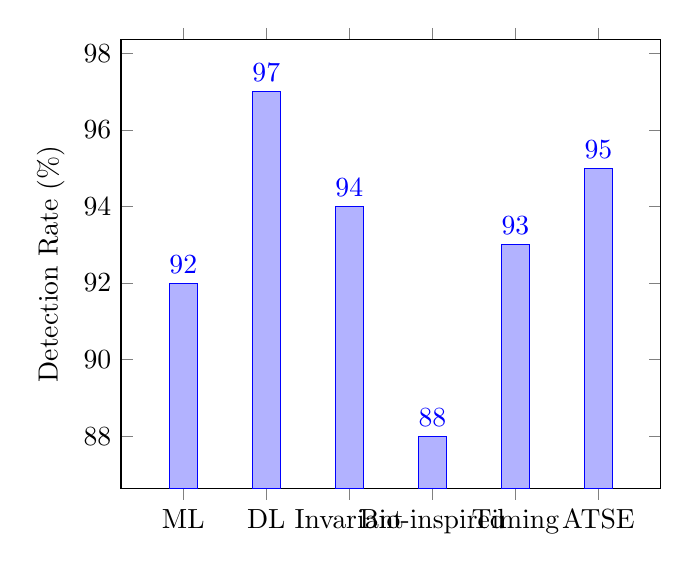
\begin{tikzpicture}
\begin{axis}[
    ybar,
    enlargelimits=0.15,
    legend style={at={(0.5,-0.15)},
      anchor=north,legend columns=-1},
    ylabel={Detection Rate (\%)},
    symbolic x coords={ML, DL, Invariant, Bio-inspired, Timing, ATSE},
    xtick=data,
    nodes near coords,
    nodes near coords align={vertical},
    ]
\addplot coordinates {(ML,92) (DL,97) (Invariant,94) (Bio-inspired,88) (Timing,93) (ATSE,95)};
\end{axis}
\end{tikzpicture}
\caption{Comparison of Detection Rates for Different Anomaly Detection Methods}
\label{fig:detection_rates}
\end{figure}

\begin{table}[h]
\centering
\caption{Applicability of Methods to Different CPS Domains}
\label{tab:applicability}
\begin{tabular}{|l|c|c|c|c|}
\hline
\textbf{Method} & \textbf{Smart Grid} & \textbf{Industrial IoT} & \textbf{Smart Cities} & \textbf{Healthcare CPS} \\
\hline
Machine Learning & \checkmark & \checkmark & \checkmark & \checkmark \\
Deep Learning & \checkmark & \checkmark & \checkmark & \checkmark \\
Invariant-based & \checkmark & \checkmark & & \checkmark \\
Bio-inspired (iDCA) & & \checkmark & \checkmark & \\
Timing-based & & \checkmark & & \\
ATSE & \checkmark & & & \\
\hline
\end{tabular}
\end{table}



\begin{figure}[h]
\centering
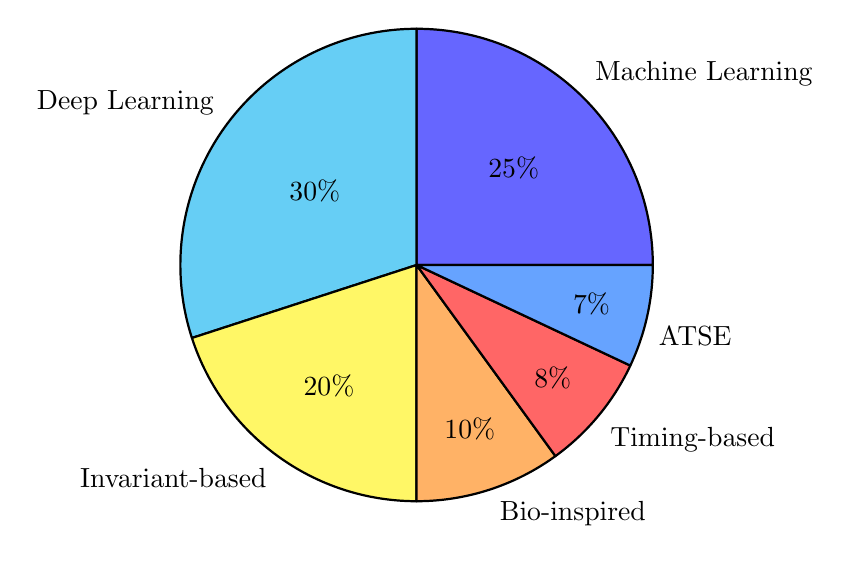
\begin{tikzpicture}
\pie{25/Machine Learning, 30/Deep Learning, 20/Invariant-based, 10/Bio-inspired, 8/Timing-based, 7/ATSE}
\end{tikzpicture}
\caption{Distribution of Research Focus in Anomaly Detection Methods}
\label{fig:research_focus}
\end{figure}

\end{comment}

\begin{comment}
\begin{table*}[h]
\centering
\caption{Comprehensive Comparison of Anomaly Detection Approaches in CPS and IoT}
\label{tab:anomaly_comparison}
\resizebox{\textwidth}{!}{%
\begin{tabular}{|l|c|c|c|c|c|c|}
\hline
\textbf{Approach} & \textbf{Scalability} & \textbf{Interpretability} & \textbf{Adaptability} & \textbf{Data Requirements} & \textbf{Computational Cost} & \textbf{Key Strengths} \\
\hline
Machine Learning & High & Medium & Medium & Medium & Medium & 
\begin{tabular}[c]{@{}c@{}}Effective for structured data; \\ Good for known patterns\end{tabular} \\
\hline
Deep Learning & Medium & Low & High & High & High & 
\begin{tabular}[c]{@{}c@{}}Excellent for complex patterns; \\ Handles high-dimensional data\end{tabular} \\
\hline
Machine Learning and Deep Learning & High & Medium & High & High & Medium-High & 
\begin{tabular}[c]{@{}c@{}}Combines strengths of ML and DL \\ for better performance\end{tabular} \\
\hline
Hybrid & High & Medium & High & Medium & Medium-High & 
\begin{tabular}[c]{@{}c@{}}Versatile and robust; \\ Combines strengths of multiple approaches\end{tabular} \\
\hline
Mathematics & High & High & Low & Medium & Low & 
\begin{tabular}[c]{@{}c@{}}Strong theoretical foundation; \\ Effective for mathematical analysis\end{tabular} \\
\hline
Invariant-based & Medium & High & Low & Low & Low & 
\begin{tabular}[c]{@{}c@{}}Strong theoretical foundation; \\ Effective for systems with clear constraints\end{tabular} \\
\hline
Other & Medium & Medium & Medium & Medium & Medium & 
\begin{tabular}[c]{@{}c@{}}Novel and adaptable; \\ Addresses niche problems effectively\end{tabular} \\
\hline
\end{tabular}%
}
\end{table*}
\end{comment}













\begin{comment}
    

\begin{table*}[h]
\centering
\caption{Comprehensive Comparison of Anomaly Detection Approaches in CPS and IoT}
\label{tab:anomaly_comparison}
\resizebox{\textwidth}{!}{%
\begin{tabularx}{\textwidth}{@{}p{3cm}XXXXXp{4cm}@{}}
\toprule
\textbf{Approach} & \textbf{Scalability} & \textbf{Interpretability} & \textbf{Adaptability} & \textbf{Data Requirements} & \textbf{Computational Cost} & \textbf{Key Strengths} \\
\midrule
Machine Learning & High & Medium & Medium & Medium & Medium & Effective for structured data; good for known patterns. \\
Deep Learning & Medium & Low & High & High & High & Excellent for complex patterns; handles high-dimensional data. \\
Machine Learning and Deep Learning & High & Medium & High & High & Medium-High & Combines strengths of ML and DL for better performance. \\
Hybrid & High & Medium & High & Medium & Medium-High & Versatile and robust; combines strengths of multiple approaches. \\
Mathematics & High & High & Low & Medium & Low & Strong theoretical foundation; effective for mathematical analysis. \\
Invariant-based & Medium & High & Low & Low & Low & Strong theoretical foundation; effective for systems with clear constraints. \\
\bottomrule
\end{tabularx}%
}
\end{table*}
\end{comment}

Table \ref{tab:anomaly_comparison} comprehensive comparison highlights the strengths and weaknesses of various anomaly detection approaches in CPS and IoT, helping identify the most suitable techniques based on specific application requirements.










\begin{comment}
    

\begin{table}[h]
\centering
\caption{Comprehensive Comparison of Anomaly Detection Approaches in CPS and IoT}
\label{tab:anomaly_comparison}
\resizebox{\textwidth}{!}{%
\begin{tabular}{|l|c|c|c|c|c|c|}
\hline
\textbf{Approach} & \textbf{Scalability} & \textbf{Interpretability} & \textbf{Adaptability} & \textbf{Data Requirements} & \textbf{Computational Cost} & \textbf{Key Strengths} \\
\hline
Machine Learning & High & Medium & Medium & Medium & Medium & 
\begin{tabular}[c]{@{}c@{}}Effective for structured data\\ Good for known patterns\end{tabular} \\
\hline
Deep Learning & Medium & Low & High & High & High & 
\begin{tabular}[c]{@{}c@{}}Excellent for complex patterns\\ Handles high-dimensional data\end{tabular} \\
\hline
Hybrid & High & Medium & High & Medium & Medium-High & 
\begin{tabular}[c]{@{}c@{}}Versatile and robust\\ Combines strengths of multiple approaches\end{tabular} \\
\hline
Invariant-based & Medium & High & Low & Low & Low & 
\begin{tabular}[c]{@{}c@{}}Strong theoretical foundation\\ Effective for systems with clear constraints\end{tabular} \\
\hline
Bio-inspired & High & Low & High & Medium & Medium & 
\begin{tabular}[c]{@{}c@{}}Highly adaptable\\ Inspired by robust natural systems\end{tabular} \\
\hline
Statistical & High & High & Low & Medium & Low & 
\begin{tabular}[c]{@{}c@{}}Well-established techniques\\ Effective for time-series data\end{tabular} \\
\hline
Graph-based & Medium & Medium & Medium & Medium & Medium & 
\begin{tabular}[c]{@{}c@{}}Captures complex relationships\\ Suitable for network-based systems\end{tabular} \\
\hline
\end{tabular}%
}
\end{table}
\end{comment}





\begin{comment}

\begin{figure}[h]
    \centering
    \includegraphics[width=0.5\textwidth]{images/output (1).png}
    \caption{Caption for the image}
    \label{fig:example-image2}
\end{figure}
\end{comment}


\subsection{Understanding the System to Detect Anomalies}
To detect anomalies in a Cyber-Physical System (CPS), it is essential to first understand the system itself. This means knowing how the system works, what normal behavior looks like, and how its components interact. An anomaly is anything that deviates from the normal behavior of the system. To identify such deviations, it is important to establish what "normal" means for the system.

Start by creating a model that shows how the different parts of the system work together. Collect data from sensors, logs, and other system components to get a clear picture of normal operations \cite{210}. Use this data to define typical patterns and acceptable ranges for important parameters like temperature, speed, or pressure. By knowing these normal ranges, it becomes easier to spot unusual behaviors. It is also helpful to consider external factors, like weather or user interactions, that might affect how the system behaves. These factors should be included in your understanding of the system to avoid false alarms. By studying how the system responds to different situations, you can learn to identify patterns that indicate problems.

In addition, understanding the system involves knowing its weaknesses. Older equipment or outdated software may introduce vulnerabilities that need extra attention. Knowing these weak points helps in designing better anomaly detection methods. Overall, understanding the system deeply is the first step to identifying problems effectively.



\subsection{Applying Approaches for Anomaly Detection}
After understanding the system and identifying anomalies, the next step is to choose the right methods to detect them. Different systems require different approaches, and it is important to select the one that best fits the needs of your CPS.

If your system's behavior is simple and predictable, statistical methods like tracking averages or thresholds might work well. For more complex systems, machine learning methods can analyze large amounts of data to detect unusual patterns. Deep learning models, such as neural networks, are especially useful for handling complicated data like images or time-series data. Once you choose a method, you need to test it to make sure it works well. Use historical data to train the model and check how accurately it detects anomalies. If the system changes over time, update the model regularly so it can keep detecting new problems effectively.
Real-time detection is also important for many CPS applications, like power grids or autonomous vehicles. Methods like edge computing can process data quickly and help detect anomalies without delays. To ensure the detection system works efficiently, set clear thresholds for when to flag a problem. These thresholds should balance being sensitive enough to catch issues while avoiding too many false alarms.

Finally, connect your anomaly detection system to actions that can fix problems. For example, if an anomaly is detected, the system might shut down a faulty machine or alert a technician. Regularly evaluate how well the system performs and improve it based on feedback. By using the right methods and continuously refining them, you can keep your CPS secure and reliable.


    
\section{Evaluating and Validating Anomaly Detection Approaches}

Evaluating and validating anomaly detection approaches is important to ensure their effectiveness and reliability. A well-validated method provides confidence that it will work as expected in real-world situations. The evaluation process can be categorized as follows:

\begin{itemize}
    \item \textbf{Using Appropriate Datasets}: Publicly available benchmark datasets are commonly used to test and compare different methods. These datasets often include labeled examples of both normal and anomalous behavior. In some cases, domain-specific data may need to be collected to reflect the unique characteristics of the system being monitored.
    \begin{itemize}
        \item \textbf{SWaT (Secure Water Treatment) Dataset}\cite{103}: Used for water treatment anomaly detection scenarios, including seven days of normal operation and four days of attack scenarios.
        \item \textbf{WADI (Water Distribution) Dataset}\cite{104}: An extension of SWaT, focusing on water distribution testbeds for cyber and physical attack simulations.
        \item \textbf{NSL-KDD Dataset}\cite{105}: A network intrusion detection dataset with categories like DoS and R2L, widely employed for training and testing models.
        \item \textbf{Bot-IoT Dataset}\cite{106}: Focused on IoT anomalies such as DDoS, DoS, and reconnaissance attacks, often used for IIoT-focused evaluations.
        \item \textbf{HAI Dataset}\cite{107}: Designed for simulating power systems under attack, including thermal and hydropower scenarios.
        \item \textbf{Tennessee Eastman Process (TEP) Model}\cite{108}: Simulated chemical process plant data used for evaluating detection frameworks.
        \item \textbf{BATADAL Dataset}\cite{109}: An extension of WADI for competition in attack detection, including data from 26 sensors and 17 actuators.
        \item \textbf{Edge-IIoTset2023 Dataset}\cite{70}: Features IoT/IIoT security scenarios, including Modbus flows and 14 types of attacks such as SQL Injection and Mirai UDP.
        \item \textbf{CICIoT2023 Dataset}\cite{110}: Focused on cyber portions of IoT systems, featuring 33 types of attacks.
        \item \textbf{Automotive Dataset}\cite{111}: Contains 25 hours of driving data collected from a modern car, showcasing multi-domain adaptability.
        \item \textbf{Synthetic and Simulated Datasets}\cite{112}: Generated via Hidden Markov Models (HMM) for systematic anomaly injection testing.
        \item \textbf{UNSW-NB15 Dataset}\cite{113}: An intrusion dataset for testing cybersecurity measures in IoT environments.
        \item \textbf{ICS (Industrial Control System) Dataset}\cite{7}: Focused on control systems' cyberattack scenarios, such as electric transmission disruptions.
        \item \textbf{IDA, MFP, ACS}\cite{90}: Specialized datasets for failure prediction in industrial systems, aviation, and heavy machinery.
        \item \textbf{Gas Pipeline Dataset}\cite{114}: Simulation data from a pipeline monitoring system.
        \item \textbf{CPS Custom or Experimental Datasets}\cite{115,86}: Examples include real-world CPS setups with customized data for specific attack scenarios.
    \end{itemize}
    \item \textbf{Evaluation Metrics}: Metrics like accuracy, precision, recall, and F1 score are essential for measuring the success of a methodology. Accuracy indicates overall performance, while precision focuses on the proportion of true anomalies among all detected anomalies. Recall reflects the ability to identify all actual anomalies, and the F1 score provides a balanced measure. Additionally, AUC-ROC helps evaluate the trade-off between true positive and false positive rates.
    \item \textbf{Real-World Testing}: Deploying the methodology in live or simulated environments helps assess practical performance. This includes examining how well it handles real-time data streams, adapts to changes in the system, and minimizes false positives and negatives.
    \item \textbf{Robustness Testing}: Methods should be tested under challenging conditions, such as noisy data, missing values, or adversarial scenarios. This ensures the approach remains reliable even in less-than-ideal conditions.
    \item \textbf{Scalability Assessment}: The method's performance should be analyzed as data size and complexity increase. Computational efficiency is also a critical factor, particularly in systems with resource constraints.
    \item \textbf{Feedback and Iterative Improvement}: Input from domain experts and operators can provide valuable insights for refinement. The detection model should be continuously updated with new data and evolving conditions to improve accuracy and reliability.
    \item \textbf{Comparative Analysis}: Comparing the performance of the methodology against other state-of-the-art approaches helps identify its strengths and weaknesses in terms of accuracy, speed, and scalability. This analysis highlights areas where the method excels or needs improvement.
\end{itemize}

Through these steps, anomaly detection methodologies can be thoroughly evaluated and validated, ensuring they are both theoretically sound and practically effective for real-world applications.


\section{Real-Time Anomaly Detection}\label{sec:realtime}

Real-time anomaly detection plays a crucial role in ensuring the smooth operation of CPS. These systems, which are deeply embedded in industries such as manufacturing, transportation, and energy, integrate physical processes with digital control \cite{194,195,196,197}. They rely on sensors, networks, and software to make real-time decisions. However, when something goes wrong like a sensor failure, a cyber attack, or a system glitch it is essential to catch the problem quickly to avoid damage. That is where real-time anomaly detection steps in \cite{198,199,200}.

\subsection{Need for Real-Time Detection}

Imagine a factory running 24/7, producing goods non-stop. In such a high-paced environment, every minute counts. If one machine starts to malfunction or an attacker tries to disrupt the system, it needs to be identified instantly, before it impacts the entire production line. A delay in detection could cause equipment breakdowns, safety hazards, or even financial losses. This is especially true in autonomous vehicles or power grids, where a small delay in detecting a malfunction could mean life-threatening accidents or power outages \cite{98,99}.

So, the challenge is clear: detect problems as soon as they occur, with minimal delay. But doing this in real-time is not easy. CPS are complex systems, often generating huge amounts of data from various sensors. Processing this data quickly and accurately requires advanced technology \cite{101,60}.

\subsection{Challenges of Real-Time Detection}

One of the biggest challenges in real-time anomaly detection is latency the system needs to react fast, without causing delays in operations. For instance, a smart grid must continue to provide electricity while monitoring for any anomalies, like unusual power consumption patterns. If the system takes too long to detect the anomaly, it could lead to power failures \cite{50}.

Another challenge is dealing with noisy data. Sensors in CPS can generate a lot of unnecessary or incorrect data, which can confuse the detection system. Imagine a factory where one sensor is faulty and constantly gives wrong readings. If the detection system can not filter out this noise, it might either miss the real problem or give too many false alarms \cite{98,60}.

Additionally, CPS environments often produce imbalanced data, meaning that the system operates normally most of the time, with only a few instances of anomalies. This makes it harder for detection systems to learn from past problems and detect new ones \cite{60,50}.

\subsection{Approaches to Real-Time Anomaly Detection}

To tackle these challenges, researchers have developed several approaches to real-time anomaly detection. These methods range from traditional statistical techniques to cutting-edge machine learning and deep learning models.

\subsubsection{Hybrid Models}
A common solution is to use hybrid models that combine both traditional statistical methods and machine learning. For example, models like \textit{SARIMA} (Seasonal Autoregressive Integrated Moving Average) can predict future sensor readings based on past data. When combined with machine learning models like LSTM (Long Short-Term Memory), which is great for handling time series data, these models can detect anomalies that occur over time \cite{60}. This approach is especially useful in ICS, where monitoring the normal operations of machines over time helps detect subtle changes that might indicate a problem.

\subsubsection{Deep Learning Models}
Deep learning is another powerful tool. Deep learning models, like Convolutional Neural Networks (CNNs) and Recurrent Neural Networks (RNNs), can analyze sensor data in real-time to find patterns that indicate an anomaly. For example, in autonomous vehicles, CNNs have been used to monitor sensor data from various systems, like cameras and radar, to detect any abnormal behavior \cite{97,99}. These models are particularly effective because they can automatically learn from large amounts of data, even when the patterns are complex or hidden from the human eye.

Additionally, autoencoders a type of neural network are becoming popular for real-time anomaly detection in CPS. These models are trained to recreate normal data patterns, and when they encounter something that does not fit the normal pattern, they flag it as an anomaly \cite{15}.

\subsubsection{Human-Cyber-Physical Systems (HCPS)}
With the rise of Industry 5.0, there is a growing recognition that humans should play a central role in these systems. The concept of HCPS brings humans back into the loop by integrating human expertise with the digital system's capabilities. In industries like manufacturing, human workers often have valuable experience that can help in identifying anomalies that machines might miss. For example, in a smart factory, human experts might oversee an anomaly detection system that uses big data analytics and edge computing to monitor real-time production \cite{101}.

In one case study, an HCPS system was deployed to monitor vinyl flooring production. The system combined human knowledge with machine learning to detect quality issues in real-time, sending feedback to adjust machine operations automatically \cite{101}. This approach highlights how human input can enhance the detection system, especially in environments where machine-learning models might struggle with the complexity or variability of the data.

\subsubsection{Edge Computing for Low Latency}
Edge computing is a technology that processes data close to where it is generated, rather than sending it all to a central server. This reduces the time it takes to analyze the data and send back a decision. In a smart factory, edge computing might be used to monitor machines and detect problems as they happen, without the delays that come with cloud computing \cite{100,101}. This is particularly useful in real-time anomaly detection, as decisions need to be made instantly.

\subsubsection{Adversarial Machine Learning and Evasion Attacks}
As CPS systems become smarter, so do the attackers. Adversarial machine learning involves using techniques to fool detection systems into missing an anomaly or incorrectly classifying normal data as a problem. For example, attackers might manipulate sensor readings to look normal, while in reality, they are carrying out an attack. This is known as an evasion attack \cite{96}. To counter this, researchers have developed machine learning models that are trained to recognize these subtle, adversarial changes in the data, making real-time detection systems more resilient to sophisticated attacks \cite{96}.

\subsection{Real-World Applications of Real-Time Anomaly Detection}

Real-time anomaly detection is being applied in various fields:

\begin{itemize}
    \item \textbf{Industrial Manufacturing:} Factories use real-time monitoring systems to ensure that machines operate smoothly. If a machine starts behaving abnormally, the system can immediately alert operators or shut down the machine to prevent further damage \cite{100}.
    \item \textbf{Autonomous Vehicles:} In self-driving cars, real-time anomaly detection ensures that all sensors and systems are working correctly. If a sensor starts malfunctioning, the car can respond by switching to backup systems or pulling over safely \cite{97,98}.
    \item \textbf{Smart Grids:} Power grids use real-time detection to monitor electricity usage and detect any unusual patterns, which could indicate a cyber-attack or system failure \cite{98}.
\end{itemize}

\subsection{Future Directions}

Looking to the future, the focus will be on improving the scalability and resilience of real-time anomaly detection systems. One promising direction is the use of \textit{decentralized detection}, where anomalies are detected locally at different points in the system, rather than relying on a central system. This approach is expected to make systems more robust and less vulnerable to single points of failure \cite{50}.

Another exciting development is the integration of blockchain technology, which could enhance the security and integrity of the data used for anomaly detection. By ensuring that data cannot be tampered with, blockchain could make real-time anomaly detection even more reliable in sensitive environments like power grids and healthcare \cite{101}.

\section{Future Work}\label{sec:future}

The field of anomaly detection in Cyber-Physical Systems (CPS) continues to grow, but there are still many challenges and opportunities for improvement. Machine learning and deep learning methods have significantly improved anomaly detection, but they remain vulnerable to attacks designed to trick them. Future research should focus on creating more robust systems. Techniques like training models with simulated attacks and sharing models securely without sharing data could make these systems more reliable \cite{67}. CPS environments, especially in industries like manufacturing and energy, require detection systems that can process large amounts of data quickly and work in real-time. Future work should aim to develop methods that achieve this, using technologies such as edge computing to reduce delays. Additionally, optimizing these systems for devices with limited resources, such as industrial IoT sensors, is critical to ensure practical applications.

Anomalies in CPS are rare, making it difficult to gather enough labeled data to train models effectively. Researchers should explore methods that can handle limited or imbalanced data, such as learning from small datasets, generating synthetic data, or using unsupervised approaches. These techniques could make anomaly detection more accessible and applicable to real-world systems \cite{58}. Another important area is making anomaly detection results easier to understand. Clear explanations for why an anomaly is detected will help users trust and act on the system's findings. Future research should focus on creating interpretable models that provide actionable insights, which are essential in critical infrastructure applications.

Domain-specific knowledge can greatly enhance anomaly detection systems. Combining data-driven models with physical simulations or rules, like those used in digital twins, could improve their accuracy and relevance.Expanding anomaly detection methods to other fields, such as healthcare, autonomous vehicles, and energy systems, offers exciting opportunities. Developing flexible and adaptable models will ensure that these methods can perform effectively in diverse applications. Future research should also aim to establish standard datasets, testing methods, and performance measures to allow consistent evaluation and comparison of these techniques.

As CPS systems increasingly handle sensitive data, ensuring privacy and addressing ethical concerns is crucial. Researchers should prioritize creating methods that protect data while detecting anomalies, using tools like differential privacy and secure multi-party computation. Addressing these issues will make these systems safer and more trustworthy. By focusing on these areas, future research can make anomaly detection systems more robust, scalable, and practical, ultimately helping to build safer and more reliable CPS environments.

\section{Conclusion}\label{sec:conclusion}
Anomaly detection in Cyber-Physical Systems (CPS) is a crucial research area with widespread applications in critical sectors like energy, transportation, and healthcare. This review has summarized key findings from existing literature, covering a range of approaches including machine learning, deep learning, hybrid models, and domain-specific techniques. Each method offers unique strengths but also has limitations, such as difficulty in handling rare events, challenges in achieving real-time processing, and vulnerabilities to adversarial attacks.

Table \ref{tab:anomaly_comparison} provides a comparison of different approaches for problem-solving in anomaly detection, highlighting their capabilities, strengths, limitations, and examples. These approaches range from mathematical models and machine learning to hybrid and invariant-based methods, showcasing the diverse strategies available to tackle the challenges in CPS. While hybrid approaches demonstrate flexibility and the ability to detect a wide variety of problems, other methods such as invariant-based techniques excel in rule-based validations, emphasizing the importance of selecting the right approach based on the application context.

A significant gap identified in the literature is the lack of methods that are both scalable and interpretable while ensuring privacy and security in diverse CPS environments. Additionally, the reviewed studies emphasize the importance of integrating domain knowledge to improve detection accuracy and relevance. The implications of these findings suggest that future research should prioritize the development of robust and adaptive anomaly detection systems. These systems must address the current challenges by incorporating explainable AI, leveraging domain-specific insights, and adhering to ethical and privacy standards. Such advancements are necessary to enhance the reliability and safety of CPS, especially as they become increasingly complex and interconnected.

By building on the strengths and addressing the gaps highlighted in this review, researchers and practitioners can contribute to a more secure and resilient CPS ecosystem, ensuring its continued efficiency and trustworthiness in critical applications.





% References

\bibliographystyle{IEEEtran}
\bibliography{refs}


\end{document}